\chapter{Preliminaries}%
\label{chap:preliminaries}%
\graphicspath{{./chapters/preliminaries/scripts/}}%
In\marginnote{\footnotesize \textbf{Contents:}\\\localtableofcontents} this chapter, we recall important mathematical concepts that are used in the remainder of this thesis.
In particular, we recall standard results from functional analysis, probability theory, stochastic differential equations, and optimization and define our notion of images as signals defined on a finite Cartesian grid.
This chapter serves primarily as a reference, with no new contributions.
Subsequent chapters will refer back to the definitions, theorems, and algorithms discussed here as needed.
However, \cref{sec:pdes} on stochastic differential equations and \cref{sec:optimization} on optimization discuss some peculiarities of how the concepts are used in this thesis.
\section{Functional analysis}
In this section, we recall definitions and results from analysis, topology, and measure theory used in the subsequent sections.
This overview is adapted from~\cite{Alt2016,beck_firstorder_2017,Klenke2014}.
In this thesis, the field \( \Field \) are either the real numbers \( \R \) or the complex numbers \( \C \).
For any \( x \in \Field \), we denote the absolute value by
\begin{equation}
	\abs{x} \coloneqq \sqrt{x\conj{x}}\ \text{with}\ \conj{x} = \begin{cases}
		\mathfrak{Re}(x) - \mathfrak{Im}(x) &\ \text{if}\ \Field = \C, \\
		x &\ \text{if}\ \Field = \R.
	\end{cases}
\end{equation}
\subsection{Vector spaces}
\begin{definition}[Vector space]%
	\label{def:vector space}
	A \emph{vector space} over a field \( \Field \) is a nonempty set \( \V \) endowed with a binary function \( \map{(\argm +_{\V} \argm)}{\V \times \V}{\V} \) (\enquote{vector addition}) and a binary function \( \map{(\argm \cdot_{\V} \argm)}{\Field \times \V}{\V} \) (\enquote{scalar multiplication}) such that the following holds:
	\begin{enumerate}
		\item Let \( x \), \( y \), and \( z \) be arbitrary elements of \( \V \). The vector addition satisfies
		\begin{enumerate}
			\item \( x +_{\V} (y +_{\V} z) = (x +_{\V} y) +_{\V} z. \)
			\item \( x +_{\V} y = y +_{\V} x. \)
			\item There exists a unique element \( \num{0}_{\V} \in \V \) such that \( x +_{\V} \num{0}_{\V} = x \).
			\item There exists an element \( -x \in \V \) such that \( x +_{\V} (-x) = \num{0} \).
		\end{enumerate}
		\item Let \( a \) and \( b \) be arbitrary elements of the field \( \Field \) and let \( x \) be an arbitrary element of \( \V \). The scalar multiplication satisfies
		\begin{enumerate}
			\item \( a\cdot_{\V}(b\cdot_{\V}x) = (a\cdot_{\V}b)\cdot_{\V}x \).
			\item Let \( \num{1}_{\Field} \) denote the multiplicative identity in \( \Field \). Then \( \num{1}_{\Field}\cdot_{\V}x = x \).
		\end{enumerate}
		\item The scalar multiplication distributes with respect to vector addition and field addition:
		\begin{enumerate}
			\item \( a\cdot_{\V}(x +_{\V} y) = a\cdot_{\V}x +_{\V} a\cdot_{\V}y \).
			\item \( (a +_{\Field} b)\cdot_{\V}x = a\cdot_{\V}x +_{\V} b\cdot_{\V}x \).
		\end{enumerate}
	\end{enumerate}
\end{definition}

The most prominent example of a vector space is \( \R^n \).
Its base field are the real numbers \( \R \), the set \( \V \) are all \( n \)-tuples with real components and vector addition and scalar multiplication are defined as
\begin{equation}
	\begin{pmatrix}
		x_{\num{1}} \\ x_{\num{2}} \\ \vdots \\ x_n
		\end{pmatrix} +_{\R^n} \begin{pmatrix}
		y_{\num{1}} \\ y_{\num{2}} \\ \vdots \\ y_n
	\end{pmatrix} = \begin{pmatrix}
	x_{\num{1}} +_{\R} y_{\num{1}} \\ x_{\num{2}} +_{\R} y_{\num{2}} \\ \vdots \\ x_n +_{\R} y_n
	\end{pmatrix},\quad a\cdot_{\R^n} \begin{pmatrix}
	x_{\num{1}} \\ x_{\num{2}} \\ \vdots \\ x_n
	\end{pmatrix} = \begin{pmatrix}
	a\cdot_{\R}x_{\num{1}} \\ a\cdot_{\R}x_{\num{2}} \\ \vdots \\ a\cdot_{\R}x_n
	\end{pmatrix}.
\end{equation}
Here \( x = (x_{\num{1}}, x_{\num{2}}, \dotsc, x_n)\tp \), \( y = (y_{\num{1}}, y_{\num{2}}, \dotsc, y_n)\tp \in \R^n \) and \( a \in \R \).
In this thesis, it is not necessary to distinguish between the set of a vector space and the vector space itself (the (set, addition, multiplication) triple).
In other words, \( \R^n \) refers to the \emph{vector space} and implicitly carries over the operations as defined above.

\subsection{Inner products}
It is well known that two vectors in \( \R^n \) are \emph{orthogonal}, if their \emph{dot product} is zero.
As a generalization of the dot product, inner products can be used to impose geometry onto a vector space by mapping a pair of vectors to a scalar in the underlying field.
\begin{definition}[Inner product]%
	\label{def:inner product}
	Let \( \V \) be a vector space over a field \( \Field \).
	An \emph{inner product} \( \map{\inprod{\argm}{\argm}_{\V}}{\V \times \V}{\Field} \) satisfies
	\begin{enumerate}
		\item \( \inprod{x}{y}_{\V} = \conj{\inprod{y}{x}_{\V}} \) for any \( x , y \) in \( \V \).
		\item \( \inprod{a_{\num{1}} x_{\num{1}} + a_{\num{2}} x_{\num{2}}}{y}_{\V} = a_{\num{1}}\inprod{x_{\num{1}}}{y}_{\V} + a_{\num{2}}\inprod{x_{\num{2}}}{y}_{\V} \) for any \( a_{\num{1}}, a_{\num{2}} \in \Field \) and any \( x, y \in \V \).
		\item \( \inprod{x}{x}_{\V} \geq \num{0} \) for any \( x \in \V \) and \( \inprod{x}{x}_{\V} \) if and only if \( x = \num{0}_{\V} \).
	\end{enumerate}
\end{definition}
We call the ordered pair \( (\V, \inprod{\argm}{\argm}_{\V}) \) an \emph{inner product space}.
The aforementioned dot product on \( \R^n \) is the map
\begin{equation}
	\inprod{x}{y}_{\R^n} = \sum_{i={\num{1}}}^n x_i y_i.
\end{equation}
\subsection{Norms}
We use norms to rigorously define notions of distance from the origin in a vector space.
In particular, any sensible distance function should absolutely commute with scaling, obey the triangle inequality, and assign zero only to the zero vector.
This motivates the following definition:
\begin{definition}[Norm]%
	\label{def:norm}
	Let \( \V \) be a vector space over a field \( \Field \).
	A norm \( \map{\norm{}_{\V}}{\V}{\R} \) satisfies
	\begin{enumerate}
		\item \( \norm{ax}_{\V} = \abs{a}\,\norm{x}_{\V} \) for any \( x \in \V \) and \( a \in \Field \).\label{def:norm item one}
		\item \( \norm{x + y}_{\V} \leq \norm{x}_{\V} + \norm{y}_{\V} \) for all \( x, y \in \V \).\label{def:norm item two}
		\item \( \norm{x}_{\V} = \num{0} \implies x = \num{0}_{\V} \).
	\end{enumerate}
\end{definition}
Note that~\cref{def:norm item one} implies \( \norm{\num{0}_{\V}}_{\V} = \num{0} \) and that~\cref{def:norm item one} and~\cref{def:norm item two} imply nonnegativity: \( \norm{x}_{\V} \geq \num{0} \), another sensible property of a distance function.

A function that satisfies~\cref{def:norm item one} and~\cref{def:norm item two} but maps some nonzero vectors to zero is called a \emph{seminorm}.
The ordered pair \( (\V, \norm{}_{\V}) \) is called a \emph{normed vector space}.
Any inner product on a vector space \( \V \) induces a norm through \( \norm{}_{\V} = \sqrt{\inprod{\argm}{\argm}}_{\V} \).

In the previous definitions, we endowed the operations of vector addition, scalar multiplication, inner product, and norms with a subscript to emphasize the vector space these operations occur in.
However, this notation is overly verbose and usually the space is evident from the context.
Thus, in the remainder of this thesis we omit this subscript unless needed.

An important family of norms are the \( \ell^p \) norms on \( \Field^n \) defined as
\begin{equation}
	\norm{x}_{p} \coloneqq \begin{cases}
		\displaystyle\biggl( \sum_{i=\num{1}}^n \abs{x_i}^p\biggr)^{\frac{1}{p}} &\ \text{if}\ \num{1} \leq p < \infty, \\
		\displaystyle\max_{i=\num{1},\dotsc,n} \abs{x_i} &\ \text{if}\ p = \infty.
	\end{cases}
\end{equation}
\begin{sidefigure}
	\begin{tikzpicture}
		\begin{axis}[
			legend image with text/.style={%
				legend image code/.code={%
					\node[anchor=center] at (0cm,0cm) {#1};
				}
			},
			legend columns=-1,
			legend image code/.code={%
				\draw[mark repeat=2,mark phase=2,#1] 
					plot coordinates {
						(0cm,0cm) 
						(0.2cm,0cm)
						(0.4cm,0cm)
					};
			},
			legend style={%
				font=\fontsize{7pt}{8pt}\selectfont,
				at={(0.0, 1.05)},
				anchor=west,
				draw=none
			},
			trig format plots=rad,
			axis equal,
			width=4cm,
			scale only axis,
			marginplot,
			xmin=-1.2, xmax=1.2,
			ymin=-1.2, ymax=1.2,
			axis on top,
			thick,
		]
			\addlegendimage{legend image with text={}}
			\addlegendentry{$p=$}
			\addplot+ coordinates {(0, 1) (-1, 0) (0, -1) (1, 0) (0, 1)};
			\addlegendentry{$1$}
			\addplot+ [domain=0:2*pi, samples=200] ({sin(x)}, {cos(x)});
			\addlegendentry{$2$}
			\addplot+ [raw gnuplot] gnuplot {%
				set isosamples 500;
				set contour base;
				set cntrparam levels discrete 1.0;
				unset surface;
				set xrange [-1.1:1.1];
				set yrange [-1.1:1.1];
				splot (abs(x)**5+abs(y)**5)**(1./5.);
			};
			\addlegendentry{$5$}
			\addplot+ coordinates {(1,1) (-1,1) (-1,-1) (1,-1) (1,1)};
			\addlegendentry{$\infty$}
		\end{axis}
	\end{tikzpicture}
	\caption[Unit spheres of \( p \)-norms]{%
		Unit spheres of different \( p \)-norms in \( \R^{\num{2}} \).
	}%
	\label{fig:norm balls}
\end{sidefigure}
\Cref{fig:norm balls} visualizes the unit spheres of different \( \ell^p \) norms in \( \R^{\num{2}} \):
The unit-one-norm-sphere is a rhombus, the unit-two-norm-sphere is a circle and as \( p \) approaches infinity, the unit-\( p \)-norm-sphere approaches a square.
\subsection{Topology}
In this section, we recall topological concepts that are required for understanding the optimization algorithms used in this thesis.
To proceed, we first define norm balls:
Let \( (\V, \norm{}) \) be a normed vector space.
We denote with
\begin{equation}
	\Ball{\norm{}}{c}{r} \coloneqq \Set{x \in \V \given \norm{x - c} < r}
\end{equation}
the open norm ball with respect to the norm \( \norm{} \) and radius \( r > \num{0} \), centered around \( x \in \V \).

A set \( S \subseteq \V \) is
\begin{itemize}
	\item \emph{bounded} if there exists a radius \( r > \num{0} \) such that \( S \subset \Ball{\norm{}}{\num{0}_{\V}}{r} \).
	\item \emph{open} if for all \( x \in S \) there exists an \( \epsilon > \num{0} \) such that \( \Ball{\norm{}}{x}{\epsilon} \subset S \).
	\item \emph{closed} if \( \V \setminus S \) is open.
	\item \emph{compact} if every open cover of \( S \) has a finite subcover.
\end{itemize}
The last definition is somewhat technical and overkill for our purposes --- thus we recall the simpler definition of compactness in the Euclidean case:
\begin{theorem}[Heine-Borel Theorem]%
	\label{def:heine-borel}
	Let \( S \subset \Field^n \).
	Then, the following statements are equivalent:
	\begin{itemize}
		\item \( S \) is bounded and closed.
		\item Every open cover of \( S \) has a finite subcover.
	\end{itemize}
\end{theorem}
Other basic notions that we will need for the rest of this section are the interior and the closure of a set:
\begin{definition}[Interior, closure, boundary]%
	\label{def:interior closure boundary}
	Let \( (\V, \norm{}) \) be a normed vector space and let \( S \subseteq \V \).
	\begin{itemize}
		\item A point \( x \in S \) is an \emph{interior point} of \( S \) if there exists an open set \( O \subseteq S \) such that \( x \in O \).
			The set of all interior points forms the \emph{interior} of \( S \), denoted by \( \Interior{S} \).
		\item A point \( x \in \V \) is a \emph{point of closure} of \( S \) if for every open set \( O \subseteq S \) that contains \( x \) there exists an \( s \in S \) such that \( s \in O \).
			The set of all points of closure of \( S \) is the \emph{closure} of \( S \), denoted by \( \Closure{S} \).
		\item The \emph{boundary} of \( S \) is the set \( \Boundary{S} \coloneqq \Closure{S} \setminus \Interior{S} \).
	\end{itemize}
\end{definition}
Finally, we define the neighborhood of a point in a normed space:
\begin{definition}[Neighborhood]%
	\label{def:neighborhood}
	Let \( (\V, \norm{}) \) be a normed vector space.
	A set \( \ASet \) is a \emph{neighborhood} of a point \( x \in \V \) if there exists a radius \( r > \num{0} \) such that \( \Ball{\norm{}}{x}{r} \) is contained in \( \ASet \).
\end{definition}
\subsection{Convergence, completeness, and continuity}
In this section, we introduce the concepts of convergence of sequences, which relates to completeness of spaces and finally continuity of functions.
In this journey, we also rigorously define Hilbert spaces.
To start, let \( (\V, \norm{}) \) be a normed vector space.
We call a map from the natural numbers to \( \V \) a \emph{sequence} and use the shorthand notation \( x^n \coloneqq x(n) \) for a sequence \( x \).
\begin{definition}[Limit and convergence of a sequence]%
	\label{def:limit and convergence of a sequence}
	A point \( x_{\num{0}} \in \V \) is the \emph{limit} of a sequence \( x \) if for all \( \epsilon > \num{0} \) there exists and \( N \in \mathbb{N} \) such that for every \( n \geq N \), \( \norm{x^n - x_{\num{0}}} < \epsilon \).
	If such a point exists, we say that \( x \) \emph{converges} to \( x_{\num{0}} \) and write \( x^n \to x_{\num{0}} \) as \( n \to \infty \) or
	\[
		\lim_{n\to\infty} x^n = x_{\num{0}}.
	\]
\end{definition}
To define the completeness of a space, we require the slightly relaxed notion of a Cauchy sequence:
\begin{definition}[Cauchy sequence]%
	\label{def:cauchy sequence}
	A sequence \( x \) is \emph{Cauchy} if for every \( \epsilon > \num{0} \) there exists an \( N \in \mathbb{N} \) such that for all \( i, j > N \)
	\[
		\norm{x^i - x^j} < \epsilon.
	\]
\end{definition}
In words, a sequence is Cauchy if the distance between iterates becomes arbitrarily small for large enough arguments.
However, a Cauchy sequence is not necessarily convergent---we will show some examples later.
Finally, we can characterize complete spaces:
\begin{definition}[Completeness]%
	\label{def:completeness}
	The normed vector space \( (\V, \norm{}) \) is \emph{complete} if every Cauchy sequence converges to an element of \( \V \).
	A \emph{Hilbert space} is an inner product space which is complete with respect to the induced norm \( \norm{} = \sqrt{\inprod{x}{x}} \).
	A \emph{Banach space} is a normed space that is complete w.r.t.\ its norm.
\end{definition}
Spaces that are not complete are easy to construct.
A famous example are the rational numbers endowed with the absolute value, \( (\mathbb{Q}, \abs{\argm}) \):
The sequence of rationals \( n \mapsto \bigl( \num{1} + n^{\num{-1}} \bigr)^n \) is Cauchy but does not converge in \( (\mathbb{Q}, \abs{\argm}) \).
In \( (\R, \abs{\argm}) \), it famously converges to Euler's constant.
The next theorem relates continuity of a function with the convergence of the image a sequence under the function.
To state it, we first define continuity.
For the following, we let \( (\V, \norm{}_{\V}) \) and \( (\mathbb{W}, \norm{}_{\mathbb{W}}) \) be two normed vector spaces.
\begin{definition}[Continuity]%
	\label{def:continuity}
	A function \( \map{f}{\V}{\mathbb{W}} \) is \emph{continuous at \( x_{\num{0}} \in \V \)} if for all \( \epsilon > \num{0} \) there exists a \( \delta > \num{0} \) such that \( \norm{x - x_{\num{0}}}_{\V} < \delta \) implies that \( \norm{f(x) - f(x_{\num{0}})}_{\mathbb{W}} < \epsilon \).
\end{definition}
Let \( S \subseteq V \).
We call \( f \) \emph{continuous on \( S \)} if it is continuous at every point in \( S \).
We call \( f \) \emph{continuous} if it continuous on \( \V \).
\begin{theorem}
	Let \( \map{f}{\V}{\mathbb{W}} \).
	The following statements are equivalent:
	\begin{itemize}
		\item \( f \) is continuous.
		\item For every set \( S \subseteq \mathbb{W} \) open in \( \mathbb{W} \), the preimage of \( S \) under \( f \) is open in \( \V \).
		\item For every \( x_{\num{0}} \in \V \) and every sequence \( x \) on \( \V \) such that \( x^n \to x_{\num{0}} \) in \( \V \) the sequence \( f(x^n) \to f(x_{\num{0}}) \) in \( \mathbb{W} \) as \( n \to \infty \).
	\end{itemize}
\end{theorem}
\begin{proof}
	See~\cite[section 2.17]{Alt2016}.
\end{proof}

The optimization algorithms we use in this thesis often have slightly stronger assumptions on functions.
In particular, they often require that the distance of the images of two points can be upper bounded by their distance, up to a multiplicative constant.
This is captured in the notion of Lipschitz continuity:
\begin{definition}[Lipschitz continuity]%
	\label{def:lipschitz continuity}
	A function \( \map{f}{\V}{\mathbb{W}} \) is called \emph{Lipschitz continuous} with \emph{Lipschitz constant} \( L > \num{0} \) if for all \( x, y \in \V \)
	\[
		\norm{f(x) - f(y)}_{\mathbb{W}} \leq L \norm{x - y}_{\V}.
	\]
\end{definition}
Lipschitz continuity is illustrated for a map from \( \R \) to \( \R \) in~\cref{fig:lipschitz continuity}.
\begin{sidefigure}
	\centering
	\begin{tikzpicture}% TODO: fix this with clip false... I don't like it
		\begin{axis}[marginplot, width=.95\marginparwidth,ymin=-1, ymax=1]
			\addplot [thick, maincolor, domain=-3:3] {0.9*tanh(x - 1)};
			\addplot [domain=0:2] {x - 1};
			\addplot [domain=0:2] {-x + 1};
			\fill [opacity=.2, maincolor] (1, 0) -- (0, 1) -- (-3, 1.2) -- (-3, -1.2) -- (0, -1) -- cycle;
			\fill [opacity=.2, maincolor] (1, 0) -- (2, 1) -- (3, 1.20666) -- (3, -1.20666) -- (2, -1) -- cycle;
		\end{axis}
	\end{tikzpicture}
	\caption[Geometric interpretation of Lipschitz continuity]{Geometric interpretation of Lipschitz continuity for a function over \( \R \).}%
	\label{fig:lipschitz continuity}
\end{sidefigure}
There, the dark green function always stays outside of the double cone spanned by the two black lines.
Classical examples of functions which are not Lipschitz continuous are the exponential function and the quadratic \( x \mapsto x^{\num{2}} \) over \( \R \), and \( \sqrt{\argm} \) over \( \R_+ \).
The former two examples become infinitely steep as their arguments explode, the latter becomes infinitely steep as its argument approaches zero as illustrated in~\cref{fig:sqrt not lipschitz}.
\begin{sidefigure}
	\begin{tikzpicture}[spy using outlines={rectangle, magnification=2, size=2cm, connect spies}]
		\begin{axis}[marginplot, width=.85\marginparwidth,yticklabels={}]
			\addplot [thick, maincolor, domain=0:1, samples=201] {sqrt(x)};
			\addplot [domain=0:.2] {5*x};
			\coordinate (on) at (0.07, 0.11);
			\coordinate (at) at (0.66, 0.3);
		\end{axis}
		\spy [black, overlay] on (on) in node at (at);
	\end{tikzpicture}
	\caption[\( \sqrt{\argm} \) over \( \interval{\num{0}}{\num{1}} \) is not Lipschitz continuous]{%
		\( \sqrt{\argm} \) over \( \interval{\num{0}}{\num{1}} \) is not Lipschitz continuous.
	}%
	\label{fig:sqrt not lipschitz}
\end{sidefigure}
These examples demonstrate that Lipschitz continuity is rather strong;
often it suffices that a function satisfies Lipschitz continuity \emph{locally}:
\begin{definition}[Local Lipschitz continuity]%
	\label{def:local lipschitz continuity}
	A function \( \map{f}{\V}{\mathbb{W}} \) is \emph{locally Lipschitz continuous} if for all \( x \in \V \) there exists a neighborhood (\cref{def:neighborhood}) \( N(x) \) such that the restriction of \( f \) to \( N(x) \) is Lipschitz continuous.
\end{definition}
\subsection{Measure theory}
In this section we briefly introduce concepts from measure theory.
It is mostly based on~\cite{bredies_mathematical_2018} and is by no means a complete overview of the field---its purpose is to introduce Lebesgue spaces and lay the foundations for probability theory.

Throughout the following discussion, we denote with \( \ASet \) an arbitrary non-empty set.
We denote with \( \PowerSet{\ASet} \coloneqq \Set*{\mathcal{A} \given \mathcal{A} \subseteq \ASet} \) the power set of \( \ASet \).
First, we classify sets according to closedness properties.
\begin{definition}[Closedness properties]
	Let \( \SigmaAlgebraSymbol \subseteq \PowerSet{\ASet}\) be a set of subsets, let \( \mathcal{A}, \mathcal{A}_i, \mathcal{B} \), \( i \in \mathbb{N} \) be arbitrary elements of \( \SigmaAlgebraSymbol \), and let \( \mathcal{I} \subseteq \mathbb{N} \) be a finite or infinite subset of the natural numbers.
	The set of sets \( \SigmaAlgebraSymbol \) is
	\begin{itemize}
		\item \emph{closed under intersections} if \( \mathcal{A} \cap \mathcal{B} \in \SigmaAlgebraSymbol \).
		\item \emph{closed under countable intersections} if \( \bigcap_{i \in \mathcal{I}}\mathcal{A}_i \in \SigmaAlgebraSymbol \).
		\item \emph{closed under unions} if \( \mathcal{A} \cup \mathcal{B} \in \SigmaAlgebraSymbol \).
		\item \emph{closed under countable unions} if \( \bigcup_{i \in \mathcal{I}}\mathcal{A}_i \in \SigmaAlgebraSymbol \).
		\item \emph{closed under differences} if \( \mathcal{A} \setminus \mathcal{B} \in \SigmaAlgebraSymbol \).
		\item \emph{closed under complements} if \( \mathcal{S} \setminus \mathcal{A} \in \SigmaAlgebraSymbol \).
	\end{itemize}
\end{definition}

The subsequent discussion of probability theory heavily relies on \SigmaAlgebras, which we now define and \emph{measurable spaces}, which we now define.
\begin{definition}[\SigmaAlgebra]%
	\label{def:sigma algebra}
	A set of subsets \( \SigmaAlgebraSymbol \subseteq \PowerSet{\ASet} \) is a \emph{\SigmaAlgebra{} on \( \ASet \)} if
	\begin{itemize}
		\item \( \ASet \in \SigmaAlgebraSymbol \).
		\item \( \SigmaAlgebraSymbol \) is closed under complements.
		\item \( \SigmaAlgebraSymbol \) is closed under countable unions.
	\end{itemize}
\end{definition}
\begin{definition}[Measurable space and measurable sets]%
	\label{def:measurable spaces and measureable sets}
	A pair \( (\ASet, \SigmaAlgebraSymbol) \), where \( \ASet \) is an arbitrary nonempty set and \( \SigmaAlgebraSymbol \) is a \SigmaAlgebra{} over \( \ASet \), is a \emph{measurable space}.
	The sets in \( \SigmaAlgebraSymbol \) are called \emph{measurable}.
\end{definition}
The smallest \SigmaAlgebra{} that contains a set of subsets \( \mathfrak{E} \) is called the \SigmaAlgebra{} \emph{induced} (or \emph{generated}) by \( \mathfrak{E} \), and we write \( \sigma(\mathfrak{E}) \).
For a normed vector space \( (\V, \norm{}) \) the \SigmaAlgebra{} generated by all open sets is the \emph{Borel \SigmaAlgebra} \( \BorelSigma{\ASet} \) on \( \ASet \) and its elements are \emph{Borel measurable}.

Later, we will need the notion of \SigmaAlgebras{} that are generated by (possibly more than) one map.
\begin{definition}[Generated \SigmaAlgebra~{\cite[Definition 1.79]{Klenke2014}}]%
	\label{def:generated sigma algebra}
	Let \( \ASet \) be a nonempty set and let \( I \) be an arbitrary index set.
	For any \( i \in I \) let \( (\ASet_i, \SigmaAlgebraSymbol_i) \) be a measurable space and let \( \map{X_i}{\ASet}{\ASet_i} \) be an arbitrary map.
	Then
	\begin{equation}
		\sigma(X_i, i \in I) \coloneqq \sigma\biggl( \bigcup_{i \in I} \sigma(X_i) \biggr) \coloneqq \sigma\biggl( \bigcup_{i\in I} \PreImage{X_i}(\ASet_i) \biggr)
	\end{equation}
	is the \SigmaAlgebra{} on \( \ASet \) that is \emph{generated} by \( (X_i, i \in I) \).
	This is the smallest \SigmaAlgebra{} with respect to which all \( X_i \) are measurable.
\end{definition}

Now we develop \emph{measures} to meaningfully quantify the \enquote{size} of sets.
First, we recall properties of functions on sets and then define the notion of a \emph{measure}.
\begin{definition}[Properties of functions on sets]%
	\label{def:properties of functions on sets}
	Let \( \SigmaAlgebraSymbol \subseteq \PowerSet{\ASet} \) and let \( \map{\Measure}{\SigmaAlgebraSymbol}{\interval{\num{0}}{\infty}} \) be a function on sets.
	\( \Measure \) is
	\begin{itemize}
		\item \emph{monotone} if \( \Measure(\mathcal{A}) \leq \Measure(\mathcal{B}) \) for any \( \mathcal{A}, \mathcal{B} \in \SigmaAlgebraSymbol \) such that \( \mathcal{A} \subseteq \mathcal{B} \).
		\item \emph{additive} if \( \Measure\bigl(\bigcup_{i=\num{1}}^n \mathcal{A}_i \bigr) = \sum_{i=1}^n \Measure(\mathcal{A}_i) \) for any mutually disjoint \( \mathcal{A}_{\num{1}},\mathcal{A}_{\num{2}},\allowbreak\dotsc,\allowbreak\mathcal{A}_n \in \SigmaAlgebraSymbol \) such that \( \bigcup_{i=\num{1}}^n \mathcal{A}_i \in \SigmaAlgebraSymbol \).
		\item \emph{\(\sigma\)-additive} if \( \Measure\bigl(\bigcup_{i\in\mathbb{N}} \mathcal{A}_i \bigr) = \sum_{i\in\mathbb{N}} \Measure(\mathcal{A}_i) \) for any mutually disjoint \( \mathcal{A}_{\num{1}},\allowbreak\mathcal{A}_{\num{2}},\allowbreak\dotsc \in \SigmaAlgebraSymbol \) such that \( \bigcup_{i\in \mathbb{N}} \mathcal{A}_i \in \SigmaAlgebraSymbol \).
		\item \emph{subadditive} if \( \Measure\bigl(\bigcup_{i=1}^n \mathcal{A}_i \bigr) \leq \sum_{i=\num{1}}^n \Measure(\mathcal{A}_i) \) for any \( \mathcal{A}_{1},\mathcal{A}_{\num{2}},\dotsc,\mathcal{A}_n \in \SigmaAlgebraSymbol \) such that \( \bigcup_{i=1}^n \mathcal{A}_i \in \SigmaAlgebraSymbol \).
		\item \emph{\(\sigma\)-subadditive} if \( \Measure\bigl(\bigcup_{i=1}^n \mathcal{A}_i \bigr) \leq \sum_{i\in\mathbb{N}} \Measure(\mathcal{A}_i) \) for any \( \mathcal{A}_{1},\mathcal{A}_{\num{2}},\dotsc \in \SigmaAlgebraSymbol \) such that \( \bigcup_{i\in\mathbb{N}} \mathcal{A}_i \in \SigmaAlgebraSymbol \).
	\end{itemize}
\end{definition}
\begin{definition}[Measure]%
	\label{def:measure}
	Let \( (\ASet, \SigmaAlgebraSymbol) \) be a measurable space.
	A function \( \map{\Measure}{\SigmaAlgebraSymbol}{\interval{\num{0}}{\infty}} \) is a \emph{measure} on \( (\ASet, \SigmaAlgebraSymbol) \) if
	\begin{itemize}
		\item \( \Measure(\emptyset) = \num{0} \) and
		\item \( \Measure \) is subadditive.
	\end{itemize}
\end{definition}
The following enumerates \enquote{intuitive} measures that also find applications in this thesis:
\begin{enumerate}
	\item \emph{Counting measure:}
		Let \( (\ASet, \PowerSet{\ASet}) \) with \( \ASet \) nonempty be a measurable space.
		The \emph{counting measure} on \( (\ASet, \PowerSet{\ASet}) \)
		\begin{equation}
			\Measure(\mathcal{A}) = \begin{cases}
				\text{the number of elements in}\ \mathcal{A} &\ \text{if}\ \mathcal{A}\ \text{is finite}, \\
				\infty & \text{else,}
			\end{cases}
		\end{equation}
		assigns to any set the number of contained elements.
	\item \emph{Dirac measure:}
		Let \( \ASet \subseteq \R^n \) be nonempty and \( (\ASet, \BorelSigma{\ASet}) \) be a measurable space.
		The \emph{Dirac measure} on \( (\ASet, \BorelSigma{\ASet}) \)
		\begin{equation}
			\Dirac_{x}(\mathcal{A}) = \begin{cases}
				\num{1} & \text{if } x \in \mathcal{A},\\
				\num{0} & \text{else},
			\end{cases}
		\end{equation}
		assigns \( \num{1} \) to any set containing the point \( x \), and \( \num{0} \) otherwise.
	\item \emph{Lebesgue measure:} Let \( \cube(a, b) \coloneqq \Set{x\in\R^n \given a_i \leq x_i \leq b_i\ \text{for}\ i=\num{1},\dotsc,n} \in \BorelSigma{\R^n} \) with \( a, b \in \R^n \) and \( a_i < b_i \) for all \( i = \num{1}, \dotsc, n \) denote half-open cuboids.
		Define
		\begin{equation}
			\hat{\LebesgueMeasure}^n \bigl(\cube(a, b)\bigr) \coloneqq \prod_{i=\num{1}}^n (b_i - a_i)
		\end{equation}
		to be the volume of the cuboid \( \cube(a, b) \).
		By the extension theorem of measures~\cite{Klenke2014}, there exists a unique extension of this measure to a measure on the measurable space \( (\R^n, \BorelSigma{\R^n}) \).
		This is the \emph{\( n \)-dimensional Lebesgue measure}, which captures the intuitive idea of the (hyper-) volume of an \( n \)-dimensional set.
		To convey the importance, the Lebesgue measure is defined more rigorously in the following definition.
\end{enumerate}
\begin{definition}[Lebesgue measure]%
	\label{def:lebesgue measure}
	The \emph{\( n \)-dimensional Lebesgue measure} \( \LebesgueMeasure^n \) is the unique measure on \( (\R^n, \BorelSigma{\R^n}) \) such that
	\begin{equation}
		\LebesgueMeasure^n\bigl(\cube(a, b)\bigr) = \prod_{i=\num{1}}^n (b_i - a_i)
	\end{equation}
	for all \( a, b \in \R^n \) with \( a_i < b_i \) for all \( i = \num{1}, \dotsc, n \).
\end{definition}

A subclass of measures are \emph{(\(\sigma\)-) finite measures} and \emph{probability measures} that are defined as follows:
\begin{definition}[Finite measures and probability measures]%
	\label{def:finite measures and probablility measures}
	Let \( \Measure \) be a measure over a measurable space \( (\ASet, \SigmaAlgebraSymbol) \).
	If \( \Measure(\ASet) < \infty \), then \( \Measure \) is \emph{finite}.
	If there exists a sequence of sets \( \ASet_n \) in \( \SigmaAlgebraSymbol \) such that \( \bigcup_{i \in \mathbb{N}} \ASet_i = \ASet \) for which \( \Measure(\ASet_i) < \infty \) for all \( i \in \mathbb{N} \), then \( \Measure \) is \emph{\( \sigma \)-finite}.
	In the special case that \( \Measure(\ASet) = \num{1} \), \( \Measure \) is a \emph{probability measure}.
\end{definition}
Finally, we can define a \emph{measure space}.
\begin{definition}[Measure space]%
	\label{def:measure space}
	Let \( \SigmaAlgebraSymbol \) be a \SigmaAlgebra{} over \( \ASet \) and let \( \Measure \) be a measure on \( (\ASet, \SigmaAlgebraSymbol) \).
	The triple \( (\ASet, \SigmaAlgebraSymbol, \Measure) \) is a \emph{measure space}.
\end{definition}
\begin{definition}[Null sets, almost everywhere, almost surely]%
	\label{def:almost everywhere}
	Let \( (\ASet, \SigmaAlgebraSymbol, \Measure) \) be a measure space.
	\begin{itemize}
		\item A set \( \mathcal{N} \subseteq \ASet \) is a \emph{\( \Measure \)-null set} if there exists some \( \mathcal{A} \in \SigmaAlgebraSymbol \) with \( \mathcal{N} \subseteq \mathcal{A} \) and \( \Measure(\mathcal{A}) = \num{0} \).
		\item Let \( P \) be a statement which is true for all elements in \( \mathcal{A} \).
			If \( \ASet \setminus \mathcal{A} \) is a \( \Measure \)-null set, \( P \) holds \emph{\(\Measure\)-almost everywhere (a.e.) on \( \ASet \)}.
			If \( \Measure \) is a probability measure, we say that \( P \) holds \emph{\( \Measure \)-almost surely on \( \ASet \)}.
	\end{itemize}
\end{definition}
\begin{definition}[Completion of a measure space, \( \Measure \)-measurability]%
	\label{def:measureability}
	Let \( (\ASet, \SigmaAlgebraSymbol, \Measure) \) be a measure space.
	The \SigmaAlgebra{} \( \SigmaAlgebraSymbol_\Measure \) defined by
	\begin{equation}
		\mathcal{A} \in \SigmaAlgebraSymbol_\Measure \iff \mathcal{A} = \mathcal{B} \cup \mathcal{N}\ \text{where}\ \mathcal{B} \in \SigmaAlgebraSymbol\ \text{and}\ \mathcal{N}\ \text{is \(\Measure\)-null}
	\end{equation}
	is the \emph{completion} of \( \SigmaAlgebraSymbol \) with respect to \( \Measure \).
	The elements of \( \SigmaAlgebraSymbol_\Measure \) are \emph{\( \Measure \)-measurable}.
	The measure \( \Measure \) can be extended to a measure \( \Measure^\ast \) on \( (\ASet, \SigmaAlgebraSymbol_\Measure) \) via \( \Measure^\ast(\mathcal{A}) = \Measure(\mathcal{B}) \) with \( \mathcal{A}, \mathcal{B} \) as defined above.
\end{definition}

To develop the notion of a Lebesgue integral, we follow~\cite{Klenke2014} more closely.
First, we define \emph{measurable functions}, with the help of which we can define an \emph{image measure}.
\begin{definition}[Pre-image, measurable functions]%
	\label{def:pre-image and measurable functions}
	Let \( \MeasurableSpace \) and \( \MeasurableSpaceP \) be measurable spaces.
	A function \( \map{f}{\ASet}{\ASet^\prime} \) is \emph{measurable} if for any \( \Event \in \SigmaAlgebraSymbol^\prime \), the \emph{pre-image} of \( \Event \) under \( f \) is contained in \( \SigmaAlgebraSymbol \).
	In mathematical notation, \( f \) is measurable if
	\begin{equation}
		f^{-1}(\Event) \coloneqq \Set{x \in \ASet \given f(x) \in \Event} \in \SigmaAlgebraSymbol
	\end{equation}
	for any \( \Event \in \SigmaAlgebraSymbol^\prime \).
	We also use the notation \( \PreImage{f}(\SigmaAlgebraSymbol^\prime) \coloneqq \Set*{\PreImage{f}(\Event) \given \Event \in \SigmaAlgebraSymbol^\prime} \subseteq \SigmaAlgebraSymbol \).
\end{definition}
\begin{definition}[Image measure]%
	\label{def:image measure}
	Let \( (\ASet, \SigmaAlgebraSymbol) \) and \( (\ASet^\prime, \SigmaAlgebraSymbol^\prime) \) be measurable spaces and let \( \Measure \) be a measure on \( (\ASet, \SigmaAlgebraSymbol) \).
	Further, let \( \map{f}{\ASet}{\ASet^\prime} \) be measurable.
	The \emph{image measure} of \( \Measure \) under \( f \) is the measure \( \bigl( \Measure \circ f^{-1} \bigr) \) on \( (\ASet^\prime, \SigmaAlgebraSymbol^\prime) \) defined as
	\begin{equation}
		\map{\Measure \circ f^{-1}}{\SigmaAlgebraSymbol^\prime}{\interval{\num{0}}{\infty}} : \mathcal{A}^\prime \mapsto \bigl(\Measure \circ f^{-1} \bigr)(\mathcal{A}^\prime).
	\end{equation}
\end{definition}
To define the Lebesgue integral, we introduce the notion of \emph{simple functions} as a weighted sum of \emph{characteristic functions}.
\begin{definition}[Characteristic function]%
	\label{def:characteristic function}
	The \emph{characteristic function} \( \map{\CharacteristicFunction{\mathcal{A}}}{\ASet\allowbreak}{\Set{\num{0}, \num{1}}} \) of an arbitrary set \( \mathcal{A} \in \PowerSet{\ASet} \) is the map
	\begin{equation}
		\CharacteristicFunction{\mathcal{A}}(x) \coloneqq \begin{cases}
			\num{1} &\ \text{if}\ x \in \mathcal{A}, \\
			\num{0} & \text{else}.
		\end{cases}
	\end{equation}
\end{definition}
With this definition, we can formalize the notion of \emph{simple functions}.
\begin{definition}[Simple function]%
	\label{def:simple function}
	Let \( (\ASet, \SigmaAlgebraSymbol) \) be a measurable space.
	\( \map{f}{\ASet\allowbreak}{\R^n} \) is \emph{simple} if there exists an \( m \in \mathbb{N} \) and mutually disjoint measurable sets \( \mathcal{A}_{\num{1}}, \dotsc, \mathcal{A}_m \in \SigmaAlgebraSymbol \) as well as vectors \( \alpha_{\num{1}}, \dotsc, \alpha_m \in \R^n \) such that
	\begin{equation}
		f = \sum_{i=\num{1}}^m \alpha_i \CharacteristicFunction{\mathcal{A}_i}.
	\end{equation}
\end{definition}

For functions \( \map{f, g}{\ASet}{\R^m} \) such that \( (g(x))_i \leq (f(x))_i \) for all \( i = \num{1}, \dotsc, m \) and all \( x \in \ASet \), we write \( g \leq f \).
Let \( \mathbb{S} \) be the vector space of simple functions on \( (\ASet, \SigmaAlgebraSymbol) \) and let \( \mathbb{S}_+ = \Set{f \in \mathbb{S} \given f \geq \num{0}} \).
To construct the Lebesgue integral, we define the map 
\begin{equation}
	\begin{aligned}
		\map{I}{\mathbb{S}_+&}{\interval{\num{0}}{\infty}^m}:\\
		\sum_{i=\num{1}}^l\alpha_i \CharacteristicFunction{\mathcal{A}_i}&\mapsto \sum_{i=1}^l \alpha_i \mu(\mathcal{A}_i)
	\end{aligned}
\end{equation}
Armed with this object we can define the Lebesgue integral of nonnegative functions:
\begin{definition}[Lebesgue integral]%
	\label{def:lebesgue integral}
	Let \( \map{f}{\ASet}{\interval{\num{0}}{\infty}^m} \) be measurable.
	Its \emph{Lebesgue integral} with respect to the measure \( \Measure \) is
	\begin{equation}
		\int_{\ASet} f\ \mathrm{d}\Measure \coloneqq \sup_{\Set{g \in \mathbb{S}_+\given g \leq f}} I(g).
	\end{equation}
\end{definition}
In this thesis, the \enquote{default} measure is the \( n \)-dimensional Lebesgue Measure \( \LebesgueMeasure^n \).
If we integrate w.r.t. \( \LebesgueMeasure^n \), we sometimes omit it, for a measurable \( \map{f}{\R^n}{\interval{\num{0}}{\infty}} \) i.e.\ we write
\begin{equation}
	\int_{\ASet} f \coloneqq \int_{\ASet} f\,\mathrm{d}\LebesgueMeasure^n.
\end{equation}
In the next definition, we define integrability for a broader set of functions.
\begin{definition}[Integrability]%
	\label{def:integrability}
	Let \( \MeasureSpace \) be a measure space and \( (\ASet^\prime,\allowbreak \norm{}) \) be a Banach space where \( \ASet^\prime \subseteq \R^m \).
	A measurable function \( \map{f}{\ASet}{\ASet^\prime} \) is \emph{\( \Measure \)-\( p \)-integrable} if
	\begin{equation}
		\int_{\ASet} \norm{f(x)}^p \mathrm{d}\Measure(x) < \infty.
	\end{equation}
	When this holds for \( p = 1 \), we call \( f \) simply \emph{\( \Measure \)-integrable}.
\end{definition}
The space of all such functions is the \emph{Lebesgue space}.
\begin{definition}[Lebesgue space]%
	\label{def:lebesgue space}
	Let \( \MeasureSpace \) be a measure space and let \( (\ASet, \norm{}) \) be a Banach space where \( \ASetP \subseteq \R^m \).
	For \( p \in \interval{1}{\infty} \)
	\begin{equation}
		\LebesgueSpace^p\MeasureSpace\coloneqq\Set*{\map{f}{\ASet}{\ASet^\prime} \given f\ \text{\(\Measure\)-measurable and } \norm{f}_{\LebesgueSpace^p\MeasureSpace}< \infty},
	\end{equation}
	is the \emph{Lebesgue space} with the norm defined as
	\begin{equation}
		\norm{f}_{\LebesgueSpace^p\MeasureSpace} \coloneqq \biggl( \int_{\ASet} \norm{f(x)}^p \mathrm{d}\Measure(x) \biggr)^{p^{-1}}
	\end{equation}
	when \( p \) is finite and
	\begin{equation}
		\norm{f}_{\LebesgueSpace^\infty\MeasureSpace} \coloneqq \inf_{N:N\subseteq\ASet, \Measure(N) = \num{0}}\biggl( \sup_{x\in\ASet\setminus N} \norm{f(x)} \biggr).
	\end{equation}
\end{definition}
When \( \mu \) is the Lebesgue measure and \( \ASetP \) is \( \R \) or \( \C \), we write just \( \LebesgueSpace^p(\ASet) \).

To state the Radon-Nikodym derivative which will later link the cumulative distribution function with the density of a random variable, we first need the concept ob absolute continuity.
\begin{definition}[Absolute continuity]%
	\label{def:absolute continuity}
	Let \( \mu \) and \( \nu \) be measures on a measurable space \( \MeasurableSpace \).
	\( v \) is \emph{absolutely continuous} with respect to \( \mu \) if for all \( \mathcal{A} \in \SigmaAlgebraSymbol \)
	\begin{equation}
		\mu(\mathcal{A}) = \num{0} \implies \nu(\mathcal{A}) = \num{0},
	\end{equation}
	and we write \( \nu \AbsolutelyContinuous \mu \).
\end{definition}
\begin{theorem}[Radon-Nikodym]%
	\label{th:radon-nikodym}
	Let \( \mu \) and \( \nu \) be \( \sigma \)-finite measures on a measurable space \( \MeasurableSpace \).
	Then
	\begin{equation}
		\nu\ \text{has a density w.r.t.}\ \mu \iff \nu \AbsolutelyContinuous \mu.
	\end{equation}
	Then, the \emph{Radon-Nikodym derivative} \( \frac{\mathrm{d}\nu}{\mathrm{d}\mu} \) is \( \SigmaAlgebraSymbol \)-measurable and finite \( \mu \)-a.e.
\end{theorem}
\begin{proof}
	See~\cite[theorem 7.34]{Klenke2014}
\end{proof}
\subsection{Convolutions}
\label{ssec:convolutions}
In this section, we introduce the \emph{convolution}, a fundamental tool in image processing.
We begin by defining the convolution of continuous signals, where we point out the translation equivariance property, and advance by discussing natural discretizations.
\begin{definition}[Convolution]%
	\label{def:convolution}
	Let \( \map{f, g}{\R^d}{\R} \) be measurable.
	The \emph{convolution} of \( f \) with \( g \) is defined as
	\begin{equation}
		\ContinuousConvolution{f}{g}(x) = \int_{\R^d} f(y) g(x - y)\,\mathrm{d} y.
	\end{equation}
\end{definition}
The convolution is obviously linear in both arguments.
The translation equivariance is immediate:
Let \( \map{t_y}{\R^d}{\R^d}: x \mapsto x + y \), then \( \ContinuousConvolution{f}{g} \composed t_y = \ContinuousConvolution{f}{(g \composed t_y)} = \ContinuousConvolution{(f\composed t_y)}{g} \).
The extension of the definition of the convolution to measures is natural:
Let \( \Measure \) be a measure on \( \R^d \) and let \( \map{f}{\R^d}{\R} \) be measurable.
Then, we define
\begin{equation}
	\ContinuousConvolution{\Measure}{f}(x) = \int_{\R^d} f(x - y)\,\mathrm{d}\Measure(y).
\end{equation}

To derive the standard discretization of convolutions, we resort to piecewise constant interpolation.
Since reasonable interpolation schemes are separable, in the following it suffices to consider one-dimensional signals.
In detail, let \( \map{U}{\mathbb{Z}}{\R} \) be a discrete signal defined over all integers.
From this, we construct a continuous signal \( \map{u}{\R}{\R} \) via
\begin{equation}
	u(x) = \sum_{j=1}^n U_j \CharacteristicFunction{\rinterval{-\frac{1}{2}}{\frac{1}{2}}}(x - j),
\end{equation}
and we use the shorthand \( \phi \coloneqq \CharacteristicFunction{\rinterval{-\frac{1}{2}}{\frac{1}{2}}} \).
With this, the definition of the convolution of continuous images becomes
\begin{equation}
	\begin{aligned}
		\ContinuousConvolution{u}{h}(k) &= \int_{\R} u(y)h(k-y)\,\mathrm{d}y \\
										&= \int_{\R}\sum_{l\in\mathbb{Z}}U_l\phi(y - l) \sum_{m \in \mathbb{Z}} H_m\phi(k - y - m)\,\mathrm{d}y\\
										&= \sum_{l\in\mathbb{Z}} \sum_{m\in\mathbb{Z}} U_l H_m \int_{\R} \phi(x)\phi(k - l - m - x)\,\mathrm{d}x.
	\end{aligned}
\end{equation}
The integral has a nice form:
We have that
\begin{equation}
	\int_{\R} \phi(x)\phi(k-l-m-x)\,\mathrm{d}x = \begin{cases}
		\num{1} & \text{if}\ m = k - l,\\
		\num{0} & \text{else}.
	\end{cases}
\end{equation}
Thus, we arrive at the concise expression
\begin{equation}
	\ContinuousConvolution{u}{h}(k) = \sum_{l\in\mathbb{Z}} U_l H_{k-l}
\end{equation}
and therefore it is natural to define
\begin{equation}
	\ContinuousConvolution{U}{H}_k = \sum_{l \in \mathbb{Z}} U_l H_{k-l}.
\end{equation}

Real signals, in particular images, have finite support and with the above definition we have to evaluate them at indices where they are not defined.
To remedy this, a finite image \( \map{\tilde{U}}{\Set{\num{1},\num{2},\dotsc,n}}{\R} \) is extended to a signal \( \map{U}{\mathbb{Z}}{\R} \) over the integers.
Many extensions are used in the literature---some of them have nice properties in particular applications.
For instance, the \emph{periodic} extension
\begin{equation}
	U_{i} = \tilde{U}_{(i + (n - \num{1}) \mod n) + \num{1}}
\end{equation}
has the property that the convolution turns into a point-wise multiplication of the discrete Fourier transform of the inputs.
Another widely used extension is constant padding where
\begin{equation}
	U_i = \begin{cases}
		\tilde{U}_i & \text{if}\ \num{1} \leq i \leq n, \\
		c & \text{else}.
	\end{cases}
\end{equation}
\subsection{The Fourier transform}
\label{ssec:fourier transform}
In this thesis, we only use the two-dimensional discrete Fourier transform, in particular also for the two-dimensional discrete convolution theorem.
Nevertheless, we start by introducing the Fourier transform in the Lebesgue space \( \LebesgueSpace^1(\R^d) \).

\begin{definition}[Fourier transform]%
	\label{def:fourier transform}
	Let \( u \in \LebesgueSpace^1(\R^d) \). The map
	\begin{equation}
		\begin{aligned}
			\Fourier : u \mapsto \hat{u} = (2\pi)^{-\frac{d}{2}} \int_{\R^d} u(x) \exp(-\inprod{\ImaginaryUnit x}{\argm})\,\mathrm{d}x
		\end{aligned}
	\end{equation}
	is the \emph{Fourier transform}.
	\( \hat{u} \) is the \emph{Fourier transform of \( u \).}
\end{definition}
From this definition, it follows immediately that the Fourier transform of a real-valued function obeys Hermitian symmetry.
That is, when \( u \in \LebesgueSpace^1(\R^d) \) is real-valued, \( \conj{(\Fourier u)(\xi)} = (\Fourier u)(-\xi) \).
Thus, for a real-valued signal, it suffices to store only half of the frequency plane.
\subsection{The wavelet transform}%
\label{ssec:wavelet transform}
In what follows, we briefly discuss the main concepts of the discrete wavelet transform needed for our purposes.
For the sake of simplicity, we stick to the one-dimensional case but note that the extension to two dimensions is straight forward, see e.g.~\cite[chapter 4.4]{bredies_mathematical_2018}.
The following is largely adapted from~\cite{bredies_mathematical_2018}, we refer the reader to this and~\cite{mallat_multiresolution_1989,vetterli1995wavelets} for information on the extension to two-dimensional signals as well as efficient implementations using the fast wavelet transform.
Let \( \omega \in L^{\num{2}}(\R) \) be a wavelet satisfying the admissibility condition
\begin{equation}
	\num{0} < \int_{\num{0}}^\infty \frac{|(F\omega)(\zeta)|^{\num{2}}}{\zeta}\,\mathrm{d}\zeta < \infty.
\end{equation}
The set of functions
\begin{equation}
	\Set*{\omega_{j, k} = \num{2}^{-j/\num{2}} \omega(\num{2}^{-j}\argm - k) \given j, k \in \mathbb{Z}}
	\label{eq:l2 basis}
\end{equation}
forms an orthonormal basis of \( L^{\num{2}}(\R) \) under certain conditions that we now recall.
Let \( (V_j)_{j\in\mathbb{Z}} \) be a multiscale analysis with \emph{generator} or \emph{scaling} function \( \phi \in V_{\num{0}} \), i.e. \( \Set{T_k \phi \given k \in \mathbb{Z}} \) form an orthonormal basis of \( V_{\num{0}} \) (\( T_k \) is a translation operator \( (T_k \phi)(x) = \phi(x + k) \)).
The scaling property
\begin{equation}
	u \in V_j \iff D_{\num{1}/\num{2}}u\in V_{j+1} \quad((D_s u)(x) = u(sx))
\end{equation}
of the multiscale analysis \( (V_j)_{j\in\mathbb{Z}} \) implies that the functions \( \phi_{j, k} = \num{2}^{-j/\num{2}}\phi(\num{2}^{-j}\argm - k) \), \( k \in \mathbb{Z} \) form an orthonormal basis of \( V_j \).
Further, the scaling property implies that \( \phi \in V_{-1} \) and since \( \phi_{-1, k} \) form an orthonormal basis of \( V_{-1} \), we have that
\begin{equation}
	\phi(x) = \sqrt{\num{2}}\sum_{k\in\mathbb{Z}} h_k \phi(\num{2}x - k)
\end{equation}
with \( h_k = \langle \phi, \phi_{-1, k} \rangle_{L^{\num{2}}(\R)} \).
We define the \emph{detail} or \emph{wavelet spaces} \( W_j \) as the orthogonal complements of the \emph{approximation spaces} \( V_j \) in \( V_{j-1} \), i.e.
\begin{equation}
	V_{j-\num{1}} = V_j \oplus W_j, \quad V_j \perp W_j.
	\label{eq:orthogonal spaces}
\end{equation}
From this follows that \( V_j = \bigoplus\limits_{m\geq j+\num{1}} W_m \) and due to the completeness of \( V_j \), that \( \bigoplus\limits_{m \in \mathbb{Z}} W_m = L^{\num{2}}(\R) \).
By the orthogonality, we have that \( \proj_{V_{j-\num{1}}} = \proj_{V_j} + \proj_{W_j} \) and hence \( \proj_{W_j} = \proj_{V_{j-\num{1}}} - \proj_{V_j} \).
Thus, any \( u \in L^{\num{2}}(\R) \) can be represented as
\begin{equation}
	u = \sum_{j\in \mathbb{Z}} \proj_{W_j} u = \proj_{V_m} u + \sum_{j\leq m}\proj_{W_j} u
\end{equation}
justifying the name multiscale analysis.
Then (see \cite[Theorem 4.67]{bredies_mathematical_2018} for details) \( \omega \in V_{\num{-1}} \) defined by
\begin{equation}
	\omega(x) = \sqrt{\num{2}}\sum_{k\in\mathbb{Z}} (\num{-1})^{k} h_{\num{1}-k} \phi(\num{2}x-k)
\end{equation}
is a wavelet, \( \Set{\omega_{j,k} \given k \in \mathbb{Z}} \) is an orthonormal basis of \( W_j \) and in particular the construction~\eqref{eq:l2 basis} is an orthonormal basis of \( L^{\num{2}}(\R) \).
\begin{sidefigure}
	\begin{tikzpicture}
		\begin{axis}[marginplot, domain=-3:3, samples=200, ymin=-1.2, ymax=1.2]
			\addplot+ [thick] {x*exp(-x^2/2)};
			\addplot+ [thick] {(1-x^2)*exp(-x^2/2)};
			\addplot+ [thick] {and(x<0.5, x>0) - and(x>0.5, x<1)};
		\end{axis}
	\end{tikzpicture}
	\caption[Examples of wavelets]{%
	\tikzexternaldisable
		The derivative of Gaussian %
		\protect\tikz[baseline=-\the\dimexpr\fontdimen22\textfont2\relax]\protect\draw [index of colormap={0} of flare, thick] (0,0) -- (.5, 0);, the Mexican hat %
		\protect\tikz[baseline=-\the\dimexpr\fontdimen22\textfont2\relax]\protect\draw [index of colormap={4} of flare, thick] (0,0) -- (.5, 0);, and the Haar wavelet %
		\protect\tikz[baseline=-\the\dimexpr\fontdimen22\textfont2\relax]\protect\draw [index of colormap={8} of flare, thick] (0,0) -- (.5, 0);.
	\tikzexternalenable
	}%
	\label{fig:wavelet examples}
\end{sidefigure}
\subsection{The shearlet transform}
\label{ssec:shearlet transform}
We briefly describe our setup but refer the interested reader to~\cite{kutyniok_shearlab_2016,lim_nonseparable_2013} for more details.
We construct a digital shearlet system, specified by the positive scaling integer \( j = \num{0}, \num{1}, \dotsc, J \), and shearings \( |k| \leq \lceil 2^{\lfloor \frac{J}{2} \rfloor}\rceil \).
The system is constructed by a one-dimensional low-pass filter \( h_{\num{1}} \) and a two-dimensional directional filter \( P \).
Given one-dimensional filters \( h_{J-j/2} \) and \( g_{J-j} \)  derived from \( h_{\num{1}} \) in a wavelet multiresolution analysis, let \( W_j = g_{J-j} \otimes h_{J-j/2} \) and let \( p_j \) be the Fourier coefficients of \( P \) at scaling level \( j \).
Then, the system is constructed by
\begin{equation}
	\gamma_{j,k} = \Bigl[ \Bigl( S_k\bigl( (p_j * W_j)_{\uparrow_{2^{j/2}}} *_1 h_{j/2} \bigr) \Bigr) *_1 \overleftarrow{h}_{j/2} \Bigr]_{\downarrow_{2^{j/2}}}.
\end{equation}
Here, \( \uparrow_{a} \) and \( \downarrow_{a} \) are \( a \)-fold up- and down-sampling operators, \( \overleftarrow{(\cdot)} \) indicates sequence reversal \( \overleftarrow{(\cdot)}(n) = (\cdot)(-n) \), and \( S_k \) is a shearing operator.
The digital shearlet transform of an image \( x \in \R^{n \times n} \) is then given by
\begin{equation}
	\lambda_{j,k} \conj{\gamma_{j, k}} * x
\end{equation}
where \( \lambda_{j,k} > \num{0} \) are learnable weights that reflect the importance of the respective scale and shear level.
\section{Probability theory}
We use the measure theoretic concepts discussed in the previous section to rigorously define concepts in probability theory.
This section is a summary from~\cite{Klenke2014} and by no means exhaustive; it only serves to recall definitions that we need in the remainder of the thesis.

Modern probability theory relies on \emph{probability spaces} \( \ProbabilitySpace \)---measure spaces equipped with a \emph{probability measure} \( \ProbabilityMeasure \).
In this context, we call the sets in the \SigmaAlgebra{} \( \SigmaAlgebraSymbol \) \emph{events}.
Typically, these events are not observable but encoded as a map from \( \ASet \) to a space of outcomes.
This measurable map is called the \emph{random variable}, denoted as \( \RandomVariable \) in this section.
The probabilities of the observations will be described by the \emph{distribution} of the random variable, which is the image measure of \( \ProbabilityMeasure \) under \( \RandomVariable \).

We begin by recalling the definition of a \emph{probability measure}, which we already introduced in~\cref{def:finite measures and probablility measures}.
\begin{definition}[Probability measure]%
	\label{def:probability measure}
	Let \( \MeasurableSpace \) be a measurable space and let \( \map{\Measure}{\SigmaAlgebraSymbol}{\interval{\num{0}}{\infty}} \) by a measure.
	\( \Measure \) is a \emph{probability measure} if \( \Measure(\ASet) = 1 \).
\end{definition}
As already hinted at in the previous paragraph, we use the symbol \( \ProbabilityMeasure \) to denote a probability measure.
A \emph{probability space} is a measurable space equipped with a probability measure.
\begin{definition}[Probability space]
	\label{def:probability space}
	Let \( \MeasurableSpace \) be a measurable space and let \( \ProbabilityMeasure \) be a probability measure.
	The triple \( \ProbabilitySpace \) is a \emph{probability space}.
\end{definition}
We introduce \emph{random variables} as measurable maps between arbitrary sets.
\begin{definition}[Random variable]%
	\label{def:random variable}
	Let \( \MeasurableSpace \) and \( \MeasurableSpaceP \) be measurable spaces and let \( \map{\RandomVariable}{\ASet}{\ASetP} \) be measurable.
	Then, \( \RandomVariable \) is called a \emph{random variable} with values in \( \MeasurableSpaceP \).
\end{definition}
For any \( \Event \in \SigmaAlgebraSymbol^\prime \), we use the notation \( \Set{\RandomVariable \in \Event} \coloneqq \PreImage{X}(\Event) \) to denote the pre-image of \( \Event \) under \( \RandomVariable \).
In particular we also use the shorthand \( \Set{ \RandomVariable \geq a } \coloneqq \PreImage{\RandomVariable}(\rinterval{a}{\infty}) \) or \( \Set{ \RandomVariable \leq b } \coloneqq \PreImage{\RandomVariable}(\linterval{-\infty}{b}) \).
Thus, the probability that \( \RandomVariable \) takes on a value in the event \( \Event \) is
\begin{equation}
	\ProbabilityMeasure\bigl( \Set{\RandomVariable \in \Event} \bigr) = \int_{\PreImage{\RandomVariable}(\Event)} \mathrm{d}\ProbabilityMeasure.
\end{equation}
A random variable defines a \emph{distribution} on its image space as formalized in the next definition.
\begin{definition}[Distribution]%
	\label{def:distribution}
	Let \( \RandomVariable \) be a random variable.
	The probability measure \( \ProbabilityMeasure_\RandomVariable \coloneqq \ProbabilityMeasure \composed \PreImage{\RandomVariable} \) is called the \emph{distribution} of \( \RandomVariable \).
	We write \( \RandomVariable \DistributedAs \ProbabilityMeasure_\RandomVariable \) and say \( \RandomVariable \) has distribution \( \ProbabilityMeasure_\RandomVariable \).
\end{definition}
In particular, we also use the last notation if there is some measure \( \Measure = \ProbabilityMeasure_\RandomVariable \), i.e.\ we write \( \RandomVariable \DistributedAs \Measure \) in this case.
Thus, the distribution of a random variable is the \emph{image measure} (\cref{def:image measure}) of \( \ProbabilityMeasure \) under \( \RandomVariable \).
Now, we develop the well-known notion of a \emph{cumulative distribution function} from which we can derive the \emph{density function} of a random variable.
\begin{definition}[Cumulative distribution function]%
	\label{def:cumulative distribution function}
	Let \( \RandomVariable \) be a random variable.
	The map \( x \mapsto \ProbabilityMeasure\bigl( \Set{X \leq x} \bigr) \) from \( \ASet \) to \( \interval{\num{0}}{\num{1}} \) is the \emph{cumulative distribution function} of \( \RandomVariable \).
\end{definition}
The pre-image of the cumulative distribution function can be used to define quantiles:
\begin{definition}[Quantile]%
	\label{def:quantile}
	Let \( \map{\DistributionFunction_\RandomVariable}{\ASet}{\interval{\num{0}}{\num{1}}} \) be the distribution function of a random variable \( \RandomVariable \).
	For \( q \in \ointerval{\num{0}}{\num{1}} \), the \emph{\( q \)-th quantile} of \( \RandomVariable \) is
	\begin{equation}
		\PreImage{\DistributionFunction_\RandomVariable}(q) \coloneqq \min_{}\ \Set{x \in \ASet \given \DistributionFunction_\RandomVariable(x) \leq q}.
	\end{equation}
\end{definition}
Finally, we arrive at the familiar notion of a \emph{density function}.
In particular, if the cumulative distribution function can be represented by the Lebesgue integral (\cref{def:lebesgue integral}) with respect to some measure \( \Measure \), the integrand is the \emph{density function}.
Thus, a \emph{density function} is always defined with respect to a measure.
\begin{definition}[Density function]%
	\label{def:density function}
	Let \( \RandomVariable \) be a random variable with cumulative distribution function \( \map{\DistributionFunctionX}{\R^n}{\interval{\num{0}}{\num{1}}} \).
	If \( \DistributionFunctionX \) can be written as
	\begin{equation}
		\begin{aligned}
			\DistributionFunctionX(x) &= \int_{\linterval{-\infty}{x}} \DensityFunctionX\,\mathrm{d}\Measure \\
									  &\coloneqq \int_{-\infty}^{x_{\num{1}}} \cdots \int_{-\infty}^{x_n} \DensityFunctionX(x_{\num{1}},\dotsc,x_n)\,\mathrm{d}\Measure(x_{\num{1}},\dotsc,x_n)
		\end{aligned}
	\end{equation}
	for all \( x \in \R^n \) and some \( \Measure \)-integrable function \( \map{\DensityFunctionX}{\R^n}{\rinterval{\num{0}}{\infty}} \), then \( \DensityFunctionX \) is the \emph{density function} of the distribution function of \( \RandomVariable \) with respect to the measure \( \Measure \).
\end{definition}
If a distribution \( \ProbabilityMeasureX \) is absolutely continuous with respect to some measure \( \Measure \), by the Radon-Nikodym theorem (\cref{th:radon-nikodym}) there exists a density
\begin{equation}
	\DensityFunctionX = \frac{\mathrm{d}\ProbabilityMeasureX}{\mathrm{d}\Measure}.
\end{equation}
In particular, when \( \ProbabilityMeasureX \AbsolutelyContinuous \LebesgueMeasure^n \) we express the probability that the random variable \( \RandomVariable \) takes on a value in the event \( \Event \) as
\begin{equation}
	\ProbabilityMeasure\bigl(\Set{\RandomVariable \in \Event}\bigr) = \int_{\PreImage{\RandomVariable}(\Event)} \mathrm{d}\ProbabilityMeasure = \int_{\Event} \DensityFunctionX
\end{equation}
where \( \DensityFunctionX = \frac{\mathrm{d}\ProbabilityMeasureX}{\mathrm{d}\LebesgueMeasure^n} \).

The \emph{normal distribution} is ubiquitous in the natural sciences and used heavily throughout this thesis.
The ubiquity stems from closure properties under addition and multiplication of random variables that are normally distributed.
In addition, by the \gls{clt}~\cite[theorem 27.2]{Billingsley1995-ba} the distribution of the sum of \( n \) (properly normalized) random variables approaches the normal distribution as \( n \) approaches infinity.
\begin{remark}
	The class of distributions with similar closure properties are called \emph{stable-}~\cite[page 377]{Billingsley1995-ba,Nolan2020} or \emph{Pareto-Lévy} distributions~\cite{Mandelbrot1960} and there exists a generalization of the \gls{clt} to stable distributions~\cite[theorem 1.4]{Nolan2020}.
	The normal distribution is particularly interesting because it is the only stable distribution with defined and finite moments of any order.
\end{remark}
\begin{definition}[Normal distribution]%
	\label{def:normal distribution}
	Let \( m \in \R^n \) and \( \Sigma \) be a symmetric positive definite \ \( n \times n \) matrix.
	Let \( \RandomVariable \) be a random variable with values in \( \R^n \) satisfying
	\begin{equation}
		\begin{aligned}
			&\ProbabilityMeasure\bigl(\Set{\RandomVariable \leq x}\bigr) \\
			&= \det(2\pi\Sigma)^{-\frac{1}{2}} \int_{\linterval{-\infty}{x}} \exp \bigl( -\inprod{t - m}{\Sigma^{-1}(t-m)}/2 \bigr)\,\mathrm{d}\LebesgueMeasure^n(t),
		\end{aligned}
	\end{equation}
	for all \( x \in \R^n \).
	Then, \( \ProbabilityMeasureX \eqqcolon \NormalDistribution_{m,\Sigma} \) is the \emph{\( n \)-dimensional normal distribution} with \emph{mean \( m \)} and \emph{covariance matrix \( \Sigma \)}.
	We say that \( \RandomVariable \) is \emph{normally distributed}.
	The distribution \( \NormalDistribution_{\num{0}, \Identity_{\R^n}} \) is the \emph{standard normal distribution}.

	By~\cref{def:density function}, it immediately follows that the density with respect to the Lebesgue measure of a normally distributed random variable is
	\begin{equation}
		\DensityFunctionX(x) = \det(2\pi\Sigma)^{-\frac{1}{2}} \exp\bigl(-\inprod{x - m}{\Sigma^{-1}(x - m)}/2\bigr).
	\end{equation}
\end{definition}
The \emph{mean} and \emph{covariance} of the normal distribution are its first and second \emph{moment} respectively---see \cref{ssec:moments}.
The density with respect to the Lebesgue measure of a normally distributed random variable on the real line with mean \num{1} and covariance \num{1} is shown in~\cref{fig:normal density}.
\begin{sidefigure}
	\begin{tikzpicture}
		\begin{axis}[marginplot]
			\addplot [maincolor, domain=-4.5:4.5,samples=100, thick] {gauss(x,1,1)};
		\end{axis}
	\end{tikzpicture}
	\caption[Density of a normal distribution in one dimension]{%
		The density with respect to the Lebesgue measure of a one-dimensional normally distributed random variable with mean \num{1} and covariance \num{1}.%
	}%
	\label{fig:normal density}
\end{sidefigure}
\subsection{Independence of random variables}
A major part of this thesis is concerned about \emph{learning} density functions from empirical distributions.
These empirical distributions are, in essence, a collection of data points.
Usually we assume that these data points are \gls{iid}, which leads to a beneficial structure of the learning problem.
Without this assumption, the dependencies between the data points becomes complicated and the learning problem intractable.
In this section, we introduce the concepts of independence of events and random variables.
Throughout, \( \ProbabilitySpace \) denotes a probability space and the elements of \( \SigmaAlgebraSymbol \) are called events.
Often, the concrete probability space is unimportant and we do not explicitly state it.
Then, the symbol \( \ProbabilityMeasure \) is \enquote{a} probability measure.

We start by defining the independence of a family of events.
Intuitively, two events \( \Event_{\num{1}} \) and \( \Event_{\num{2}} \) are independent if the occurrence of \( \Event_{\num{1}} \) does not change the probability of \( \Event_{\num{2}} \) (and vice versa).
Formally,
\begin{equation}
	\Event_{\num{1}}, \Event_{\num{2}}\ \text{are independent}\ \iff \ProbabilityMeasure(\Event_{\num{1}} \cap \Event_{\num{2}}) = \ProbabilityMeasure(\Event_{\num{1}})\ProbabilityMeasure(\Event_{\num{2}}).
\end{equation}
However, for three or more events \( \Event_{\num{1}}, \Event_{\num{2}}, \Event_{\num{3}} \), pairwise independence is insufficient:
It has to hold that
\begin{equation}
	\ProbabilityMeasure(\Event_i \cap \Event_j) = \ProbabilityMeasure(\Event_i) \ProbabilityMeasure(\Event_j)\ \text{for all}\ i, j = \num{1},\num{2},\num{3}\ \text{and}\ i \neq j,
\end{equation}
and that
\begin{equation}
	\ProbabilityMeasure(\Event_{\num{1}} \cap \Event_{\num{2}} \cap \Event_{\num{3}}) = \ProbabilityMeasure(\Event_{\num{1}})\ProbabilityMeasure(\Event_{\num{2}})\ProbabilityMeasure(\Event_{\num{3}}),
\end{equation}
where neither implies the other.
For a larger collection of events, analog conditions have to hold for all subcollections.
\begin{definition}[Independence of events]%
	\label{def:independence of events}
	Let \( (\Event_i)_{i\in\mathcal{I}} \) be an arbitrary collection of events with index set \( \mathcal{I} \subset \mathbb{N} \).
	The collection is \emph{independent} if for any finite subset \( \mathcal{J} \subseteq \mathcal{I} \)
	\begin{equation}
		\ProbabilityMeasure\biggl( \bigcap_{j \in \mathcal{J}} \Event_j \biggr) =  \prod_{j\in\mathcal{J}}\ProbabilityMeasure(\Event_j).
	\end{equation}
\end{definition}
We will define independent random variables through the independence of their generated \SigmaAlgebras.
Thus, we first define the independence between collections of events.
\begin{definition}[Independence of classes of events]%
	\label{def:independence of classes of events}
	Let \( (\mathfrak{E}_i)_{i\in\mathcal{I}} \) be an arbitrary collection of classes of events with index set \( \mathcal{I} \subseteq \mathbb{N} \), where each \( \mathfrak{E}_i \subseteq \SigmaAlgebraSymbol \).
	The collection is \emph{independent} if, for any finite subset \( \mathcal{J} \subseteq \mathcal{I} \) and any choice \( \mathcal{E}_j \in \mathfrak{E}_j \) where \( j \in \mathcal{J} \)
	\begin{equation}
		\ProbabilityMeasure\biggl( \bigcap_{j\in\mathcal{J}}\mathcal{E}_j \biggr) = \prod_{j\in\mathcal{J}} \ProbabilityMeasure(\mathcal{E}_j).
	\end{equation}
\end{definition}
To define independent random variables, let \( \mathcal{I} \subseteq \mathbb{N} \) be an arbitrary index set and for each \( i \in \mathcal{I} \) let \( (\ASet_i, \SigmaAlgebraSymbol_i) \) be a measurable space.
In addition, we consider a collection of \( \card \mathcal{I} \) independent random variables \( \map{\RandomVariable_i}{\ASet}{\ASet_i} \).
\begin{definition}[Independent random variables]%
	\label{def:independent random variables}
	The collection \( (\RandomVariable)_{i \in \mathcal{I}} \) of random variables is \emph{independent} if \( (\PreImage{\RandomVariable_i}(\SigmaAlgebraSymbol_i))_{i \in \mathcal{I}} \) is independent.
\end{definition}
This definition of independence is equivalent to the more familiar version:
The collection \( (\RandomVariable)_{i \in \mathcal{I}} \) is independent if and only if, for any finite \( \mathcal{J} \subseteq \mathcal{I} \) and choice \( \Event_j \in \SigmaAlgebraSymbol_j \) where \( j \in \mathcal{J} \),
\begin{equation}
	\ProbabilityMeasure\biggl(\bigcap_{j\in\mathcal{J}} \Set{\RandomVariable \in \Event_j} \biggr) = \prod_{j\in\mathcal{J}} \ProbabilityMeasure\bigl(\Set{\RandomVariable_j \in \Event_j}\bigr).
\end{equation}
We will give an additional characterization of the independence of random variables via their \emph{joint distribution}.
\begin{definition}[Joint distribution function, joint distribution]%
	\label{def:joint distribution}
	Let \( \mathcal{I} \subseteq \mathbb{N} \) be an arbitrary finite index set and let \( (\RandomVariable_i)_{i\in\mathcal{I}} \) be a collection of random variables.
	The map
	\begin{equation}
		\begin{aligned}
			\map{\DistributionFunction_{\mathcal{I}} \coloneqq \DistributionFunction_{(\RandomVariable_i)_{i\in\mathcal{I}}}}{\bigtimes_{i\in\mathcal{I}}\ASet_i&}{\interval{\num{0}}{\num{1}}}\\
			x&\mapsto \ProbabilityMeasure\biggl( \bigcap_{i\in\mathcal{I}}\PreImage{\RandomVariable_i}\bigl(\linterval{-\infty}{x_j}\bigr) \biggr)
		\end{aligned}
	\end{equation}
	is the \emph{joint distribution function} of \( (\RandomVariable_i)_{i\in\mathcal{I}} \).
	The probability measure \( \ProbabilityMeasure_{(\RandomVariable_i)_{i\in\mathcal{I}}} \) is the \emph{joint distribution} of \( (\RandomVariable_i)_{i\in\mathcal{I}} \).
\end{definition}
The following theorem states that the cumulative distribution function of independent random variables factorizes as the product of the individual distribution functions.
\begin{theorem}
	A collection \( (\RandomVariable_i)_{i\in\mathcal{I}} \) of random variables is independent if and only if for every finite \( \mathcal{J} \subseteq \mathcal{I} \) and every \( (x_j)_{j\in\mathcal{J}} \in \bigtimes_{j\in\mathcal{j}} \ASet_j \) 
	\begin{equation}
		\DistributionFunction_{\mathcal{J}} (x) = \prod_{j\in\mathcal{J}} \DistributionFunction_{\RandomVariable_j} (x_j).
	\end{equation}
\end{theorem}
\begin{proof}
	See~\cite[Section 2.2, Theorem 2.21]{Klenke2014}.
\end{proof}
This theorem has the corollary that when the cumulative distribution function \( \DistributionFunction_{\mathcal{J}} \) has a continuous density \( \DensityFunction_{\mathcal{J}} = \DensityFunction_{(\RandomVariable_j)_{j\in\mathcal{J}}} \), the \emph{joint density}, then \( (\RandomVariable_j)_{j\in\mathcal{J}} \) is independent if and only if
\begin{equation}
	\DensityFunction_{\mathcal{J}}(x) = \prod_{j\in\mathcal{J}} \DensityFunction_{\RandomVariable}(x_j)
\end{equation}
for all \( (x_j)_{j\in\mathcal{J}} \in \bigtimes_{j\in\mathcal{j}} \ASet_j \).
Finally, we introduce the notion of identically distributed random variables and combine it with independence to yield the concept of \gls{iid} random variables.
\begin{definition}[Identically distributed]%
	\label{def:identically distributed}
	Let \( \mathcal{I} \subseteq \mathbb{N} \) be an arbitrary index set and let \( (\RandomVariable_i)_{i\in\mathcal{I}} \) be a collection of random variables.
	\( (\RandomVariable_i)_{i\in\mathcal{I}} \) is called \emph{identically distributed} if for all \( i, j \in \mathcal{I} \)
	\begin{equation}
		\ProbabilityMeasure_{\RandomVariable_i} = \ProbabilityMeasure_{\RandomVariable_j}.
	\end{equation}
\end{definition}
We say that a collection of random variables \( (\RandomVariable_i)_{i\in\mathcal{I}} \) is \emph{\gls{iid}} if \( (\RandomVariable_i)_{i\in\mathcal{I}} \) is independent and identically distributed.
\subsection{Moments}%
\label{ssec:moments}
In this subsection, \( \ProbabilitySpace \) denotes a probability space.
\begin{definition}[Expectation and mean]%
	\label{def:expectation}
	Let \( \RandomVariable \) be a \( \ProbabilityMeasure \)-integrable random variable.
	We call
	\begin{equation}
		\Expectation[\RandomVariable] \coloneqq \int_{\ASet} \RandomVariable\,\mathrm{d}\ProbabilityMeasure
	\end{equation}
	the \emph{expectation} or \emph{mean} of \( \RandomVariable \).
	In addition, for an integrable function \( \map{f}{\ASetP}{\ASet^{\prime\prime}} \) we define
	\begin{equation}
		\Expectation_{X\DistributedAs\ProbabilityMeasureX}[f] \coloneqq \Expectation[f \composed \RandomVariable] = \int_{\ASet} f\composed\RandomVariable\,\mathrm{d}\ProbabilityMeasure.
	\end{equation}
\end{definition}
Note that if \( \RandomVariable \) has a density \( \DensityFunctionX \) with respect to the Lebesgue measure, then
\begin{equation}
	\Expectation[\RandomVariable] = \int_{\ASet} x\DensityFunctionX(x)\,\mathrm{d}\LebesgueMeasure^n(x).
\end{equation}
Another characteristic quantity of a random variable that we use in this thesis is the variance, which quantifies the deviation of a random variable from its expectation.
\begin{definition}[Variance and standard deviation]%
	\label{def:variance}
	Let \( \RandomVariable \in \LebesgueSpace^{\num{2}}\ProbabilitySpace \), then
	\begin{equation}
		\Variance[\RandomVariable] = \Expectation[\RandomVariable^{\num{2}}] - \Expectation[\RandomVariable]^{\num{2}}
	\end{equation}
	is the \emph{variance} of \( \RandomVariable \), and \( \sqrt{\Variance[\RandomVariable]} \) is the \emph{standard deviation} of \( \RandomVariable \).
\end{definition}
Finally, we define the \emph{kurtosis} of a random variable, which (vaguely) relates to the tendency of its distribution to produce outliers.
\begin{definition}[Kurtosis]
	The \emph{kurtosis} of a random variable \( X \) is defined as
	\begin{equation}
		\frac{\Expectation[(X - \Expectation[X])^4]}{\Expectation[(X - \Expectation[X])^{\num{2}}]^{\num{2}}}.
	\end{equation}
\end{definition}
The kurtosis of a normally distributed random variable is \( \num{3} \), regardless of its mean an variance.
A classification of distributions based on kurtosis is usually done by the \emph{excess kurtosis}---whether the kurtosis is larger or smaller than that of a normally distributed random variable:
\begin{definition}[Excess kurtosis, platykurtic, mesokurtic, leptokurtic]%
	\label{def:excess kurtosis platykurtic mesokurtic leptokurtic}
	The \emph{excess kurtosis} of a random variable is three less than its kurtosis.
	A random variable is called
	\begin{itemize}
		\item \emph{platykurtic} if its excess kurtosis is negative,
		\item \emph{mesokurtic} if its excess kurtosis is zero, and
		\item \emph{leptokurtic} if its excess kurtosis is positive.
	\end{itemize}
\end{definition}
\Cref{fig:kurtosis} shows the densities of three distributions with increasing kurtosis:
The uniform distribution over \( \interval{\num{-1}}{\num{1}} \) is highly platykurtic; it produces no \enquote{outliers}.
The normal distribution is mesokurtic by definition.
The leptokurtic Laplace distribution with density
\begin{equation}
	x \mapsto \tfrac{1}{2\sigma}\exp\bigl( -\frac{\abs{x - \mu}}{\sigma} \bigr)
\end{equation}
with \( \sigma, \mu > \num{0} \) has \enquote{fatter} tails;
it has a tendency to produce more outliers than the normal distribution.
\begin{sidefigure}
	\centering
	\begin{tikzpicture}
		\begin{axis}[marginplot, samples=200]
			\addplot+ [thick]  {0.5 * and(x > -1, x < 1)};
			\addplot+ [thick]  {gauss(x, 0, 1)};
			\addplot+ [thick] {exp(-abs(x)) / 2};
		\end{axis}
	\end{tikzpicture}
	\caption[Densities with increasing kurtosis]{%
		Three densities of distributions with increasing kurtosis: The uniform distribution %
		\tikzexternaldisable%
		\protect\tikz[baseline=-\the\dimexpr\fontdimen22\textfont2\relax]\protect\draw [index of colormap={0} of flare, thick] (0,0) -- (.5, 0);, the normal distribution %
		\protect\tikz[baseline=-\the\dimexpr\fontdimen22\textfont2\relax]\protect\draw [index of colormap={4} of flare, thick] (0,0) -- (.5, 0);, and the Laplace distribution %
		\protect\tikz[baseline=-\the\dimexpr\fontdimen22\textfont2\relax]\protect\draw [index of colormap={8} of flare, thick] (0,0) -- (.5, 0);.
		\tikzexternalenable
	}%
	\label{fig:kurtosis}
\end{sidefigure}
\subsection{Entropy and divergence measures}
A significant portion of this thesis is concerned with \emph{learning} distributions of random variables, i.e.\ (vaguely speaking) finding parameters of a parametrized distribution such that it is as close as possible to some reference.
To make this meaningful, we require a measure of closeness of distributions.
Here, we recall the measures that we use in this thesis; for a more general overview we refer to~\cite{lin_divergence_1991} for divergences based on the Shannon entropy (\cref{def:entropy} below), to~\cite{erven_renyi_2014} for divergences based on the Rényi entropy, and to~\cite{Csiszar1991} for an overview of the usefulness of the general class of \( f \)-divergences in statistical inference.
We begin by introducing the Shannon entropy.

Defining a general concept of entropy for all types of random variables is surprisingly difficult.
For the sake of simplicity, we restrict ourselves here to continuous random variables that admit a density with respect to the Lebesgue measure.
\begin{definition}[Differential Shannon entropy,{~\cite[chapter 8]{Cover2005}}]
	\label{def:entropy}
	Let \( \RandomVariable \) be a random variable with values in \( \ASet \) and density \( \DensityFunctionX \).
	The \emph{differential Shannon entropy} \( \Entropy[\DensityFunctionX] \) is defined as
	\begin{equation}
		\Entropy[\DensityFunctionX] = -\int_{\ASet} \DensityFunctionX(x) \log \DensityFunctionX(x)\,\mathrm{d}x.
	\end{equation}
\end{definition}
The notation \( \Entropy[\DensityFunctionX] \) reflects that the entropy of a random variable only depends on its density.

Based on the differential Shannon entropy, we can define the Kullback-Leibler divergence.
We define the Kullback-Leibler divergence more generally on probability measures.
\begin{definition}[Kullback-Leibler divergence, relative entropy,{~\cite[section  8.5]{Cover2005}}]
	\label{def:kullback leibler divergence}
	Let \( \ProbabilityMeasure_{X} \) and \( \ProbabilityMeasure_{Y} \) be two probability measures (\cref{def:probability measure}) on a measurable space (\cref{def:measurable spaces and measureable sets}) \( \ASet \), and let \( \ProbabilityMeasure_{X} \) be absolutely continuous (\cref{def:absolute continuity}) with respect to \( \ProbabilityMeasure_{Y} \).
	Then, the \emph{Kullback-Leibler divergence of \( \ProbabilityMeasure_{X} \) from \( \ProbabilityMeasure_{Y} \)} is
	\begin{equation}
		\KullbackLeibler{\ProbabilityMeasure_{X}}{\ProbabilityMeasure_{Y}} = \int_{\ASet} \log\biggl( \frac{\ProbabilityMeasure_{X}(\mathrm{d}x)}{\ProbabilityMeasure_{Y}(\mathrm{d}x)}\biggr) \ProbabilityMeasure_{X}(\mathrm{d}x).
	\end{equation}
	This is also called the \emph{relative entropy of \( \ProbabilityMeasure_{X} \) with respect to  \( \ProbabilityMeasure_{Y} \)}. 
\end{definition}
Here, \(\frac{\ProbabilityMeasure_{X}(\mathrm{d}x)}{\ProbabilityMeasure_{Y}(\mathrm{d}x)} \) is the Radon-Nikodym derivative (\cref{th:radon-nikodym}) and we say \enquote{of \( \ProbabilityMeasure_{X} \) with respect to \( \ProbabilityMeasure_{Y} \)} to emphasize the asymmetry.\footnote{The asymmetry is also why we speak about \emph{divergence} measures, as opposed to distances or metrics. The Kullback-Leibler divergence is neither symmetric, nor does it obey the triangle inequality.}
Rewriting the definition as
\begin{equation}
	\KullbackLeibler{\ProbabilityMeasure_{X}}{\ProbabilityMeasure_{Y}} = \int_{\ASet} \frac{\ProbabilityMeasure_{X}(\mathrm{d}x)}{\ProbabilityMeasure_{Y}(\mathrm{d}x)} \log\biggl( \frac{\ProbabilityMeasure_{X}(\mathrm{d}x)}{\ProbabilityMeasure_{Y}(\mathrm{d}x)}\biggr) \ProbabilityMeasure_{Y}(\mathrm{d}x)
\end{equation}
makes the interpretation as a \emph{relative entropy} more clear.
In addition, it reveals that---in a measure theoretic context---the differential Shannon entropy can be seen as the relative entropy of a probability measure to the Lebesgue measure.\footnote{
	Clearly, the Lebesgue measure is \emph{not} a probability measure.
	This is why we defined the differential Shannon entropy directly with respect to the density.
}
Now, letting \( \Measure \) be a measure on \( \ASet \) with respect to which the distributions admit densities, i.e.\ \( \ProbabilityMeasure_{X}(\mathrm{d}x) = \DensityFunction_{X}(x)\Measure(\mathrm{d}x) \) and \( \ProbabilityMeasure_{Y}(\mathrm{d}x) = \DensityFunction_{Y}(x)\Measure(\mathrm{d}x) \), then
\begin{equation}
	\KullbackLeibler{\ProbabilityMeasure_{X}}{\ProbabilityMeasure_{Y}} = \int_{\ASet} \DensityFunction_{X}(x) \log\biggl( \frac{\DensityFunction_{X}(x)}{\DensityFunction_{Y}(x)} \biggr) \Measure(\mathrm{d}x),
\end{equation}
which reduces to the classical expression
\begin{equation}
	\KullbackLeibler{\DensityFunction_{X}}{\DensityFunction_{Y}} = \int_{\ASet} \DensityFunction_{X}(x) \log \frac{\DensityFunction_{X}(x)}{\DensityFunction_{Y}(x)}\,\mathrm{d}x
	\label{eq:kullback leibler densities}
\end{equation}
when \( \Measure \) is the Lebesgue measure (where we again directly insert the densities in the definition).
Note that by absolute continuity, \( \DensityFunction_{Y}(x) = \num{0} \) implies that \( \DensityFunction_{X}(x) = \num{0} \) and motivated by continuity we set \( \num{0} \log \frac{\num{0}}{\num{0}} \coloneqq \num{0} \).
We will see in~\cref{ssec:methods ml} that minimizing the Kullback-Leibler divergence is equivalent to maximizing the likelihood (of the data under the model).

Another divergence measure that has become popular recently is the Fisher divergence.
For its definition, we again only consider random variables with values in \( \ASet \) whose distributions admit densities with respect to the Lebesgue measure, although more general formulations are possible, see~\cite[equation 8]{OTTO2000361}.
\begin{definition}[Fisher divergence]%
	\label{def:fisher divergence}
	Let \( X \) and \( Y \) bet two random variables with values in \( \ASet \) and continuously differentiable densities \( \DensityFunction_{X} \) and \( \DensityFunction_{Y} \).
	The \emph{Fisher divergence of \( \DensityFunction_{X} \) from \( \DensityFunction_{Y} \)} is defined as
	\begin{equation}
		\Fisher{\DensityFunction_{X}}{\DensityFunction_{Y}} = \int_{\ASet} \DensityFunction_{X}(x) \norm{\nabla \log \DensityFunction_{X}(x) - \nabla \log \DensityFunction_{Y}(x)}^{\num{2}}\,\mathrm{d}x.
	\end{equation}
\end{definition}
This divergence has attracted significant attention in the deep learning literature in the recent years, since it has the very desirable property that it does not depend on the normalizing constant of \( \DensityFunction_{Y} \).
In other words, the definition remains valid when \( \DensityFunction_{Y} \) is only known up to a multiplicative constant.

The learning objective associated with the Fisher divergence is nowadays known as \emph{score matching} and was introduced by Hyvärinen in 2005~\cite{hyvarinen_estimation_2005}.
Thus, the Fisher divergence is to score matching what the Kullback-Leibler divergence is to maximum likelihood.\footnote{%
	And the Fisher information~\cite[chapter 2, eq. (5.10)]{Lehmann1998-xw} is to the Fisher divergence what the differential Shannon entropy is to the Kullback-Leibler divergence.
}
Rewriting the Fisher divergence as
\begin{equation}
	\Fisher{\DensityFunction_{X}}{\DensityFunction_{Y}} = \int_{\ASet} \DensityFunction_{X}(x) \norm*{\nabla \log \frac{\DensityFunction_{X}(x)}{\DensityFunction_{Y}(x)}}^{\num{2}}\,\mathrm{d}x
\end{equation}
reveals a similar form to the Kullback-Leibler divergence in~\cref{eq:kullback leibler densities}; for more connections between the two and a generalization of score matching we refer to~\cite{lyu_interpretation_2009}.
We note that a variant of score matching called \emph{denoising score matching}---introduced by Vincent in 2011~\cite{vincent_connection_2011}---is extremely closely related to diffusion models:
In the variance exploding formulation (see margin~note~\ref{def:variance exploding}), diffusion models learn the density at each diffusion time via a straight-forward application of denoising score matching.
\section{Differential equations and stochastic differential equations}
\label{sec:pdes}
In this section we first define differential equations and stochastic differential equations, which involve stochastic processes.
We begin by discussing differential equations.
The use of concepts from differential equations in this thesis is limited, and thus this overview is limited.
We refer to~\cite{Zill2023-sp} for a gentle introduction to differential equations.
\begin{definition}[Differential equation]%
	\label{def:differential equation}
	A \emph{differential equation} is an equation containing the derivatives of an unknown function.
\end{definition}
In this thesis we consider differential equations that involve the derivative with respect to a one-dimensional parameter, which has the physical interpretation of \enquote{time}.
For the discussion of differential equations, it is helpful to explicitly name this parameter and we name it \( t \).
Consider some map \( \map{f}{\R^n \times \rinterval{\num{0}}{\infty}}{\rinterval{\num{0}}{\infty}} \).
Here, the second argument would be explicitly named \enquote{\( t \)}.
An example of a differential equation is the \emph{heat equation}, which using our notation reads
\begin{equation}
	\frac{\partial f}{\partial t} = \Laplace_{\num{1}} f.
\end{equation}
Here, the left hand side is the partial derivative w.r.t.\ the second argument (the explicitly named \enquote{time \( t \)}).
The right hand side utilizes the Laplace operator which maps a function to the sum of its second derivatives.
The \( \num{1} \) in \( \Laplace_{\num{1}} \) indicates the application to the first argument, i.e. \( \Laplace_{\num{1}} f \coloneqq \partial^{\num{2}}_{\num{1}} f(\argm, t^\prime) + \cdots + \partial^{\num{2}}_n f(\argm, t^\prime) \) is the Laplacian of the map \( \map{f(\argm,t^\prime)}{\R^n}{\rinterval{\num{0}}{\infty}} \) for a fixed \( t^\prime \).
The symbols \( \partial^{\num{2}}_i \) for \( i = \num{1}, \ldots, n \) denote the second partial derivative w.r.t.\ the \( i \)-th scalar variable in the first argument.
\begin{definition}[Solution of a differential equation]
	\label{def:solution of a differential equation}
	A \emph{solution} to a differential equation is a function, which when substituted into the differential equation reduces the equation to an identity.
	If a function is a solution to a differential equation, we also say it \emph{obeys} the differential equation.
\end{definition}
\subsection{Stochastic differential equations}
\Glspl{sde} play a major role in this thesis:
In~\cref{chap:deep neural regularizers}, we use a discretization of the Langevin diffusion (\cref{eq:langevin diffusion}) to sample from a distribution whose density is given by a deep neural network.
In~\cref{chap:pogmdm} we use a particular diffusion process (\cref{def:diffusion process}) that admits a connection between the density of the random variable representing the boundary condition and the density of the random variable undergoing the diffusion via Tweedie's formula (see~\cref{ssec:diffusion empirical bayes} and~\cite{raphan_least_2011,robbins_empirical_1956}).

Informally, an \gls{sde} is a differential equation over random variables with values in \( \R^n \), where at least one of the terms is a stochastic process.
In more detail, random fluctuations are coded as an Itô integral with respect to a Brownian motion.
To formalize this, we start by defining stochastic processes.
\begin{definition}[Stochastic process]%
	\label{def:stochastic process}
	Let \( I \subseteq \R \).
	A family of random variables \( (\RandomVariable_t)_{t \in I} \) with values in \( \ASet \) is called a \emph{stochastic process} with index (or time) set \( I \) and range \( \ASet \).
\end{definition}
The following definition gives a characterization of stochastic processes.
\begin{definition}[Characterization of stochastic processes]%
	\label{def:independent increments}
	A stochastic process \( \StochasticProcess{I} \) with range \( \ASet \)
	\begin{itemize}
		\item is \emph{real-valued} if \( \ASet = \R \).
		\item has \emph{independent increments} if \( \StochasticProcess{I} \) is real-valued and for all \( n \in \mathbb{N} \) and all \( t_{\num{0}}, t_{\num{1}}, \dotsc, t_n \in I \) with \( t_{\num{0}} < t_{\num{1}} < \ldots < t_n \)
			\begin{equation}
				(\RandomVariable_{t_i} - \RandomVariable_{t_{i-\num{1}}})_{i=\num{1},\dotsc,n} \text{ is independent}.
			\end{equation}
		\item is a process with stationary increments if \( \StochasticProcess{I} \) is real-valued and the distribution of \( (\RandomVariable_{s+t+r} - \RandomVariable_{t+r}) \) is equal to the distribution of \( (\RandomVariable_{s+r} - \RandomVariable_{r}) \) for all \( r, s, t \in I \).
	\end{itemize}
\end{definition}
In addition, an important subclass of stochastic processes are Markov processes (indeed all \glspl{sde} are Markov processes):
\begin{definition}[Markov process{~\cite[Definition 17.3]{Klenke2014}}]%
	\label{def:markov process}
	Let \( I \subset \rinterval{\num{0}}{\infty} \) be an arbitrary index set that contains \( \num{0} \) and is closed under addition.
	Let \( \RandomVariable = (\RandomVariable_t)_{t \in I} \) be a stochastic process with range \( \ASet \).
	\( \RandomVariable \) is a \emph{(time homogeneous) Markov process} with distributions \( (\ProbabilityMeasure_x)_{x \in \ASet} \) if:
	\begin{itemize}
		\item For every \( x \in \ASet \), \( X \) is a stochastic process with \( \ProbabilityMeasure_x\bigl(\Set{\RandomVariable_{\num{0}} \in  \Set{x}} \bigr) = \num{1} \).
		\item For every \( \Event \in \BorelSigma{\ASet} \), every \( x \in \ASet \), and all \( s,t \in I \)
			\begin{equation}
					\ProbabilityMeasure_x \bigl( \Set{X_{t+s}\in\Event \given \sigma(X_r, r\leq s)} \bigr) = \kappa_t(\RandomVariable_s, \Event).
			\end{equation}
	\end{itemize}
	Here the stochastic kernel or Markov kernel (\cite[Definition 8.25]{Klenke2014}) \( \kappa_t(\RandomVariable_s, \Event) = \ProbabilityMeasure_x\bigl(\Set{X_t \in \Event}\bigr) \) are the transition probabilities.
\end{definition}
For practical algorithms, usually only a discrete index set is interesting.
In this case, without loss of generality we assume that the index set is \( \Set{\num{0}, \num{1}, \dotsc} \).
Such Markov processes are called \emph{Markov chains}.
\begin{definition}[Markov chain]%
	\label{def:markov chain}
	A Markov process with \( I = \Set{\num{0},\num{1},\dotsc} \) is called a \emph{Markov chain}.
	Here, the existence of a Markov kernel \( \map{\kappa_{\num{1}}}{\ASet \times \BorelSigma{\ASet}}{[\num{0}, \num{1}]} \) implies the existence of a Markov chain~\cite[Theorem 17.11]{Klenke2014}:
	The \emph{\( n \)-step transition probabilities} can be computed recursively via
	\begin{equation}
		\kappa_n = \kappa_{n-{\num{1}}} \kappa_{\num{1}} = \int_{\ASet} \kappa_{n-{\num{1}}}(\argm,\mathrm{d}x)\kappa_{\num{1}}(x, \argm).
	\end{equation}
\end{definition}
Algorithms that approximate a distribution via a Markov chain are called \gls{mcmc} algorithms (see for instance the unadjusted Langevin algorithm~\cref{alg:unadjusted langevin algorithm}).
An important characteristic of a Markov process are their \emph{invariant distributions}.
In essence, a distribution is invariant if it remains unchanged under application of the stochastic kernel of the Markov chain.
It can be shown that (under mild conditions) the distribution of a Markov chain converges to an invariant distribution, see~\cite[chapter 18]{Klenke2014} and~\cite[Theorem 6.1]{meyn_stability_1993}.
The next definition provides more rigor for this concept:
\begin{definition}[Invariant distribution{~\cite[chapter 10, page 234]{Meyn1993}}]%
	\label{def:invariant distribution}
	A measure \( \Measure \) on \( \BorelSigma{\ASet} \) with the property that
	\begin{equation}
		\Measure(\ASetP) = \int_{\ASet} \kappa(x, \ASetP)\,\mathrm{d}\Measure(x)
	\end{equation}
	is \emph{invariant} with respect to the stochastic kernel \( \kappa \).
\end{definition}

In this thesis, we rely heavily on stochastic processes that can be described as \glspl{sde} that involve Brownian motion.
Brownian motion is a stochastic process with certain characteristics, as shown in the following definition.
\begin{definition}[Brownian motion]%
	\label{def:brownian motion}
	A real-valued stochastic process \( B = (\Brownian_t)_{t \in \rinterval{0}{\infty}} \) is called a \emph{Brownian motion} if
	\begin{enumerate}
		\item \( \Brownian_{\num{0}} = \num{0} \).
		\item \( B \) has independent, stationary increments (\cref{def:independent increments}).
		\item \( B_t \DistributedAs \NormalDistribution_{\num{0}, t} \) for all \( t > \num{0} \).
		\item The map \( t \mapsto B_t \) is \( \ProbabilityMeasure \)-almost surely (\cref{def:almost everywhere}) continuous.
	\end{enumerate}
\end{definition}
\begin{sidefigure}
	\centering
	\begin{tikzpicture}
		\begin{axis}[marginlabels, width=5cm, xmin=0, enlarge x limits=false]
			\addplot table [brownian motion] {\loadedtable};
			\addplot table [brownian motion] {\loadedtable};
			\addplot table [brownian motion] {\loadedtable};
		\end{axis}
	\end{tikzpicture}
	\caption[Three realizations of a Brownian motion]{Three realizations of a Brownian motion.}%
	\label{fig:brownian motion}
\end{sidefigure}
We show three realizations of a Brownian motion in~\cref{fig:brownian motion}.

The theory of stochastic differential equations heavily relies on \emph{Itô integrals}.
That is, a notion of an integral under which expressions like
\begin{equation}
	I_t^B(H) = \int_{\num{0}}^t H_s\,\mathrm{d}\Brownian_s
\end{equation}
where \( \Brownian \) is Brownian motion motion and \( \map{H_s}{\Omega}{\R} \) is a general integrand are well defined.
Since a Brownian motion \( B \) is not the distribution function of a Lebesgue measure, such expressions are not well defined in the integration theory that we developed in this thesis.
The idea behind the Itô construction is to first consider simple functions as integrands, for which the integral can be defined as a finite sum.
Then, the integral can be extended to integrands that can are the limit of a certain sequence of simple integrands.

The following is a sketch of the Itô construction outlining the most important details.
We refer to~\cite[chapter 25]{Klenke2014} for the technicalities.
\begin{definition}[Predictable simple processes]%
	\label{def:predictable simple processes}
	We denote with \( \PredictableSimpleProcesses \) the vector space of \emph{predictable simple processes}.
	Elements of this space are maps \( \map{H}{\Omega \times \rinterval{\num{0}}{\infty}}{\R} \) of the form
	\begin{equation}
		H(\omega, t) \coloneqq H_t(\omega) = \sum_{i=\num{1}}^n h_{i-\num{1}}(\omega)\CharacteristicFunction{\linterval{t_{i-\num{1}}}{t_i}}
	\end{equation}
	where \( n \in \mathbb{N} \), \( \num{0} = t_{\num{0}} < t_{\num{1}} < \ldots < t_n \) and \( h_{i-\num{1}} \) is bounded and measurable for all \( i = \num{1}, \dotsc, n \).
	\( \PredictableSimpleProcesses \) is endowed with the norm
	\begin{equation}
		\norm{H}_{\PredictableSimpleProcesses}^{\num{2}} = \sum_{i=\num{1}}^n \Expectation\bigl[ h_{i-\num{1}}^{\num{2}} \bigr](t_i - t_{i-\num{1}}) = \Expectation\biggl[ \int_{\num{0}}^\infty H_s^{\num{2}}\,\mathrm{d}s \biggr].
	\end{equation}
\end{definition}
For these simple functions, we can define the integral immediately:
For \( H \in \PredictableSimpleProcesses \) and \( t \geq \num{0} \), we define
\begin{equation}
	I_t^W(H) \coloneqq \sum_{i=\num{1}}^n h_{i-\num{1}}(\Brownian_{\min(t_i,t)} - \Brownian_{\min(t_{i-\num{1}}, t)})
\end{equation}
and
\begin{equation}
	I_\infty^W(H) \coloneqq \sum_{i=\num{1}}^n h_{i-\num{1}}(\Brownian_{t_i} - \Brownian_{t_{i-\num{1}}}).
\end{equation}
Now, we define a more general class of processes \( \PredictableSimpleProcesses_{\num{0}} \) and define the Itô integral as the continuous extension of the map \( I_\infty^\Brownian \) to the closure of \( \PredictableSimpleProcesses \) in \( \PredictableSimpleProcesses_{\num{0}} \).
In particular, we consider \( \PredictableSimpleProcesses \) as a subspace of
\begin{equation}
	\begin{aligned}
		&\PredictableSimpleProcesses_{\num{0}} \coloneqq \\
		&\Set*{H\given H \text{ progressively measurable and } \norm{H}_{\PredictableSimpleProcesses_{\num{0}}}^{\num{2}} \coloneqq \Expectation\biggl[ \int_{\num{0}}^\infty H^{\num{2}}_t\,\mathrm{d}t \biggr] < \infty}
	\end{aligned}
\end{equation}
and denote with \( \Closure{\PredictableSimpleProcesses} \) the closure of \( \PredictableSimpleProcesses \) in \( \PredictableSimpleProcesses_{\num{0}} \).
We do not give a precise definition of progressive measurability here---intuitively, it means that for a stochastic process \( \StochasticProcess{\rinterval{\num{0}}{\infty}} \), for every \( t \geq \num{0} \) the map \( \Omega \times \interval{\num{0}}{t} \to E \), \( (x, s) \mapsto X_s(x) \) is measureable with respect to the \enquote{standard} measures.
For a more rigorous definition, see~\cite[definition 25.5 (ii)]{Klenke2014}.
\begin{definition}[Itô integral]%
	\label{def:ito integral}
	For \( H \in \Closure{\PredictableSimpleProcesses} \), we define the \emph{Itô integral}
	\begin{equation}
		\int_{\num{0}}^\infty H_t\,\mathrm{d}\Brownian_t
	\end{equation}
	as the continuous extension of \( \map{I_\infty^\Brownian}{\mathcal{E}}{\LebesgueSpace^{\num{2}}(\ProbabilityMeasure)} \) from \( \PredictableSimpleProcesses \) to \( \Closure{\PredictableSimpleProcesses} \).
\end{definition}
Thus, if \( (H^n)_{n\in\mathcal{N}} \) is a sequence in \( \PredictableSimpleProcesses \) with \( \lim_{n\to\infty} \norm{H-H^n}_{\PredictableSimpleProcesses_{\num{0}}} \to \num{0} \), then
\begin{equation}
	\int_{\num{0}}^\infty H_t\,\mathrm{d}\Brownian_t = \lim_{n\to\infty}I_\infty^\Brownian(H^n).
\end{equation}
Finally, we note that the condition \( \Expectation\bigl[\int_{\num{0}}^\infty H^{\num{2}}_t\,\mathrm{d}t\bigr] < \infty \) can be readily weakened to \( \Expectation\bigl[\int_{\num{0}}^T H^{\num{2}}_t\,\mathrm{d}t\bigr] < \infty \) for any \( T > \num{0} \).
\subsection{Diffusion processes}%
\label{ssec:diffusion processes}
The subclass of stochastic processes that can be expressed as Itô integrals with respect to a Brownian motion is called \emph{diffusion processes}, defined more rigorously as follows:
\begin{definition}[Diffusion process, proper diffusion]%
	\label{def:diffusion process}
	Let \( \Brownian \) be a Brownian motion and let \( \DiffusionCoefficient \) and \( \Drift \) be progressively measurable stochastic processes such that \( \int_{\num{0}}^t \DiffusionCoefficient^{\num{2}}_t + |\Drift_t|\,\mathrm{d}t < \infty \) almost surely for all \( t \geq \num{0} \).
	Then, the process \( \RandomVariable \) defined by
	\begin{equation}
		\RandomVariable_t = \int_{\num{0}}^t \DiffusionCoefficient_s\,\mathrm{d}\Brownian_s + \int_{\num{0}}^t \Drift_s\,\mathrm{d}s
	\end{equation}
	for \( t \geq \num{0} \) is a \emph{generalized diffusion process} (or an \emph{Itô process}) with \emph{diffusion coefficient} \( \DiffusionCoefficient \) and \emph{drift} \( \Drift \).
	
	If the maps \( \DiffusionCoefficient \) and \( \Drift \) are of the form \( \DiffusionCoefficient_t = \tilde{\DiffusionCoefficient}(\RandomVariable_t) \) and \( \Drift_t = \tilde{\Drift}(\RandomVariable_t) \), for some \( \map{\tilde{\DiffusionCoefficient}}{\R}{\rinterval{0}{\infty}} \) and \( \map{\tilde{\Drift}}{\R}{\R} \), then \( X \) is a \emph{proper diffusion process}.
\end{definition}

The definition of Brownian motion in~\cref{def:brownian motion} and the subsequent discussion was restricted to real-valued stochastic processes.
We now consider the extension to stochastic processes with values in \( \R^n \) written in differential form as
\begin{equation}
	\begin{aligned}
		\RandomVariable_{\num{0}} &= Y \\
		\mathrm{d}\RandomVariable_t &= \DiffusionCoefficient(\RandomVariable_t, t)\,\mathrm{d}\Brownian_t + \Drift(\RandomVariable_t, t)\,\mathrm{d}t.
	\end{aligned}
	\label{eq:diffusion process}
\end{equation}
Here, \( Y \) is an \( \R^n \)-valued random variable with distribution \( \ProbabilityMeasure_Y \), \( \map{\DiffusionCoefficient}{\R^n \times \rinterval{\num{0}}{\infty}}{\R^{n\times m}} \) is the matrix of diffusion coefficients, \( \Brownian = (\Brownian^{\num{1}},\dotsc,\Brownian^m) \) is an \( m \)-dimensional Brownian motion, and \( \map{\Drift}{\R^n \times \rinterval{0}{\infty}}{\R^{n}} \) is the vector of drift coefficients.
We assume that the entries in the matrix of diffusion coefficients and the vector of drift coefficients are measurable maps.

In analogy to~\cref{def:solution of a differential equation}, under a \emph{solution} to~\cref{eq:diffusion process} we understand a stochastic process \( \RandomVariable \) with values in \( \R^n \) such that~\cref{eq:diffusion process} reduces to an identity.
Written in integral form, we seek a stochastic process \( \RandomVariable \) such that
\begin{equation}
	\RandomVariable_t = Y + \int_{\num{0}}^t\DiffusionCoefficient(\RandomVariable_s, s)\,\mathrm{d}\Brownian_s + \int_{\num{0}}^t \Drift(\RandomVariable_s, s)\,\mathrm{d}s.
\end{equation}
This equality is understood component-wise and \( \ProbabilityMeasure \)-almost surely for all \( t \geq \num{0} \).
The following theorem ensures the existence of a unique (strong) solution of the stochastic differential equation~\cref{eq:diffusion process}.
For the classification of solutions as weak and strong, see~\cite[Definition 26.1]{Klenke2014}.
Informally, a strong solution is measurable w.r.t. \SigmaAlgebras{} generated by \( Y \) and \( \Brownian \) (i.e. we do not have to extend the generated \SigmaAlgebras).
%I think there's a bug in the reference: the arguments are switched
\begin{theorem}[Unique strong solution]%
	\label{th:unique strong solution}
	Let \( \DiffusionCoefficient \) and \( \Drift \) be Lipschitz continuous in the first argument and assume that for all \( x \in \R^n \) and \( t \geq \num{0} \)
	\begin{equation}
		\norm{\DiffusionCoefficient(x, t)}^{\num{2}} + \norm{\Drift(x, t)}^{\num{2}} \leq K^{\num{2}} (1 + \norm{x}^{\num{2}}).
	\end{equation}
	Then, for every initial point \( \RandomVariable_{\num{0}} = x \in \R^n \) there exists a unique strong solution of~\cref{eq:diffusion process}.
	This solution is a Markov process (\cref{def:markov process}).
\end{theorem}

As an example (for the sake of simplicity for a real-valued stochastic process, i.e. \( m = n = \num{1} \)), consider the stochastic differential equation
\begin{equation}
	\begin{aligned}
		\RandomVariable_{\num{0}} &= Y\\
		\mathrm{d}\RandomVariable_t &= \alpha\,\mathrm{d}\Brownian_t + \beta \RandomVariable_t\,\mathrm{d}t.
	\end{aligned}
	\label{eq:ornstein sde}
\end{equation}
Here, both the diffusion coefficient and the drift coefficient are constants \( \DiffusionCoefficient \equiv \alpha > \num{0} \) and \( \Drift \equiv \beta \in \R \).
The solution to this stochastic differential equation is the \emph{Ornstein-Uhlenbeck process}
\begin{equation}
	\RandomVariable_t \coloneqq \exp(\beta t)Y + \alpha \int_{\num{0}}^t\exp((t-s)\beta)\,\mathrm{d}\Brownian_s
\end{equation}
for \( t \geq \num{0} \).
When \( \beta = \num{0} \), the stochastic process reduces to
\begin{equation}
	\RandomVariable_t = Y + \alpha \int_{\num{0}}^t \mathrm{d}\Brownian_s.
\label{eq:variance exploding sde}
\end{equation}
Here, \( X_t \) for any \( t > \num{0} \) (informally) is the sum of the prescribed \enquote{boundary condition} \( Y \) and normally distributed perturbations.
This stochastic process (and its associated \gls{sde} in~\cref{eq:ornstein sde}) are interesting because the density of \( X_t \) inherits smoothness properties from the density of the normal distribution whose variance increases linearly with \( t \).\footnote{%
	Hence, this stochastic differential equation is referred to as the \emph{variance exploding \gls{sde}} in the literature on diffusion models~\cite[section 3.4]{song_scorebased_2021}.%
	\label{def:variance exploding}
}
We exploit this in~\cref{chap:pogmdm} where we learn the density of a random variable defined via~\cref{eq:variance exploding sde}.

Another diffusion process that plays a major role in this thesis is the \emph{Langevin diffusion}
\begin{equation}
	\begin{aligned}
		\RandomVariable_{\num{0}} &= Y \\
		\mathrm{d}\RandomVariable_t &= \mathrm{d}\Brownian_t + \Half\Grad \log p (\RandomVariable_t)\,\mathrm{d}t,
	\end{aligned}
	\label{eq:langevin diffusion}
\end{equation}
where the diffusion coefficient is one, \( \DiffusionCoefficient(x, t) = \num{1} \), and the drift coefficient is the gradient of the logarithm of the density of a random variable \( Z \), \( \Drift(x, t) = \frac{1}{2} \Grad \log \DensityFunction(x) \).
In the seminal paper~\cite{roberts_exponential_1996} Roberts and Tweedie show that the Langevin diffusion~\cref{eq:langevin diffusion} has invariant measure \( p \) and additionally the transition probabilities converge to \( p \) in the total variation norm.
The following theorem is valid under a \enquote{standard} setup (random variables on \( \R^n \) with Borel \SigmaAlgebra{} \( \BorelSigma{\R^n} \) and densities with respect to the Lebesgue measure).
\begin{theorem}[Convergence of Langevin diffusion]
	\label{th:convergence of langevin diffusion}
	Let \( \DensityFunction \) be a positive density function such that \( \log \DensityFunction \) is continuously differentiable.
	The Markov process defined by the Langevin diffusion~\cref{eq:langevin diffusion} has invariant distribution \( \DensityFunction \) and
	\begin{equation}
		\sup_{\ASet \in \BorelSigma{\R^n}} \abs*{\ProbabilityMeasure_x\bigl( \Set{\RandomVariable_t \in \ASet} \bigr) - \DensityFunction(\ASet)} \to \num{0}\ \text{as}\ t \to \infty
	\end{equation}
	for all \( x \in \R^n \).
\end{theorem}
\begin{proof}
	See~\cite[theorem 2.1]{roberts_exponential_1996}.
\end{proof}

This construction is extremely useful as it allows sampling from distributions whose density is known up to a constant:
If \( \DensityFunction = \tilde{\DensityFunction} / c \) for a constant \( c > \num{0} \), then \( \Grad \log \DensityFunction = \Grad \log \tilde{\DensityFunction} \).
In this thesis, we exploit this to sample from a distribution whose unnormalized density is given by a neural network in~\cref{chap:deep neural regularizers}.
However, for a practical implementation on a computer the Langevin diffusion~\cref{eq:langevin diffusion} needs to be discretized and we utilize the first-order Euler-Maruyama discretization.
This scheme is simple to implement at the cost of a large discretization error; we refer to~\cite[chapter 6]{Glasserman2003} for more elaborate and higher order schemes.
Following~\cite[chapter 6]{Glasserman2003}, we denote with \( \hat{\RandomVariable} \) the time-discrete approximation of~\cref{eq:langevin diffusion}.
Thus, we let \( \hat{\RandomVariable}_{\num{0}} = \RandomVariable_{\num{0}} \) and let \( \num{0} < t_{\num{0}} < t_{\num{1}} < \ldots \) and be arbitrary time points.
The Euler-Maruyama method for solving \glspl{sde} is a straight-forward application of Euler's method for \glspl{pde} (see~\cite[chapter 1]{hairer_ode_1993}) to the stochastic case and has been popularized by Maruyama~\cite{Maruyama1955}.
The approximation of the continuous time process reads
\begin{equation}
	\hat{\RandomVariable}_{t_{i+{\num{1}}}} = \hat{\RandomVariable}_{t_i} + (t_{i+{\num{1}}} - t_i)\Half\Grad\log \DensityFunction(\RandomVariable_{t_i}) + \sqrt{t_{i+{\num{1}}} - t_i} Z_{i+{\num{1}}}
\end{equation}
where \( Z_{\num{1}}, Z_{\num{2}}, \dotsc \) are independent and normally distributed random vectors on \( \R^n \) with zero-mean and unit covariance.
In a practical implementation, typically the time intervals are equispaced and we denote the spacing with \( \tau > \num{0} \).
Then \( t_i = \num{2}i\tau \)\footnote{%
	The factor of \num{2} is arbitrary and just leads to a slightly nicer form in~\cref{eq:langevin discrete}.
} and with the shorthand \( \hat{\RandomVariable}_{i\tau} \coloneqq \hat{X}_{i} \) we can write the discrete-time Langevin diffusion as the Markov chain (\cref{def:markov chain})
\begin{equation}
	\hat{\RandomVariable}_{i+\num{1}} = \hat{\RandomVariable}_i + \tau\Grad\log \DensityFunction(\RandomVariable_{t_i}) + \sqrt{\num{2}\tau} Z_{i+1}.
	\label{eq:langevin discrete}
\end{equation}
Thus, the Markov kernel (\cref{def:markov chain}) of the discrete time Langevin diffusion is
\begin{equation}
	\kappa_{\num{1}}(x, \argm) = \NormalDistribution_{x + \tau\Grad\log \DensityFunction(x), \num{2}\tau\Identity}
\end{equation}
The algorithm is compactly written in~\cref{alg:unadjusted langevin algorithm} in standard algorithmic notation, and is usually referred to as \gls{ula}.
Here, \emph{unadjusted} emphasizes that the algorithm is biased, which could be remedied by metropolization; see below.
\begin{algorithm}
	\DontPrintSemicolon
	\SetKwInOut{Input}{Input}
	\Input{Starting point \( x^{\num{0}} \in \R^n \) and step size sequence \( \tau_k \) on \( \ointerval{0}{\infty} \).}
	\While{not converged}{
		\( z_k \sim \NormalDistribution_{\num{0}, \Identity} \)\;
		\( x^{k+\num{1}} = x^k - \tau^k \Grad \log \DensityFunction_\RandomVariable (x^k) + \sqrt{\num{2} \tau^k} z^k\)\;
		\( k = k + \num{1} \)\;
	}
	\caption{Unadjusted Langevin algorithm}%
	\label{alg:unadjusted langevin algorithm}
\end{algorithm}

As with any general \gls{pde} or \gls{sde}, going from continuous time to discrete time introduces discretization errors.
In particular, the Markov chain of the Langevin diffusion~\cref{eq:langevin discrete} does not leave \( \DensityFunction \) invariant.
This is easily demonstrated by the example taken from~\cite{roberts_exponential_1996}:
Let \( \DensityFunction \) be the density of a standard normal distribution on \( \R \),
\begin{equation}
	\DensityFunction(x) =  \exp(-x^{\num{2}}/\num{2}) / \sqrt{\num{2}\pi},
\end{equation}
then \( x - \Grad \log \DensityFunction(x) = \num{0} \) for all \( x \in \R \) and the Markov chain~\cref{eq:langevin discrete} immediately converges\footnote{Here, convergence is understood in the sense that all subsequent samples are from the same distribution.} to a zero-mean normal distribution with variance \( \num{2}\tau \).
Thus, for almost all choices of \( \tau \) the invariant distribution does not have density \( \DensityFunction \).

In the example above, the immediate convergence of the chain (even to the correct distribution for \( \tau = \num{1}/\num{2} \)) is due to the simplicity of the setup.
Generally, a Markov chain starting from an arbitrary point requires many iterations to converge to the invariant distribution\footnote{Here we assume that the Markov chain converges, but this is true under relatively mild conditions, see again~\cite[theorem \num{6.1}]{meyn_stability_1993}.} \emph{and} the invariant distribution does \emph{not} have a density \( \DensityFunction \).
The iterations needed for a Markov chain to reach its invariant distribution are colloquially known as the \emph{burn-in time}, see~\cite[section \num{1.11}]{Brooks2011}.

The classical method to construct a Markov chain with an invariant distribution having density \( p \) is via \emph{metropolization}.
The Metropolis-Hastings algorithm, popularized by Metropolis~\cite{Metropolis1953} and Hastings~\cite{Hastings1970}, endows any Markov chain with an accept or reject step.
The acceptance rate is chosen to insure that the distribution with density \( \DensityFunction \) is left invariant.
Metropolization a general tool applicable to arbitrary Markov chains (e.g.\ random walks).
The metropolized version of the discrete Langevin diffusion is known as \gls{mala}~\cite[section 1.4.2]{roberts_exponential_1996}.
However, in practice, the correction often worsens the convergence properties (with respect to \enquote{wall time}), especially in high-dimensional settings, as empirically demonstrated in~\cite{durmus_efficient_18}.
Therefore, metropolization is not used in this thesis.

A practical implementation also requires a finite stopping time.
Recent years have seen extensive literature on the convergence properties of the discrete Langevin diffusion, both asymptotically and non-asymptotically.
Dalalyan provided a first bound of the distribution obtained by~\cref{eq:langevin discrete} in terms of the \gls{tv} distance, which Durmus and Moulines~\cite{Durmus2017} improved and extended.
They also provided bounds with respect to the Wasserstein distance of order \num{2} under the assumption of strong convexity of \(- \log p \)~\cite{Durmus2019}, and Cheng and Bartlett prove bounds with respect to the Kullback-Leibler divergence (\cref{def:kullback leibler divergence}) under similar assumptions in~\cite{pmlr-v83-cheng18a}.

In~\cref{chap:deep neural regularizers} we use discrete Langevin diffusion on nondifferentiable densities where \( -\log p \) is nonconvex.
Pereyra~\cite{Pereyra2015} first extended discrete Langevin diffusion to nondifferentiable densities, later expanded by Durmus, Moulines, and Pereyra to composite problems~\cite{durmus_efficient_18}, and by Luu, Fadili, and Cheseneau to nonconvex cases~\cite{luu_sampling_2021}.
In these works, gradient steps on \( -\log p \) in~\cref{eq:langevin discrete} are replaced by proximal steps (\cref{def:proximal operator}) on \( -\log p \), effectively sampling from a smoothed density.
Habring, Holler and Pock~\cite{habring2024subgradient} proposed replacing the gradient step with a subgradient step, but their analysis does not cover the nonconvex case.
We utilize the discrete Langevin diffusion for a nondifferentiable and nonconvex potential.
We are not aware of any results on convergence in this setting.
\section{Optimization}
\label{sec:optimization}
Optimization is ubiquitous in the natural sciences.
In physics, we often seek states that \emph{minimize energy}.
Similarly, machine learning problems aim to \emph{minimize empirical risk}.
Some argue that nature is governed by optimization processes:
soap membranes form \emph{minimal surfaces}, chemical reactions \emph{minimize} the \emph{energy} in atomic bonds.
Consequently, \emph{optimization} as a mathematical discipline has been extensively studied.
This section reviews key optimization concepts used in this thesis.

Generally, optimization problems can be formalized as
\begin{equation}
	\inf_{x \in \ConstraintSet} f(x).
	\label{eq:optimization problem}
\end{equation}
Here, the \emph{constraint set} \( C \subset \V \) includes all feasible solutions and \( \map{f}{\V}{\Closure{\R}} \) is the \emph{objective function}.
The closure \( \Closure{\R} \coloneqq \R \cup \Set{-\infty, \infty} \) of \( \R \) (\cref{def:interior closure boundary}) allows functions to take the value \( \infty \), useful for encoding constraints on the optimization variable.
Such functions are called \emph{\gls{erv}} functions (see~\cite[chapter 2]{beck_firstorder_2017}), and they are \emph{proper} if they never take on the value \( -\infty\).
A classical example used in this thesis is the \emph{indicator function} of a set.
\begin{definition}[Indicator function]%
	\label{def:indicator function}
	For any \( C \subseteq \V \), the \emph{indicator function} of \( C \) is the \gls{erv} function
	\begin{equation}
		\IndicatorFunction{C}(x) = \begin{cases}
			\num{0} &\ \text{if}\ x \in C, \\
			\infty &\ \text{else}.
		\end{cases}
	\end{equation}
\end{definition}

The vector space \( \V \) represents any finite dimensional vector space, e.g. \( \R^n \).\footnote{
	In finite dimensions, we can assume that \( \V = \R^n \) for a positive integer \( n \) without loss of generality, since all finite dimensional vector spaces are isomorphic, see~\cite[theorem 3.70]{Axler2023-ki}.
}
In this thesis, we focus on finding infima in optimization problems.
Thus, \( x^\ast \in \ConstraintSet \) is a \emph{globally optimal solution}, if it satisfies
\begin{equation}
	f(x^\ast) \leq f(x)\ \text{for all}\ x \in \ConstraintSet.
\end{equation}
We classify optimization problems based on characteristics of the constraint set and the objective function.
An optimization problem is \emph{unconstrained} if the constraint set equals the underlying space, \( \ConstraintSet = \V \).
It is \emph{constrained} if the constraint set is a proper subset of the underlying space, \( \ConstraintSet \subset \V \).
The problem is \emph{smooth} when the objective function is continuously differentiable.
If the objective function is not continuously differentiable, the optimization problem is \emph{nonsmooth}.
This classification is useful because the optimal efficiency of numerical algorithms typically depends on the structure of the optimization problem.

In the remainder of this section, we develop the necessary optimization tools used in the main body of the thesis.
We discuss optimality conditions, concepts from convex and nonconvex optimization, and stochastic optimization algorithms for large-sum problems.
\subsection{Optimality conditions}
In this section, the ordered pair \( (\V, \norm{}) \) denotes a Banach space (\cref{def:completeness}) over the field \( \R \).

The optimization algorithms that we develop aim to find globally or locally optimal points.
We begin by defining these concepts more rigorously, focusing on minimization problems.
Definitions for maxima follow analogously by reversing inequalities.
\begin{definition}[Global minimum]%
	\label{def:global minimum}
	Let \( C \subseteq \V \) and let \( \map{f}{C}{\Closure{\R}} \).
	We call
	\begin{itemize}
		\item \( x^\ast \in C \) a \emph{global minimum} of \( f \) over \( C \) if \( f(x^\ast) \leq f(x) \) for all \( x \in C \).
		\item \( x^\ast \in C \) a \emph{strict global minimum} of \( f \) over \( C \) if \( f(x^\ast) < f(x) \) for all \( x \in C, x \neq x^\ast \).
	\end{itemize}
\end{definition}
Analogously, when these inequalities only hold in a local neighborhood around the minimum:
\begin{definition}[Local minimum]%
	\label{def:local minimum}
	Let \( C \subseteq \V \) and let \( \map{f}{C}{\Closure{\R}} \).
	We call
	\begin{itemize}
		\item \( x^\ast \in C \) a \emph{local minimum} of \( f \) over \( C \) if there exists an \( \epsilon > \num{0} \) such that \( f(x^\ast) \leq f(x) \) for all \( x \in C \cap \Ball{\norm{}}{x^\ast}{\epsilon} \).
		\item \( x^\ast \in C \) a \emph{strict local minimum} of \( f \) over \( C \) if \( f(x^\ast) < f(x) \) for all \( x \in C \cap \Ball{\norm{}}{x^\ast}{\epsilon}, x \neq x^\ast \).
	\end{itemize}
\end{definition}
To illustrate these concepts, consider the function from \( \R \) to \( \R \) defined by
\begin{equation}
	x \mapsto \begin{cases}
		(x - \num{0.5})^{\num{2}} + \num{1} & \text{ if } x \leq \num{0}, \\
		\num{1} & \text{ if } x \in \linterval{\num{0}}{\num{1}}, \\
		x & \text{ if } x \in \linterval{\num{1}}{\num{2}}, \\
		-\num{4}x + \num{8} & \text{ if } x \in \linterval{\num{2}}{\num{2.5}}, \\
		\num{4}x - \num{10} & \text { if } x > \num{2.5}.
	\end{cases}
\end{equation}
It has a global minimum at \( \num{2} \) and infinitely local minima located in the interval \( \interval{\num{0.5}}{\num{1}} \).
\begin{sidefigure}
	\begin{tikzpicture}[declare function={
		minimizers(\x)=%
			(\x<=.5)*((x-.5)^2 + 1)+%
			and(\x>.5,\x<=1)*(1)+%
			and(\x>1,\x<=1.5)*(x)+%
			and(\x>1.5,\x<=2)*(-4*x+7.5)+%
			(\x>2)*(4*x-8.5);
	}]
		\begin{axis}[marginplot,ymax=2,xtick={.5,1,1.5,2},ytick={-0.5,1},width=.85\marginparwidth]
			\addplot [maincolor, domain=-1:3.5,samples=100, thick] {minimizers(x)};
			\draw[dashed] (0, 1) -- (1, 1) -- (1, 0);
			\draw[dashed] (0.5, 1) -- (.5, 0);
			\draw[dashed] (0, -.5) -- (2, -.5) -- (2, 0);
		\end{axis}
	\end{tikzpicture}
	\caption[Illustration of local and global minima]{%
		Illustration of local and global minima.%
	}%
	\label{fig:minimizers example}
\end{sidefigure}
This function along with its set of minimizers is plotted in~\cref{fig:minimizers example}.
By these definitions, any global minimum is also a local minimum, and multiple global minima are possible.
For instance, the function from \( \R \) to \( \R \)
\begin{equation}
	x \mapsto \begin{cases}
		\num{0} & \text{ if } x \in \{\num{-1}, \num{1} \}, \\
		\num{1} & \text{ else},
	\end{cases}
\end{equation}
has two global minima at \( \num{-1} \) and \( \num{1} \).

Most optimization problems in machine learning and imaging are solved using gradient-based methods.
For completeness, we briefly mention alternative optimization paradigms:\footnote{Although classical definitions do not, we include subgradient-type methods as well as methods based on second derivatives in the class of \emph{gradient-based methods}.}
Gradient-free optimization methods include those based on approximating the gradient (e.g.\ via finite differences), simulated annealing, genetic algorithms, grid search, multilevel coordinate search, and the Nelder-Mead algorithm.
However, in our applications where the optimization variable has millions of dimensions, these methods are impractical and we focus in gradient-based methods.

To develop the optimization algorithms used in this thesis, we first define the gradient of a function.
Let \( \map{f}{C}{\Closure{R}} \) where \( C \) is a subset of a finite dimensional vector space.
For simplicity and without loss of generality (see~\cite[theorem 3.7]{Axler2023-ki}) we assume this vector space is \( \R^n \) for some positive integer \( n \).
The gradient of \( f \), denoted by \( \Grad f \), is a map from \( C \) to \( \Closure{\R^n} \) given by
\begin{equation}
	\Grad f = \begin{pmatrix}
		\partial_{\num{1}} f \\
		\vdots \\
		\partial_n f
	\end{pmatrix}
\end{equation}
where \( \partial_i \) is the partial derivative with respect to the \( i \)-th scalar argument.

Geometrically, the gradient \( \Grad f(x) \) points in the direction of the largest increase of \( f \) at a point \( x \in C \).
Another interpretation, particularly in function approximations and Taylor series, is that it locally provides the best linear approximation of the original function.
The first-order Taylor expansion of \( f \) around a point \( a \in C \) is
\begin{equation}
	x \mapsto f(a) + \inprod{\Grad f(a)}{x - a},
\end{equation}
see also the illustration in~\cref{fig:gradient of quadratic}.

The gradient (and its generalizations, see~\cref{ssec:subgradients}) is crucial in characterizing locally optimal points, as captured by Fermat's theorem.
\begin{theorem}[Fermat's theorem on stationary points]
	\label{th:fermat}
	Let \( \map{f}{C}{\Closure{R}} \) be proper, defined over a set \( C \subseteq \V \), and differentiable.
	If a point \( \Optimal{x} \in \Interior{C} \) is locally optimal, then \( \Grad f(\Optimal{x}) = \num{0}_{\mathbb{\V}} \).
\end{theorem}
\begin{proof}
	See~\cite[theorem 3.72]{beck_firstorder_2017}, where the role of the proper convex function is played by the indicator function (\cref{def:indicator function}) of \( C \).
\end{proof}
\Cref{fig:fermat} illustrates Fermat's theorem by demonstrating that the best linear approximation of function at a stationary point is a constant function.
\begin{sidefigure}
	\centering
	\begin{tikzpicture}
		\begin{axis}[marginlabels, domain=-1:3, width=5cm, grid=major]
			\addplot [maincolor] {(x-1)^2 - 1};
			\addplot [gray] {-1};
		\end{axis}
	\end{tikzpicture}
	\caption[Graphical interpretation of Fermat's theorem on stationary points]{%
		Graphical interpretation of Fermat's theorem on stationary points.
		At a stationary point (here, \num{1}), the best linear approximation to the green function is a constant function.%
	}
	\label{fig:fermat}
\end{sidefigure}
\subsection{Convex optimization}%
\label{ssec:convex optimization}
Convex optimization involves optimizing a convex objective function over a convex constraint set.
This class of optimization problems allows for fast optimization algorithm with convergence guarantees to a global minimum.
Here, we review concepts from convex optimization used in this thesis, some of which are also useful in nonconvex optimization.

First, we define convex sets, and identify convex functions through the convexity of the \emph{epigraph}.
\begin{definition}[Convex set]%
	\label{def:convex set}
	A set \( C \subseteq \V \) is \emph{convex} if for any \( x, y \in C \) and \( \alpha \in \interval{\num{0}}{\num{1}} \)
	\[
		\alpha x + (1 - \alpha)y \in C.
	\]
\end{definition}
In other words, a set is convex if it contains all lines connecting any two of its elements, as illustrated in~\cref{fig:convex sets}
\begin{sidefigure}
	\centering
	\begin{tikzpicture}[yscale=.3,xscale=0.8]
		\draw [maincolor, fill, fill opacity=.2] plot [smooth cycle] coordinates {(0, 0) (3, 5) (4, -2)};
		\coordinate (x1) at (0.7, 1);
		\coordinate (y1) at (3.5, -0.5);
		\draw (x1) circle (.1em) -- (y1) circle (.1em);
		\draw [secondarycolor, fill, fill opacity=.2] plot [smooth cycle] coordinates {(0, 0-8) (3, 5-8) (4, -2-8) (2, 1-8)};
		\coordinate (x2) at (0.7, 1-8);
		\coordinate (y2) at (3.5, -0.5-8);
		\draw (x2) circle (.1em) -- (y2) circle (.1em);
	\end{tikzpicture}
	\caption[Examples of convex and nonconvex sets]{%
		An example of a convex (top) and a nonconvex (bottom) subset of \( \R^{\num{2}} \).
	}%
	\label{fig:convex sets}
\end{sidefigure}
Examples of convex sets include hyperplanes \( \Set{x \in \V \given \inprod{a}{x}_{\V} = b} \), halfspaces \( \Set{x \in \V \given \inprod{a}{x}_{\V} \leq b} \), and norm balls \( \Ball{\norm{}}{a}{b} \), where \( a \) is an arbitrary element of the vector space \( \V \) and \( b \) is a real number.

The second ingredient of convex optimization are \emph{convex functions}.
\begin{definition}[Convex functions]%
	\label{def:convex functions zero order}
	A function \( \map{f}{C}{\Closure{\R}} \) defined over a convex set \( C \) is \emph{convex} if for all \( x, y \in C \) and \( \alpha \in \interval{0}{1} \)
	\[
		f(\alpha x + (1 - \alpha)y) \leq \alpha f(x) + (1 - \alpha)f(y).
	\]
\end{definition}
In other words, a function is convex if it is always below the secant line connecting any two points on the graph.
This definition is equivalent to a convex function having a convex epigraph.
\begin{theorem}[Convexity of epigraph]
	A function \( \map{f}{C}{\Closure{\R}} \) defined over a set \( C \subseteq \V \) is convex if and only if its epigraph \( \epi f \coloneqq \Set{(x, y) \in \V \times \R \given f(x) \leq y} \) is convex.
\end{theorem}

A prototypical example of convex functions are norms, which play an important role in optimization as they induce a distance metric on a space.
\begin{proposition}
	Norms are convex.
\end{proposition}
\begin{proof}
	Let \( \norm{} \) be any norm.
	Then, for any \( x, y \in \V \) and \( \alpha \in \interval{\num{0}}{\num{1}} \)
	\[
		\norm{\alpha x + (\num{1} - \alpha)y} \leq \norm{\alpha x} + \norm{(1 - \alpha)y} = \alpha\norm{x} + (\num{1} - \alpha)\norm{y}.
	\]
	The first inequality is the triangle inequality applied to the points \( \alpha x \) and \( (\num{1} - \alpha) y \).
	The second equality follows from the absolute homogeneity of norms and the fact that \( \alpha \) and \( (\num{1} - \alpha) \) are greater than or equal to zero.
\end{proof}

We frequently require a linear combination of \( n \in \mathbb{N} \) object with non-negative weights that sum to \num{1}.
This is ubiquitous in probabilistic contexts, as it allows to combine normalized densities such that the resulting object is also normalized.
For this, we define the \( n \)-dimensional unit simplex.
\begin{definition}[Unit simplex]%
	\label{def:unit simplex}
	Let \( n \) be a natural number.
	The \emph{\( n \)-dimensional unit simplex}, denoted by \( \Simplex^n \), is the set
	\[
		\Simplex^n \coloneqq \Set*{x \in \R^n \given \sum_{i=1}^n x_i = \num{1}, x_i \geq \num{0} \text{ for } i = \num{1}, \num{2}, \dotsc, n }
	\]
\end{definition}
The \( n \)-dimensional unit simplex is a \( (n - \num{1}) \)-dimensional manifold embedded in \( \R^n \).
Some authors also refer to this object as the \( (n - \num{1}) \)-dimensional simplex, or the \emph{probability simplex} as it resembles the structure of a probability density.
\begin{sidefigure}
	\begin{tikzpicture}
    \matrix{
		\begin{axis}[marginplot, xmin=-.3, xmax=1.3, ymin=-.3, ymax=1.3, width=3.5cm, view={135}{30}]
			\addplot [domain=0:1, maincolor] {1 - x};
		\end{axis}\\[1em]
		\begin{axis}[marginplot, width=3.5cm, view={110}{30}, xmin=-.3, xmax=1.3, ymin=-.3, ymax=1.3, zmin=-.3, zmax=1.3, axis lines=center]
			\addplot3[patch, fill opacity=0.5, faceted color=black, color=maincolor] coordinates { (1,0,0) (0,1,0) (0,0,1) };
		\end{axis}\\
	};
	\end{tikzpicture}
	\caption[The unit simplex in two and three dimensions]{%
		The unit simplex in two (top) and three (bottom) dimensions.
	}%
	\label{fig:simplices}
\end{sidefigure}

\Cref{def:convex functions zero order} states that a function is convex if the function value at the convex combination of two points is less than or equal to the convex combination of the function values at the two points.
Jensen's inequality generalizes this to an arbitrary number of points.
\begin{theorem}[Jensens inequality]
	Let \( \map{f}{C}{\Closure{\R}} \) convex and let \( n \in \mathbb{N} \).
	Then, for any \( x_{\num{1}}, \dotsc, x_m \) and \( \alpha \in \Simplex^n \)
	\[
		f\biggl( \sum_{i=\num{1}}^n \alpha_i x_i \biggr) \leq \sum_{i=\num{1}}^n \alpha_i f(x_i).
	\]
\end{theorem}

\Cref{def:convex functions zero order} requires no smoothness assumptions.
The two following theorems establish convexity under stronger smoothness assumptions.
\begin{theorem}[First order condition of convexity]%
	\label{th:first order condition of convexity}
	Let \( C \subseteq \V \) be convex and let \( \map{f}{C}{\Closure{R}} \) be continuously differentiable.
	Then, \( f \) is convex if and only if for all \( x, y \in C \)
	\[
		f(y) \geq f(x) + \inprod{\Grad f(x)}{y - x}.
	\]
	We refer to the above inequality as the \emph{gradient inequality}.
\end{theorem}
\begin{proof}
	See~\cite[Section 3.1.3, Proof of first-order convexity condition]{Boyd_Vandenberghe_2004}.
\end{proof}
In other words, the linearization of a differentiable convex function at any point provides a global lower bound.
This is illustrated in~\cref{fig:gradient of quadratic}.
\begin{sidefigure}
	\begin{tikzpicture}[declare function={
		f(\x) = (\x - 1)^2 + 1;
		nablaf(\x) = 2 * (\x - 1);
		linearization(\x,\a)=f(\a)+nablaf(\a)*(\x-\a);
	}]
		\begin{axis}[marginplot, clip=false, width=3.6cm]
			\addplot [domain=-0.2:2, maincolor, thick] {f(x)};
			\node [maincolor] at (1.5, {f(1.5) + .2}) {\( f \)};
			\addplot [domain=-.2:2, gray] {linearization(x, 1)};
			\addplot [domain=-.2:1.8, gray] {linearization(x, 0.5)};
			\coordinate (fa) at (0.5, {f(0.5)});
			\coordinate (fb) at (1, {f(1)});
			\fill [maincolor] (fa) circle (.2em);
			\fill [maincolor] (fb) circle (.2em);
			\draw [dashed, gray] (fa) -- (0.5, 0) node [above left] {\( x_{\num{1}} \)};
			\draw [dashed, gray] (fb) -- (1, 0) node [above left] {\( x_{\num{2}} \)};
			\draw [gray] (0.05, 1.75) to [out=40, in=190] (0.3, 2.15) node [rotate=50, inner sep=0,right] {\( f(x_{\num{1}}) + \inprod{\Grad f(x_{\num{1}})}{\cdot - x_{\num{1}}} \)};
		\end{axis}
	\end{tikzpicture}
	\caption[Convex functions are globally lower bound by their linearization around any point]{Convex functions are globally lower bound by their linearization around any point.}%
	\label{fig:gradient of quadratic}
\end{sidefigure}
\begin{theorem}[Second order condition of convexity]
	Let \( C \subseteq \V \) be open and convex and let \( \map{f}{C}{\Closure{R}} \) be twice continuously differentiable.
	Then, \( f \) is convex if and only if for all \( x, y \in C \)
	\[
		\inprod{y}{\Hessian f(x) y} \geq \num{0}.
	\]
	Here, \( \Hessian f \) denotes the Hessian of \( f \).
\end{theorem}
\subsection{Subgradients}%
\label{ssec:subgradients}
To optimize non-smooth convex functions, we need to extend the concept of a gradient.
The extension is based on the geometric interpretation of the first order condition of convexity~\cref{th:first order condition of convexity}:
Consider the absolute value function \( \abs{} : \R \to \R : x \mapsto \max(x, -x) \).
At zero, there exists a family of tangent lines that provide a global lower bound---any of \( x \mapsto \alpha x \) where \( \alpha \in \interval{\num{-1}}{\num{1}} \).
We call \( \alpha \in \interval{\num{0}}{\num{1}} \) a \emph{subgradient} of  \( \lvert\,\argm\,\rvert \) at zero.
This idea is formalized in the following definition.
\begin{definition}[Subgradient]%
	\label{def:subgradient}
	Let \( \map{f}{\V}{\Closure{\R}} \) be proper and let \( x \in \domain f \).
	\( g \in \DualSpace{\V} \) is a \emph{subgradient} of \( f \) at \( x \) if for all \( y \in \V \)
	\[
		f(y) \geq f(x) + \inprod{g}{y - x}.
	\]
	We refer to the above inequality as the \emph{subgradient inequality}.
\end{definition}
A subgradient \( g \) is an element of the \emph{dual space} \( \DualSpace{\V} \) of \( \V \) (see~\cref{def:dual space}), meaning it is a linear map.
By Riesz' representation theorem, any linear functional \( f \) on \( \V \) can be identified by a vector in \( \V \), such that \( f(x) = \inprod{g}{x} \), see~\cite[theorem 1.9]{Bachman1998-su}.
With slight abuse of notation, we directly \enquote{identify} this linear functional via the vector \( g \).

The only difference between \( \V \) and \( \DualSpace{\V} \) is the norm:
\begin{definition}[Dual norm]%
	\label{def:dual norm}
	Let \( \V \) be endowed with a norm \( \norm{} \).
	The dual space \( \DualSpace{\V} \) of \( V \) is endowed with the norm
	\begin{equation}
		\norm{y}_{*} = \max_{\norm{x} \leq 1} \inprod{y}{x}.
	\end{equation}
\end{definition}
For non-smooth convex functions, there may be infinitely many subgradients at a particular point.
The set of all subgradients forms the subdifferential.
\begin{definition}[Subdifferential]%
	\label{def:subdifferential}
	Let \( \map{f}{\V}{\Closure{\R}} \) be proper and let \( x \in \domain f \).
	The set of all subgradients of \( f \) at \( x \) is the \emph{subdifferential} of \( f \) at \( x \).
	We denote the subdifferential of \( f \) at \( x \) with
	\[
		\Subdifferential f (x) \coloneqq \Set*{g \in \DualSpace{\V} \given f(y) \geq f(x) + \inprod{g}{y - x} \text{ for all } y \in \V}.
	\]
	A function \( f \) is \emph{subdifferentiable at \( x \)} if \( \Subdifferential f(x) \) is nonempty.
	A function \( f \) is \emph{subdifferentiable} if \( \Subdifferential f(x) \) is nonempty for all \( x \in \V \).
\end{definition}
In~\cref{fig:subdifferential} we illustrate this concept on the function \( f \) from \( \R \) to \( \R \) given by
\begin{equation}
	x \mapsto \begin{cases}
		x^{\num{2}} & \text{if}\ x \leq \num{0}, \\
		x & \text{else}.
	\end{cases}
	\label{eq:subdifferential example}
\end{equation}
All functions \( x \mapsto \alpha x \) where \( \alpha \in \interval{\num{0}}{\num{1}} \) are global lower bounds and tangent at \( \num{0} \).
Hence, \( \Subdifferential f(\num{0}) = \interval{\num{0}}{\num{1}} \).
\begin{sidefigure}
	\begin{tikzpicture}
		\begin{axis}[marginplot, domain=-1:1, ymin=-0.1]
			\draw [fill=gray, draw=gray, opacity=0.5] (-1.5, 0) -- (-1.5, -1.5) -- (1.5, 1.5) -- (1.5, 0) -- cycle;
			\foreach \slope in {0.1, 0.2, 0.4, 0.9}
			{
				\addplot [dashed, black] {\slope * x};
			}
			\addplot [maincolor, thick] {x^2 * (x < 0) + x * (x > 0)};
		\end{axis}
	\end{tikzpicture}
	\caption[Illustration of the subdifferential]{%
		Illustration of the subdifferential.
		All black dashed functions are global lower bounds of and tangent to the green function at zero.
		The shaded area is the span of all such functions.
	}%
	\label{fig:subdifferential}
\end{sidefigure}

The subdifferential generalizes the gradient for convex functions:
if a proper convex function \( f \) is differentiable at a point \( x \), then the subdifferential is the singleton containing the gradient, i.e.\ \( \Subdifferential f(x) = \Set{\Grad f(x)} \).
However, a differentiable nonconvex function is not necessarily subdifferentiable; the Clarke subgradient~\cref{def:clarke subdifferential} provides a generalization for nonconvex functions.

With the subdifferential, we can establish more general optimality condition for convex functions:
\begin{theorem}[Optimality condition for convex optimization]
	Let \( \map{f}{\V}{\Closure{\R}} \) be proper and convex.
	Then
	\[
		\Optimal{x} \in \argmin_{x \in \V} f(x) \iff \num{0}_{\V} \in \Subdifferential f(\Optimal{x}).
	\]
\end{theorem}
\begin{proof}
	The theorem follows immediately from the subgradient inequality under the choice \( g = \num{0}_{\V} \).
\end{proof}
\subsection{Dual space}
\begin{definition}[Linear transform]%
	\label{def:linear transform}
	Let \( \V \) and \( \mathbb{W} \) be two vector spaces over a field \( \Field \).
	A function \( \map{f}{\V}{\mathbb{W}} \) is a \emph{linear transform} if for all \( x, y \in \V \) and \( \alpha, \beta \in \Field \)
	\[
		f(\alpha x + \beta y) = \alpha f(x) + \beta f(y).
	\]
\end{definition}
\begin{remark}
	We frequently omit parenthesis between linear transforms and their argument.
	This is to emphasize that linear maps between finite dimensional vector spaces over the real numbers resemble matrix-vector multiplication, where this is standard notation:
	Since all \( n \)-dimensional vector spaces over \( \R \) are isomorphic to \( \R^n \)~\cite[theorem 3.70]{Axler2023-ki}, any linear transform could be written as matrix-vector multiplication via an isomorphism.
\end{remark}
\begin{definition}[Linear functional]%
	\label{def:linear functional}
	A \emph{linear functional} on a vector space \( \V \) over a field \( \Field \) is a linear transform that maps from \( \V \) to \( \Field \).
\end{definition}
\begin{definition}[Dual space]%
	\label{def:dual space}
	The \emph{dual space} is the set of all linear functionals on a vector space \( \V \).
\end{definition}
We denote the dual space by an asterisk, i.e.\ the dual space of a vector space \( \V \) is denoted by \( \DualSpace{\V} \).

In this thesis, we frequently make use of the adjoint transform, that we now define.
\begin{definition}[Adjoint transform]%
	\label{def:adjoint transform}
	Let \( (\V, \inprod{\argm}{\argm}_{\V} ) \) and \( (\mathbb{W}, \inprod{\argm}{\argm}_{\mathbb{W}} ) \) be two Hilbert spaces and let \( \map{A}{\V}{\mathbb{W}} \) be a linear transform.
	The \emph{adjoint linear transform} \( \map{\Adjoint{A}}{\DualSpace{\mathbb{W}}}{\DualSpace{\V}} \) is the unique linear transform satisfying
	\[
		\inprod{Ax}{y}_{\mathbb{W}} = \inprod{x}{\Adjoint{A}y}_{\V}
	\]
	for all \( x \in \V \) and \( y \in \DualSpace{\mathbb{W}} \).
\end{definition}
\subsection{Convex conjugate}
The convex conjugate plays an important role in finding efficient algorithms for convex optimization.
The following provides a formal definition of the convex conjugate:
\begin{definition}[Convex conjugate]%
	\label{def:convex conjugate}
	Let \( \map{f}{\V}{\Closure{\R}} \).
	The map \( \map{\ConvexConjugate{f}}{\DualSpace{\V}}{\Closure{\R}} \) defined as
	\[
		\ConvexConjugate{f} = \sup_{x \in \V} \inprod{\argm}{x} - f(x)
	\]
	is the \emph{convex conjugate} of \( f \).
\end{definition}
This definition does not make any assumptions on convexity or closedness.
However, all functions constructed by this conjugation are closed and convex:
It is defined as the supremum over affine functions, which are themselves closed and convex.
Supremization preserves convexity:
\begin{theorem}[Maximization preserves convexity]
		Let  \( f_{\num{1}}, \ldots, f_n \) be convex functions over the convex set \( C \).
		Then,
		\[
			f(x)=\max_{i=\num{1},\ldots,n}f_i(x)
		\]
		is convex over \( C \).
\end{theorem}
\begin{proof}
	\begin{align*}
		f(\lambda x+(1-\lambda)y)&=\max_{i=1,\ldots,n}f_i(\lambda x+(1-\lambda)y)\\
		&\leq\max_{i=1,\ldots,n}\{\lambda f_i(x)+(1-\lambda)f_i(y)\}\\
		&\leq\lambda\max_{i=1,\ldots,n}f_i(x)+(1-\lambda)\max_{i=1,\ldots,n}f_i(y)\\
		&=\lambda f(x)+(1-\lambda)f(y).
	\end{align*}
\end{proof}
Showing that the convex conjugate of any function is closed and convex is a straight-forward application of the above theorem:
\begin{theorem}[Closednes and convexity of convex conjugate]
	The convex conjugate of any extended real-valued function is closed and convex.
\end{theorem}
\begin{proof}
	The convex conjugate is defined as the point-wise supremum over affine functions.
	Since affine functions are closed and convex and convexity is preserved under maximization, the convex conjugate is a closed and convex function.
\end{proof}
In addition, convex conjugation preserves properness.
\begin{theorem}[Properness of convex conjugate]
	The convex conjugate of a proper function is proper.
\end{theorem}
\begin{proof}
	See~\cite[theorem 4.5]{beck_firstorder_2017}
\end{proof}

We conclude the discussion about convex conjugates with a geometric interpretation and its relation to the gradient:
Assume that \( \map{f}{\V}{\Closure{\R}} \) is continuously differentiable.
At any point \( y \in \DualSpace{\V} \), the convex conjugate of \( f \) is \( \ConvexConjugate{f}(y) = \sup_{x \in \V} \inprod{y}{x} - f(x) \).
By employing first-order optimality conditions, we obtain
\begin{equation}
	y - \Grad f(\Optimal{x}) = \num{0} \implies y = \Grad f(\Optimal{x}).
	\label{eq:optimality condition convex conjugate}
\end{equation}
Thus, if \( f \) is differentiable, we are interested in finding the point \( \Optimal{x} \in \V \) such that the gradient of \( f \) at \( \Optimal{x} \) equals \( y \) and where the difference \( \inprod{y}{\Optimal{x}} - f(\Optimal{x}) \) is maximal.
Further, by translating the plane \( \inprod{y}{\Optimal{x}} \) such that it is tangent to \( f \) at \( \Optimal{x} \), the (negative of the) value of the convex conjugate can be read off at zero.
This is illustrated in~\cref{fig:convex conjugate}.
\begin{sidefigure}
	\begin{tikzpicture}[declare function={
			f(\x) = \x^2 * (\x/3-2);
			g(\x) = 5*\x;
		}]
		\begin{axis}[marginplot,yticklabels={}, xticklabels={}]
			\addplot [black!50,domain=-3:8,samples=100, thick] {f(x)};
			\node [black!50] at (-2.2, -23) {\( f \)};

			\addplot [maincolor,domain=-3:8,samples=100, thick] {5*x}
				node [pos = 0.5,above=.5em] {\(\inprod{y}{\argm}\)};
			\node at(5, {f(5)}) [circle,fill=maincolor,scale=0.3]{};
			\node at(5, {g(5)}) [circle,fill=maincolor,scale=0.3] {};
			\node at (5, 7) {\( \Optimal{x} \)};
			\addplot [maincolor,opacity=.5,domain=-3:8,samples=100, thick] {5*x-(g(5)-f(5))};
			\node (fy) at (0, {-g(5) + f(5)}) [outer sep=.7em,circle,fill=maincolor,opacity=.5,scale=0.3] {};
			\draw (fy) to [out=-10, in=180] (3.5, -40) node [right] {\( -\ConvexConjugate{f}(y) \)};
		\end{axis}
	\end{tikzpicture}
	\caption[%
		The convex conjugate and its relation to the gradient%
	]{%
		Illustration of the convex conjugate and its relation to the gradient of smooth functions.%
		The point \( \Optimal{x} \) is where the difference between the linear function \( \inprod{y}{\argm} \) and \( f \) is the largest.
	}%
	\label{fig:convex conjugate}
\end{sidefigure}

Many optimization problems that arise in imaging applications include norms, as they are a natural choice to impose a bound on or sparsity in a vector.
The next theorem establishes the convex conjugate of any norm.
\begin{theorem}[Convex conjugate of a norm]%
	\label{th:convex conjugate of any norm}
	The convex conjugate of any norm is the indicator function of the closed unit dual norm ball:
	\begin{equation}
		\ConvexConjugate{(\norm{})}(x) = \IndicatorFunction{\Closure{\Ball{\norm{}_{\ast}}{\num{0}}{\num{1}}}}(x) = \begin{cases}
			\num{0} &\ \text{if}\ \norm{}_{\ast} \leq \num{1}, \\
			\infty &\ \text{else}.
		\end{cases}
	\end{equation}
\end{theorem}
\begin{proof}
	See~\cite[section 4.4.12]{beck_firstorder_2017}.
\end{proof}
We show an example of this in~\cref{fig:convex conjugate one norm} using the one-norm on \( \R^{\num{2}} \).

Many optimization algorithms rely on the fact that for proper, closed, and convex functions, conjugating twice yields the original function.
This is formalized by the following definitions and theorems surrounding the biconjugate.
\begin{definition}[Biconjugate]%
	\label{def:biconjugate}
	Let \( \map{f}{\V}{\Closure{\R}} \).
	The \emph{biconjugate} \( \map{\Biconjugate{f}}{\V}{\Closure{\R}} \) is defined as
	\[
		\Biconjugate{f} = \sup_{y \in \DualSpace{\V}}\inprod{\argm}{y} - \ConvexConjugate{f}(y).
	\]
\end{definition}
The biconjugate is closed an convex.

\begin{sidefigure}
		\begin{tikzpicture}
			\begin{groupplot}[
				marginplot,
				domain = -2:2,
				y domain = -2:2,
				width=.9\marginparwidth,
				height=.9\marginparwidth,
				view={0}{90},
				colormap name=viridis,
				samples=100,
				group style={group size=1 by 2},
				clip=false
			]
			\nextgroupplot
				\addplot3[
					contour gnuplot={number=10, labels={true}, label distance=10000pt},
					xtick={-1, 1},
					xticklabels={-1, 1},
					ytick={-1, 1},
					yticklabels={-1, 1},
				]{abs(x) + abs(y)};
			\nextgroupplot
				\addplot3[
					contour gnuplot={number=20, labels={false}}, opacity=0,
				]{abs(x) + abs(y)};
				\draw [fill=viridisblue!20, draw=viridisblue] (-1, -1) rectangle (1, 1);
				\node at (0.5, 0.5) {\( \num{0} \)};
				\node at (-1.5, 1.5) {\( \infty \)};
			\end{groupplot}
		\end{tikzpicture}
		\caption[%
			The one-norm on and its convex conjugate%
		]{%
			The one-norm \( \norm{}_{1} \) on \( \R^{\num{2}} \) (top) and its convex conjugate \( \IndicatorFunction{\norm{}_{\infty} \leq 1} \).
		}%
		\label{fig:convex conjugate one norm}
\end{sidefigure}
In addition, it provides a global lower bound on the associated function:
\begin{lemma}
	Let \( \map{f}{\V}{\Closure{\R}} \).
	Then, \( f(x) \geq \Biconjugate{f}(x) \) for all \( x \in \V \).
\end{lemma}
\begin{proof}
	From the definition of the convex conjugate, we have for any \( x \in \V \) and \( y \in \DualSpace{\V} \) that \( \ConvexConjugate{f}(y)\geq\inprod{y}{x}-f(x) \) and thus \( f(x) \geq \inprod{y}{x}-\ConvexConjugate{f}(y) \).
	This further implies that \( f(x) \geq \sup_{y\in\DualSpace{\V}}\inprod{y}{x}-\ConvexConjugate{f}(y)=\Biconjugate{f}(x) \).
\end{proof}
Finally, if we apply biconjugation to a proper, closed, and convex function, the resulting biconjugate is equal to the original function.
\begin{theorem}%
	\label{th:biconjugate of convex function is itself}
	A proper, closed, and convex function is its own biconjugate.
\end{theorem}
\begin{proof}
	See~\cite[page 104]{Rockafellar+1970}.
\end{proof}
The following theorem provides the convex conjugate of a scaled function which we need in later chapters.
\begin{theorem}[Convex conjugate under positive scaling]%
	\label{th:convex conjugate under postitive scaling}
	Let \(g: \V \to \ointerval{-\infty}{\infty} \) be an extended real-valued function and let \( a > \num{0} \).
	Then, the convex conjugate of the function \( f = ag \) is given by \(f^\ast(y)=ag^\ast\left(\frac{y}{a}\right)\).
\end{theorem}
\begin{proof}
	\begin{equation}
		f^\ast(y)=\sup_{x\in\V}\inprod{x}{y}-ag(x)=a\sup_{x\in\V}\inprod{x}{y/a}-g(x)=ag^\ast\left(\frac{y}{a}\right).
	\end{equation}
\end{proof}
\subsection{Proximal operator}
A fundamental building block in both convex and nonconvex optimization are proximal operators, as they are an important tool in dealing with nonsmoothness.
We introduce proximal maps via the concept of infimal convolutions:
\begin{definition}[Infimal convolution]%
	\label{def:infimal convolution}
	Let \( \map{f, g}{\V}{\Closure{\R}} \) be proper.
	The \emph{infimal convolution} of \( f \) and \( g \) is the map
	\[
		\InfConv{f}{g} = \inf_{y \in \V} f(z) + g(\argm - z).
	\]
\end{definition}
The infimal convolution is \emph{exact} if the infimum is attained.
Although the infimal convolution is symmetric with respect to the functions, often one function is fixed and we call the second function the \emph{kernel}.
The infimal convolution preserves convexity in the following sense:
\begin{theorem}[Infimal convolution preserves convexity]
	Let \( \map{f}{\V}{\Closure{\R}} \) be proper and convex and let \( \map{g}{\V}{\R} \).
	Then, \( \InfConv{f}{g} \) is convex.
\end{theorem}
\begin{proof}
	See~\cite[theorem 2.19]{beck_firstorder_2017}.
\end{proof}
The next step towards the proximal map is the Moreau envelope, which arises when convolving with a (scaled) quadratic kernel.
The following definition describes this in more detail.
\begin{definition}[Moreau envelope]
	\label{def:moreau envelope}
	Let \( \map{f}{\V}{\Closure{\R}} \) be proper, closed, and convex.
	The \emph{Moreau envelope} of \( f \) with \emph{smoothing parameter} \( \lambda > \num{0} \) is the map
	\[
		\Moreau{f} \coloneqq \InfConv{f}{\tfrac{1}{2\lambda}\norm{}^{\num{2}}}.
	\]
\end{definition}
\Cref{fig:moreau absolute value} illustrates the construction of the Moreau envelope using the prototypical example of smoothing the absolute value.
The resulting function
\begin{equation}
	\bigl(\InfConv{\abs{\argm}}{\tfrac{1}{2\lambda}\abs{\argm}^{\num{2}}}\bigr)(x) = \begin{cases}
		x^{\num{2}} / \num{2} & \text{ if } \abs{x} \leq \lambda, \\
		\lambda(\abs{x} - \lambda/\num{2}) & \text{ else},
	\end{cases}
	\label{eq:huber function}
\end{equation}
is known as the Huber function and plays an important role in robust statistics and optimization.
\begin{sidefigure}
	\begin{tikzpicture}
		\begin{axis}[
			marginplot,
			clip=false,
		]
			\addplot [thick,maincolor,domain=-3:3] {huber(x, 1)};
			\addplot [thick,black,domain=-3:3] {abs(x)};
			\foreach \xoff in {0,0.25,0.5,0.75}
			{
				\pgfmathsetmacro{\xmin}{-2.3+\xoff}
				\pgfmathsetmacro{\xmax}{min(2.3+\xoff, 3)}
				\addplot [maincolor, domain=\xmin:\xmax, dashed] {(x-\xoff)^2 / 2 + \xoff};
			}
		\end{axis}
	\end{tikzpicture}
	\caption[%
		The Moreau envelope of the absolute value%
	]{%
		Illustration of the Moreau envelope of the absolute value, leading to the Huber function.%
	}%
	\label{fig:moreau absolute value}
\end{sidefigure}

Finally, the proximal operator is defined as the minimizing argument of the Moreau envelope.
\begin{definition}[Proximal operator]%
	\label{def:proximal operator}
	Let \( \map{f}{\V}{\Closure{\R}} \) be proper closed an convex and let \( \lambda > \num{0} \).
	The \emph{proximal operator} of \( f \) is
	\[
		\prox_{\lambda f} \coloneqq \argmin_{y \in \V} f(y) + \tfrac{1}{2\lambda} \norm{y - \argm}^{\num{2}}.
	\]
\end{definition}
Again, the prototypical example is the proximal map of the absolute value which is also known as the soft-shrinkage:
\begin{equation}
	\prox_{\lambda \abs{\argm}}(x) = \max(\abs{x} - \lambda, 0)\sign(x).
\end{equation}
The soft-shrinkage operator is shown in~\cref{fig:soft shrinkage} for \( \lambda = 1 \).
\begin{sidefigure}
	\begin{tikzpicture}
		\begin{axis}[marginplot]
			\addplot [thick,maincolor,domain=-3:3] {soft(x,1)};
			\draw [maincolor] (1.95, 1.05) to [out=90, in=-70] (1.2, 1.7) node [outer sep=-.15em, inner sep=0, maincolor, above] {\( \prox_{\abs{\argm}} \)};
		\end{axis}
	\end{tikzpicture}
	\caption[%
		The proximal operator of the absolute value%
	]{%
		The proximal operator of the absolute value is the well-known soft shrinkage.%
	}%
	\label{fig:soft shrinkage}
\end{sidefigure}
Existence and uniqueness of the proximal operator are ensured by the following theorem.
\begin{theorem}[Existence and uniqueness of the proximal operator]
	Let \( \map{f}{\V}{\Closure{\R}} \) be proper, closed, and convex.
	Then, for any \( x \in \V \), \( \prox_{f} (x) \) exists and is unique.
\end{theorem}
\begin{proof}
	For any \( x \in \V \), the function \( f + \frac{1}{2}\norm{\argm - x}^{\num{2}} \) as a sum of a proper, closed, and convex function \( f \) and a strongly convex function \( \frac{1}{2}\norm{\argm - x}^{\num{2}} \), is proper, closed, and strongly convex.
	Thus, it has a unique minimizer.
\end{proof}
The orthogonal projection onto a convex set can be regarded as a special case of the proximal operator:
For a nonempty, closed, and convex set \( C \), its indicator function \( \map{\IndicatorFunction{C}}{\V}{\Closure{\R}} \) is proper, closed, and convex.
Thus, \( \prox_{\IndicatorFunction{C}} \) exists and reduces to the projection
\begin{equation}
	\proj_{C} = \prox_{\IndicatorFunction{C}},
\end{equation}
where the orthogonal projection is defined as
\begin{equation}
	\proj_{C}(x) = \argmin_{y \in C} \Half \norm{y - x}^{\num{2}}.
\end{equation}
The projection is schematically illustrated in~\cref{fig:projection}.
\begin{sidefigure}
	\begin{tikzpicture}[font=\small]
		\def\rad{1.8}
		\draw [rounded corners, fill opacity=.2, fill, maincolor] (0, 0) -- (\rad, \rad) -- (2*\rad, 0) -- (\rad, -\rad) --cycle;
		\node [maincolor] at (1, 0) {\( C \)};
		\node [outer sep=0, inner sep=0] (x) at (2*\rad, \rad) {};
		\fill (x) circle (1.5pt);
		\node [outer sep=0, inner sep=0] (projx) at (1.5*\rad, 0.5*\rad) {};
		\fill (projx) circle (1.5pt);
		\node [outer sep=0, inner sep=1pt] at (projx) [below left] {\( \proj_{C}(x) \)};
		\draw [dashed] (x) -- (projx);
		\node at (x) [above] {\( x \)};
	\end{tikzpicture}
	\caption[Illustration of the orthogonal projection onto a closed and convex set]{%
		Illustration of the orthogonal projection onto a closed and convex set.%
	}%
	\label{fig:projection}
\end{sidefigure}
\subsection{Gradient methods}
The first class of algorithms that we consider to solve the problem~\cref{eq:optimization problem} assume an unconstrained problem and that \( f \) is continuously differentiable with \( L \)-Lipschitz continuous gradient.
The simplest algorithm for these types of problem is gradient descent, where the iterates are following the negative gradient of the objective function as outlined in ~\cref{alg:gradient descent}.
\begin{algorithm}
	\DontPrintSemicolon
	\SetKwInOut{Input}{Input}
	\Input{Let \( k = \num{0} \), choose \( x^{\num{0}} \in \R^n \) and a step size sequence \( \tau \).}
	\While{not converged}{
		\( x^{k+1} = x^k - \tau^k \Grad f(x^k) \)\;
		\( k = k + 1 \)\;
	}
	\caption{Gradient descent}
	\label{alg:gradient descent}
\end{algorithm}
The step sizes can be selected in various ways;
under our assumptions of a \( L \)-Lipschitz continuous gradient, the method converges for constant step sizes \( \tau^k = \tau \in \ointerval{\num{0}}{\num{2}/L} \)~\cite{Nesterov2004}.
When \( f \) is convex, the method converges with rate\footnote{these rates are understood with respect to the difference of the function values of the iterates to the optimum} \( \mathcal{O}\bigl(\frac{\num{1}}{k}\bigr) \) to the optimum~\cite{Nesterov2004}.

To achieve the optimal rate of \( \mathcal{O}\bigl( \frac{\num{1}}{k^{\num{2}}} \bigr) \), Nesterov extended the algorithm with an extrapolation step in \num{1983}~\cite{Nesterov1983}.
As evident in~\cref{alg:nesterovs accelerated gradient method}, the complexity of the algorithm is essentially unchanged from gradient descent;
it only requires memory to store the previous iterate but otherwise incurs almost no computational overhead.
\begin{algorithm}
	\DontPrintSemicolon
	\SetKwInOut{Input}{Input}
	\Input{Set \( k = \num{0} \), \( \alpha^{\num{0}} = \num{1} \), choose \( x^{\num{0}} \in \R^n \) and a step size sequence \( \tau \).}
	\( x^{\num{-1}} = x^{\num{0}} \)\;
	\While{not converged}{
		\( \alpha^{k+\num{1}} = \bigl(\num{1} + \sqrt{\num{1} + \num{4} (\alpha^k)^{\num{2}}}\bigr) / \num{2} \)\;
		\( \beta^k = \frac{\alpha^k-\num{1}}{\alpha^{k+1}} \)\;
		\( \bar{x}^{k} = x^k + \beta^k \bigl( x^k - x^{k-\num{1}} \bigr) \)\;
		\( x^{k+\num{1}} = \bar{x}^k - \tau^k \Grad f(\bar{x}^k) \)\;
		\( k = k + \num{1} \)\;
	}
	\caption{Nesterov's accelerated gradient method}
	\label{alg:nesterovs accelerated gradient method}
\end{algorithm}
The step size can again be chosen constant \( \tau^k = \tau \in \ointerval{\num{0}}{\num{1}/L} \).
\subsection{Proximal methods}
The main tool we use to deal with nondifferentiability are proximal methods.
In this discussion, we assume that the objective function can be split into a function with Lipschitz continuous gradient and a function that admits efficient evaluations of its proximal map.
Formally, we consider the optimization problems
\begin{equation}
	\min_{x\in \R^n}\ \bigl\{ f(x) = (g + h)(x) \bigr\}%
	\label{eq:convex smooth plus nonsmooth}
\end{equation}
where \( \map{g}{\R^n}{\R} \) is such that \( \nabla g \) is \( L \)-Lipschitz continuous and \( \map{h}{\R^n}{\Closure{\R}} \) is such that \( \prox_{L^{-1} h} \) can be efficiently evaluated.
Many applications in imaging can be cast into this form.
In particular, the class of problems of this form also encompasses constrained optimization, where \( h \) would be an indicator function.
A classical algorithm to solve these problems is the proximal gradient algorithm~\cite[chapter 10]{beck_firstorder_2017}, outlined in~\cref{alg:proximal gradient}.
This algorithm is known in the literature also under the names forward-backward splitting~\cite{lions_splitting_1979,combettes_forwardbackward_2005} and \gls{ista}~\cite{Daubechies2004}.
It extends gradient descent with a proximal step on the nonsmooth function.
However, this algorithm does not achieve optimal convergence rates.
To overcome this, Beck and Teboulle combined inertial and proximal methods in their influential paper~\cite{beck_fista_2009}.
The resulting \gls{fista} algorithm is outlined in~\cref{alg:fista}.
Despite its name, the algorithm can be used for any problem of the form~\cref{eq:convex smooth plus nonsmooth} and achieves the optimal convergence rate of first order methods.
\begin{algorithm}
	\DontPrintSemicolon
	\SetKwInOut{Input}{Input}
	\Input{Set \( k = \num{0} \), \( \alpha^{\num{0}} = \num{1} \), choose \( x^{\num{0}} \in \R^n \).}
	\While{not converged}{
		\( x^{k+\num{1}} = \prox_{L^{\num{-1}}h}\bigl(x^k - L^{\num{-1}} \Grad g(x^k)\bigr) \)\;
		\( k = k + \num{1} \)\;
	}
	\caption{Proximal gradient}
	\label{alg:proximal gradient}
\end{algorithm}
\begin{algorithm}
	\DontPrintSemicolon
	\SetKwInOut{Input}{Input}
	\Input{Set \( k = \num{0} \), \( \alpha^{\num{0}} = \num{1} \), choose \( x^{\num{0}} \in \R^n \).}
	\( x^{\num{-1}} = x^{\num{0}} \)\;
	\While{not converged}{%
		\( \alpha^{k+\num{1}} = \bigl(\num{1} + \sqrt{\num{1} + \num{4} (\alpha^k)^{\num{2}}}\bigr) / \num{2} \)\;
		\( \beta^k = \frac{\alpha^k-\num{1}}{\alpha^{k+\num{1}}} \)\;
		\( y^{k} = x^k + \beta^k \bigl( x^k - x^{k-\num{1}} \bigr) \)\;
		\( x^{k+\num{1}} = \prox_{L^{\num{-1}}h}\bigl(y^k - L^{\num{-1}} \Grad g(y^k)\bigr) \)\;
		\( k = k + \num{1} \)\;
	}
	\caption{Fast iterative shrinkage and thresholding algorithm~\cite{beck_fista_2009}}
	\label{alg:fista}
\end{algorithm}
\subsection{Primal-dual methods}
Proximal gradient methods, such as \gls{fista}, are suitable for composite problem where the objective function can be split into a continuously differentiable function and a function with efficiently computable proximal map.
If the objective function does not follow this structure, transforming the convex minimization problem into a convex-concave saddle point problem can be beneficial.
Algorithms that solve these types of saddle point problem are called primal-dual methods~\cite{chambolle_primal_2010,Rockafellar+1970}.

Formally, primal-dual methods apply to problems of the form
\begin{equation}
	\min_{x\in\R^n}\ (f \circ K + g)(x),
	\label{eq:primal dual structure}
\end{equation}
where \( \map{K}{\R^n}{\R^m} \) is a linear operator and \( \map{f}{\R^m}{\Closure{\R}} \) and \( \map{g}{\R^n}{\Closure{\R}} \) are proper, closed, and convex.
Notably, \( f \) and \( g \) do not need to be differentiable.
Since \( f \) is proper, closed, and convex, it is its own biconjugate, i.e. \( \Biconjugate{f} = f \), allowing~\cref{eq:primal dual structure} to be cast as the saddle point problem
\begin{equation}
	\min_{x\in \R^n} \max_{y \in \R^m}\ \inprod{Kx}{y} - \ConvexConjugate{f}(y) + g(x).
	\label{eq:primal dual saddle point structure}
\end{equation}

The \gls{pdhg} algorithm~\cite{chambolle_primal_2010}, outlined in~\cref{alg:pdhg} is widely used to solve such problems.
It alternates between a proximal gradient descent step on the primal variable and a proximal gradient ascent step on the dual variable, with the gradient evaluated after extrapolating the primal variable.
This algorithm achieves an optimal rate \( \mathcal{O}\bigl( \frac{\num{1}}{k} \bigr) \) for non-smooth convex problems when the step sizes are chosen such that \( \tau\sigma \norm{K}^2 < \num{1} \)~\cite{chambolle_primal_2010}.
\begin{algorithm}
	\DontPrintSemicolon
	\SetKwInOut{Input}{Input}
	\Input{Set \( k = \num{0} \), choose \( x^{\num{0}} \in \R^n \), \( y^{\num{0}} \in \R^m \) and step sizes \( \tau, \sigma > \num{0} \).}
	\( x^{\num{-1}} = x^{\num{0}} \)\;
	\While{not converged}{
		\( x^{k+\num{1}} = \prox_{\tau g}\bigl(x^k - \tau \Adjoint{K} y^k \bigr) \)\;
		\( y^{k+\num{1}} = \prox_{\sigma \FenchelConj{f}}\bigl(x^k - \sigma K\bigl( \num{2}x^{k+\num{1}} - x^k \bigr) \bigr) \)\;
		\( k = k + \num{1} \)\;
	}
	\caption{Primal dual hybrid gradient~\cite{chambolle_primal_2010}}
	\label{alg:pdhg}
\end{algorithm}

\subsection{Nonconvex optimization}
\label{ssec:nonconvex optimization}
This thesis often deals with optimization problems involving nonconvex and possibly nonsmooth objectives.
Specifically, in~\cref{chap:deep neural regularizers} and~\cref{chap:pogmdm} we encode the distribution of reference data in (deep) neural networks and use the them to regularize inverse problems.
Imposing convexity onto the neural networks would be too restrictive.
Thus, we review the main tools and algorithms from nonconvex optimization.

Analyzing nonconvex optimization algorithms poses challenges:
convergence to a global minimum cannot generally be guaranteed.
Typically, convergence is ensured only in the sense of the first-order inclusion criterion \( \num{0} \in \partial f(\Optimal{x}) \), which holds for any stationary point \( \Optimal{x} \).
The analysis of optimization algorithms for nonconvex problem often relies on the Kurdyka-Łojasiewicz property~\cite[section 3.2]{attouch_proximalKL_2010}.
Although functions encountered in optimization problems in imaging usually have this property, it is technical and sometimes hard to verify.

To solve nonconvex nonsmooth optimization problems, Ochs et al.~\cite{ochs_ipiano_2014} extended Polyak's heavy ball algorithm~\cite{POLYAK19641} to account for a nonsmooth function via a proximal map.
In detail, Ochs et al.\ consider optimization problems of the form
\begin{equation}
	\min_{x\in \R^n}\ \bigl\{ f(x) = (g + h)(x) \bigr\}%
	\label{eq:nonconvex smooth plus nonsmooth}
\end{equation}
where \( \map{g}{\R^n}{\R} \) has a Lipschitz continuous (\cref{def:lipschitz continuity}) gradient (but is possibly nonconvex) and \( \map{h}{\R^n}{\Closure{\R}} \) is convex (but possibly nonsmooth) and admits a fast procedure to compute its proximal map (\cref{def:proximal operator}).
The resulting \gls{ipiano} algorithm is shown in~\cref{alg:ipiano}; for \( h \equiv \num{0} \) it reduces to Polyak's heavy ball method and for \( \alpha \equiv \num{0} \) it reduces to the proximal gradient method.
\begin{algorithm}
	\DontPrintSemicolon
	\SetKwInOut{Input}{Input}
	\Input{%
		Choose starting point \( x^{\num{0}} \in \domain h \),
		choose the sequence \( \alpha \) on \( \interval{\num{0}}{\num{1}} \),
		and step size sequence \( \tau \) on \( \ointerval{\num{0}}{\infty} \).%
	}
	\( x^{\num{-1}} = x^{\num{0}} \)\;
	\While{not converged}{
		\( y^k = x^k + \alpha^k \bigl( x^k - x^{k-\num{1}} \bigr) \)\;
		\( x^{k+\num{1}} = \prox_{\tau^k h} \Bigl( y^k - \tau^k \Grad g\bigl( x^k \bigr) \Bigr)\)\;%

		\( k = k + \num{1} \)\;
	}
	\caption{Inertial proximal algorithm for nonconvex optimization~\cite{ochs_ipiano_2014}}
	\label{alg:ipiano}
\end{algorithm}

Pock and Sabach~\cite{pock_inertial_2016} later extended the \gls{ipiano} algorithm to account for multiple variable blocks.
They consider optimization problems of the form\footnote{%
	As in the original paper, we write the algorithm for two variable blocks.
	However, the algorithm is analogous for more than two variable block.
}
\begin{equation}
	\min_{(x_{\num{1}}, x_{\num{2}}) \in \R^{n_{\num{1}}} \times \R^{n_{\num{2}}}} f(x_{\num{1}}, x_{\num{2}}) = g(x_{\num{1}}, x_{\num{2}}) + h_{\num{1}}(x_{\num{1}}) + h_{\num{2}}(x_{\num{2}}).
\end{equation}
The assumptions are that \( \map{g}{\R^{n_{\num{1}}} \times \R^{n_{\num{2}}}}{\R} \) has a Lipschitz continuous gradient in each variable block and that \( \map{h_{\num{1}}}{\R^{n_{\num{1}}}}{\Closure{\R}} \) and \( \map{h_{\num{2}}}{\R^{n_{\num{2}}}}{\Closure{\R}} \) admit an efficiently computable proximal map.
Specifically, for a given \( x_{\num{2}} \in \R^{n_{\num{2}}} \) the map \( \nabla g(\argm, x_{\num{2}}) \) is Lipschitz continuous, and for a given \( x_{\num{1}} \in \R^{n_{\num{1}}} \) the map \( \nabla g(x_{\num{1}}, \argm) \) must be Lipschitz continuous.
In both cases, the Lipschitz constant can depend on the fixed variable.
Then, the \gls{ipalm} algorithm outlined in~\cref{alg:ipalm} converges to a critical point of \( f \).
When the partial Lipschitz constants are unknown or too difficult to compute, backtracking schemes like the one proposed in~\cite{beck_fista_2009} can be used.
\begin{algorithm}
	\DontPrintSemicolon
	\SetKwInOut{Input}{Input}
	\Input{%
		Choose starting point \( (x_{\num{1}}^{\num{0}}, x_{\num{2}}^{\num{0}}) \in \R^{n_{\num{1}}} \times \R^{n_{\num{2}}} \),
		sequences \( \alpha_{\num{1}}, \beta_{\num{1}}, \alpha_{\num{2}}, \beta_{\num{2}} \) on \( \interval{{\num{0}}}{{\num{1}}} \),
		and step size sequences \( \tau_{\num{1}}, \tau_{\num{2}} \) on \( \ointerval{{\num{0}}}{\infty} \).%
	}
	\( (x_{\num{1}}^{\num{-1}}, x_{\num{2}}^{\num{-1}}) = (x_{\num{1}}^{\num{0}}, x_{\num{2}}^{\num{0}}) \)\;
	\While{not converged}{
		\( y_{\num{1}}^k = x_{\num{1}}^k + \alpha_{\num{1}}^k \bigl( x_{\num{1}}^k - x_{\num{1}}^{k-1} \bigr) \)\;
		\( z_{\num{1}}^k = x_{\num{1}}^k + \beta_{\num{1}}^k \bigl( x_{\num{1}}^k - x_{\num{1}}^{k-{\num{1}}} \bigr) \)\;
		\( x_{\num{1}}^{k+\num{1}} = \prox_{\tau_{\num{1}}^k h_{\num{1}}} \Bigl( y_{\num{1}}^k - \tau_{\num{1}}^k \Grad_{\num{1}} g\bigl( z_{\num{1}}^k, x_{\num{2}}^k \bigr) \Bigr)\)\;%

		\( y_{\num{2}}^k = x_{\num{2}}^k + \alpha_{\num{2}}^k \bigl( x_{\num{2}}^k - x_{\num{2}}^{k-\num{1}} \bigr) \)\;
		\( z_{\num{2}}^k = x_{\num{2}}^k + \beta_{\num{2}}^k \bigl( x_{\num{2}}^k - x_{\num{2}}^{k-\num{1}} \bigr) \)\;
		\( x_{\num{2}}^{k+\num{1}} = \prox_{\tau_{\num{2}}^k h_{\num{2}}} \Bigl( y_{\num{2}}^k - \tau_{\num{2}}^k \Grad_{\num{2}} g\bigl( x_{\num{1}}^{k+\num{1}}, z_{\num{2}}^k \bigr) \Bigr)\)\;
		\( k = k + \num{1} \)\;
	}
	\caption{Inertial proximal alternating linearized minimization~\cite{pock_inertial_2016}}
	\label{alg:ipalm}
\end{algorithm}

Finally, we discuss the Gauss-Newton Method to solve nonlinear least-squares problems; see also~\cite[section 1.5.1]{bertsekas_nonlinear_1999}.
This algorithm is utilized in~\cref{chap:pogmdm} to optimize wavelets building blocks.
Consider the nonlinear least-squares problem
\begin{equation}
	\min_{x\in\R^n} \Half \norm{f(x)}^{\num{2}}
\end{equation}
where \( \map{f}{\R^n}{\R^m} \) is continuously differentiable.
At each iteration, the Gauss-Newton method minimizes the linearization of \( f \) around the current iterate in the least squares sense:
Let \( x^k \in \R^n \) be the current iterate, then
\begin{equation}
	x^{k+\num{1}} = \argmin_{x \in \R^n} \Half \norm{ J f(x^k) (x - x^k) + f(x^k)}^{\num{2}},
\end{equation}
where \( J f \) denotes the Jacobian of \( f \).
The solution is explicitly given by
\begin{equation}
	x^{k+\num{1}} = x^k - \bigl(\Adjoint{J f(x^k)} J f(x^k)\bigr)^{\num{-1}} \Adjoint{J f(x^k)} f(x^k).
\end{equation}
In practice, when \( \bigl(\Adjoint{J f(x^k)} J f(x^k)\bigr) \) is ill conditioned or singular, a small multiple of the identity can be added.
In addition, the update step can be endowed with a step size, which leads to the Levenberg-Marquardt iterations summarized in~\cref{alg:levmar}.
\begin{algorithm}
	\DontPrintSemicolon
	\SetKwInOut{Input}{Input}
	\Input{%
		Starting point \( x^0 \in \R^{n} \), step size sequence \( \alpha > \num{0} \), regularization sequence \( \beta \geq \num{0} \).
	}
	\While{not converged}{
		\( x^{k+1} = x^k - \alpha^k\bigl(\Adjoint{J f(x^k)} J f(x^k) + \beta^k \Identity \bigr)^{-1} \Adjoint{J f(x^k)} f(x^k) \)\;
		\( k = k + 1 \)\;
	}
	\caption{Levenberg-Marquardt algorithm}
	\label{alg:levmar}
\end{algorithm}
\subsection{Clarke subdifferential}
In the section on convex optimization~\cref{ssec:convex optimization}, we defined the subdifferential~\cref{def:subdifferential} as the generalization of the gradient to nondifferentiable functions \emph{with respect to the gradient inequality} (\cref{th:first order condition of convexity}).
However, this approach only applies to convex functions.
Here, we introduce the Clarke subdifferential, which extends the concept to nonsmooth, nonconvex functions, based on notes by Boyd, Duchi, Pilanci and Vandenberghe.\footnote{%
	The notes can be found at \url{https://web.stanford.edu/class/ee364b/lectures/subgradients_notes.pdf} (accessed 2024-05-21).
}

Consider the function \( f \) from \( \R \) to \( R \) given by
\begin{equation}
	x \mapsto \begin{cases}
		\text{\cref{eq:subdifferential example}} &\ \text{if}\ \num{-1} \leq x < \num{1}, \\
		\num{2} - \abs{x} &\ \text{else},
	\end{cases}
\end{equation}
illustrated in~\cref{fig:clarke subdifferential}.
Recall that \cref{eq:subdifferential example} is defined as
\begin{equation}
	x \mapsto \begin{cases}
		x^{\num{2}} & x \leq \num{0}, \\
		x   & x > \num{0}.
	\end{cases}
\end{equation}
Although subdifferentiable \emph{everywhere}, embedding it in \( x \mapsto \num{2} - \abs{x} \) on \( \interval{\num{-1}}{\num{1}} \) makes the resulting map subdifferentiable \emph{nowhere}, highlighting the restriction of the concept of the subdifferential to convex functions.
\begin{sidefigure}
	\begin{tikzpicture}
		\begin{axis}[marginplot, domain=-3:3, samples=200, clip=false]
			\addplot [maincolor] {(x > 1) * (2 - abs(x)) + (x < -1) * (2 - abs(x)) + and(x > -1, x < 0) * (x^2) + and (x > 0, x < 1) * (x)};
			\draw [fill=gray, draw=gray, opacity=0.5] (-.5, 0) -- (-.5, -.5) -- (.5, .5) -- (.5, 0) -- cycle;
			\draw [dashed] (-1, 0) -- (-1, 1) -- (1, 1) -- (1, 0) -- cycle;
			\draw [fill=gray, draw=gray, opacity=0.5] (0.5, 0.5) -- (.5, 1.5) -- (1.5, .5) -- (1.5, 1.5) -- cycle;
		\end{axis}
	\end{tikzpicture}
	\caption[The Clarke subdifferential]{%
		The Clarke subdifferential provides a generalization of the gradient to nondifferentiable functions.
		The dashed region is shown in~\cref{fig:subdifferential}, the gray shaded areas show the span of linear functions constructed from the Clarke subdifferential at \num{0} and \num{1}.
	}%
	\label{fig:clarke subdifferential}
\end{sidefigure}

We define the Clarke subdifferential on locally Lipschitz continuous functions (\cref{def:local lipschitz continuity}).
Based on a result from Rademacher, for such a function \( f \), any neighborhood (\cref{def:neighborhood}) of a point \( x \in \domain f \) contains a point \( y \) where \( f \) is differentiable.
At nondifferentiable points, the Clarke subdifferential is the convex hull of admissible gradients in the neighborhood.
\begin{definition}[Clarke subdifferential]%
	\label{def:clarke subdifferential}
	Let \( \map{f}{\V}{\R} \) be locally Lipschitz continuous (\cref{def:local lipschitz continuity}).
	The \emph{Clarke subdifferential} of \( f \) at \( x \) is the set
	\begin{equation}
		\begin{aligned}
			\ConvexHull \bigl\{ s \in \V \SetSymbol[\big] &\text{there exists a sequence}\ x^k \to x\\&\text{such that}\ \Grad f(x^k)\ \text{exists, and}\ \Grad f(x^k) \to s \bigr\}.
		\end{aligned}
	\end{equation}
	The elements of this set are the \emph{Clarke subgradients} of \( f \) at \( x \).
\end{definition}
This definition applies to a broad class of functions, independent of global characteristics like convexity.
The Clarke subdifferential comes with its own calculus, e.g.\ the chain rule, see~\cite[chapter 10]{Rockafellar1998}.
For the purposes in this thesis, particularly computing a Clarke subgradient of a neural network composed of convolutions and \gls{relu} activations in~\cref{chap:deep neural regularizers}, it suffices to note that the chain rule works \enquote{as expected}.
\subsection{Large sum problems}
Machine learning problems often involve minimizing some risk over a data set, where the objective function decomposes over the data points
This structure can be represented as
\begin{equation}
	\min_{x \in C}\ \biggl\{ f(x) = \sum_{i=\num{1}}^{m} f_i(x) \biggr\},%
	\label{eq:large sum}
\end{equation}
with component functions \( \map{f_{\num{1}}, f_{\num{2}}, \dotsc, f_m}{\R^n}{\R} \) and the constraint set \( C \subseteq \R^n \).

An example is supervised signal recovery:
Let \( c_{\num{1}}, c_{\num{2}}, \dotsc, c_m \in \R^l \) be \( m \) corrupted signals of length \( l \) with known reference signals \( r_{\num{1}}, r_{\num{2}}, \dotsc, r_m \in \R^l \).
The component functions might be \( f_i(x) = \norm{\phi(c_i, x) - r_i}^{\num{2}} \), where \( \map{\phi}{\R^l \times \R^n}{\R^l} \) is a parametrized function with parameters explicit in the second argument.
Denoting the optimal parameters as \( \Optimal{x} \), the reference signal of a previously unseen corrupted signal can then be recovered using \( \phi(\argm, \Optimal{x}) \).
This approach gained popularity with data-driven signal recovery methods, see the extensive discussion in later chapters.

For large \( m \), evaluating \( \nabla f \) becomes costly, common in modern machine learning applications\footnote{%
	This is evident with large-scale dataset like LAION-5B~\cite{schuhmann2022laionb}, containing  almost \num{5850000000} image-text pairs.
}.
This necessitates methods that consider the component functions \emph{incrementally}.
A straightforward algorithm is the projected incremental gradient algorithm, which updates iteratively with a projected gradient step with respect to some selected component functions.
The component selection function has form \( \map{\mathcal{C}}{\mathbb{N}}{\{\text{all subsets of size \( b \) of } \Set{ \num{1}, \num{2}, \dotsc, m } \}} \).
Here, the \emph{batch size} \( b \) is typically much smaller than \( m \).
Classical component selection functions include batched cyclic permutation or random selections with uniform probability.
This algorithm is summarized in~\cref{alg:projected incremental gradient}; in machine learning, the step size \( \tau^k \) is referred to as the \emph{learning rate}.
For a detailed discussion, see Bertsekas' survey~\cite{bertsekas_survey}.

A common algorithm for problems large sum problems like~\cref{eq:large sum} is \gls{adam} \cite{kingma_adam_14}.
As shown in~\cref{alg:adam}, it combines ideas from momentum-based methods with gradient preconditioning.
It tracks first and second order moments of the gradient via an exponential moving average with decay rates \( \beta_{\num{1}}, \beta_{\num{2}} \in \rinterval{\num{0}}{\num{1}} \) respectively.
The gradient update uses the bias-corrected first order moment, scaled by the bias corrected second order moment.
We have included a projection in the update of the optimization variable, not present in the original publication.
\Gls{adam} is the standard for optimizing the parameters of deep neural networks, despite convergence issues outlined by Reddi et al.~\cite{reddi_convergence_2018}.
They showed that algorithms utilizing gradient updates scaled by square roots of exponential moving averages of squared past gradients fail to converge in general.
\begin{algorithm}
	\DontPrintSemicolon
	\SetKwInOut{Input}{Input}
	\Input{%
		Set \( k = \num{0} \), choose \( x_{\num{0}} \in \R^n \).%
	}
	\While{not converged}{
		\( x^{k+\num{1}} = \proj_{C} \bigl( x^k - \tau^k \sum_{i\in \mathcal{C}(k)} \Grad f_{i}(x^k) \bigr) \)\;
		\( k = k + \num{1} \)\;
	}
	\caption{Projected incremental gradient~\cite{bertsekas_survey}}%
	\label{alg:projected incremental gradient}
\end{algorithm}

\Gls{adam} has been extended by AdaBelief~\cite{zhuang2020adabelief}, which adjusts the second-order moment using the difference between the observed gradient and the first-order moment.
This approach adapts more effectively to gradient changes, leading to improved performance.
The AdaBelief algorithm is outlined in \cref{alg:adabelief}.
\begin{algorithm}
	\DontPrintSemicolon
	\SetKwInOut{Input}{Input}
	\Input{%
		Set \( k = \num{0} \), \( m_{\num{0}} = \num{0}_{\R^n} \), \( v_{\num{0}} = \num{0}_{\R^n} \).
		Choose \( x_{\num{0}} \in \R^n \), \( \epsilon > \num{0} \), \( \tau > \num{0} \) and \( \beta_{\num{1}}, \beta_{\num{2}} \in \rinterval{\num{0}}{\num{1}} \).%
	}
	\While{not converged}{
		\( g^k = \sum_{i\in \mathcal{C}(k)} \Grad f_{i}(x^k) \)\;
		\( m^k = \beta_{\num{1}} m^{k-\num{1}} + (\num{1} - \beta_{\num{1}}) g^k \)\;
		\( v^k = \beta_{\num{2}} v^{k-\num{1}} + (\num{1} - \beta_{\num{2}}) \bigl( g^k \odot g^k \bigr) \)\;
		\( \hat{m}^k = \frac{m^k}{\num{1} - \beta_{\num{2}}^k} \)\;
		\( \hat{v}^k = \frac{v^k}{\num{1} - \beta_{\num{2}}^k} \)\;
		\( x^{k+\num{1}} = \proj_{C}^{\diag\sqrt{\hat{v}^k}}\biggl( x^k - \tau^k \frac{\hat{m}^k}{\sqrt{\hat{v}^k} + \epsilon} \biggr) \)\;
		\( k = k + \num{1} \)\;
	}
	\caption{Projected adaptive moments~\cite{kingma_adam_2015}}
	\label{alg:adam}
\end{algorithm}
\begin{algorithm}
	\DontPrintSemicolon
	\SetKwInOut{Input}{Input}
	\Input{%
		Set \( k = \num{0} \), \( m_{\num{0}} = \num{0}_{\R^n} \), \( s_{\num{0}} = \num{0}_{\R^n} \). %
		Choose \( x_{\num{0}} \in \R^n \), \( \epsilon > \num{0} \), \( \tau > \num{0} \) and \( \beta_{\num{1}}, \beta_{\num{2}} \in \rinterval{\num{0}}{\num{1}} \).%
	}
	\While{not converged}{
		\( g^k = \Grad f_{c(k)}(x^k) \)\;
		\( m^k = \beta_{\num{1}} m^{k-\num{1}} + (\num{1} - \beta_{\num{1}}) g^k \)\;
		\( s^k = \beta_{\num{2}} s^{k-\num{1}} + (\num{1} - \beta_{\num{2}}) \bigl( (g^k - m^k) \odot (g^k - m^k) \bigr) + \epsilon \)\;
		\( \hat{m}^k = \frac{m^k}{\num{1} - \beta_{\num{2}}^k} \)\;
		\( \hat{s}^k = \frac{s^k}{\num{1} - \beta_{\num{2}}^k} \)\;
		\( x^{k+\num{1}} = \proj_{C}^{\diag\sqrt{\hat{s}^k}}\biggl( x^k - \tau \frac{\hat{m}^k}{\sqrt{\hat{s}^k} + \epsilon} \biggr) \)\;
		\( k = k + \num{1} \)\;
	}
	\caption{Projected adaptive beliefs~\cite{zhuang2020adabelief}}
	\label{alg:adabelief}
\end{algorithm}
\section{Representation of images}
In this section, we define the notion of images as used throughout this thesis.
We start with the general idea of an image as a function and progress to the matrix representation of two-dimensional discrete images with square pixels.

An image \( u \) is a function mapping from a \( d \)-dimensional \emph{image domain} \( \Domain \) to a color space \( \Colorspace \):
\begin{equation}
	\map{u}{\Domain}{\Colorspace}.
\end{equation}
Both \( \Domain \) and \( \Colorspace\) can be discrete or continuous spaces.
In this thesis, we focus on two-dimensional discrete and finite domains,
\begin{equation}
	\Omega = \Set{\num{1}, \num{2}, \dotsc, \Height} \times \Set{\num{1}, \num{2}, \dotsc, \Width},\ \Height, \Width \in \mathbb{N}.
\end{equation}
The domain indexes equispaced locations \( (i\PixelSize, j\PixelSize)^\top \in \R^{\num{2}} \) where \( (i, j) \in \Domain \).
Here, \( \Height, \Width \in \mathbb{N} \) are the number of vertical and horizontal \emph{square pixels} of size \( \PixelSize > \num{0} \).
We consider images that map to the real line, i.e. continuous gray-scale images, so \( \Colorspace = \R \).
Unless stated otherwise, we do \emph{not} assume that pixel values are within any closed interval (e.g. \( \interval{\num{0}}{\num{1}} \)).\footnote{%
	This is important in evaluation.
	We do not clip any output images to any interval prior to evaluation.
}

For convenience, instead of viewing images as functions, we use the shorthand
\begin{equation}
	x_{i,j} \coloneqq u(i, j) \in \R \text{ for all } (i, j) \in \Omega,
\end{equation}
and represent images as matrices \( x \in \R^{\Height\times\Width} \) as illustrated in \cref{fig:image representation}.
\begin{figure}
	\centering
	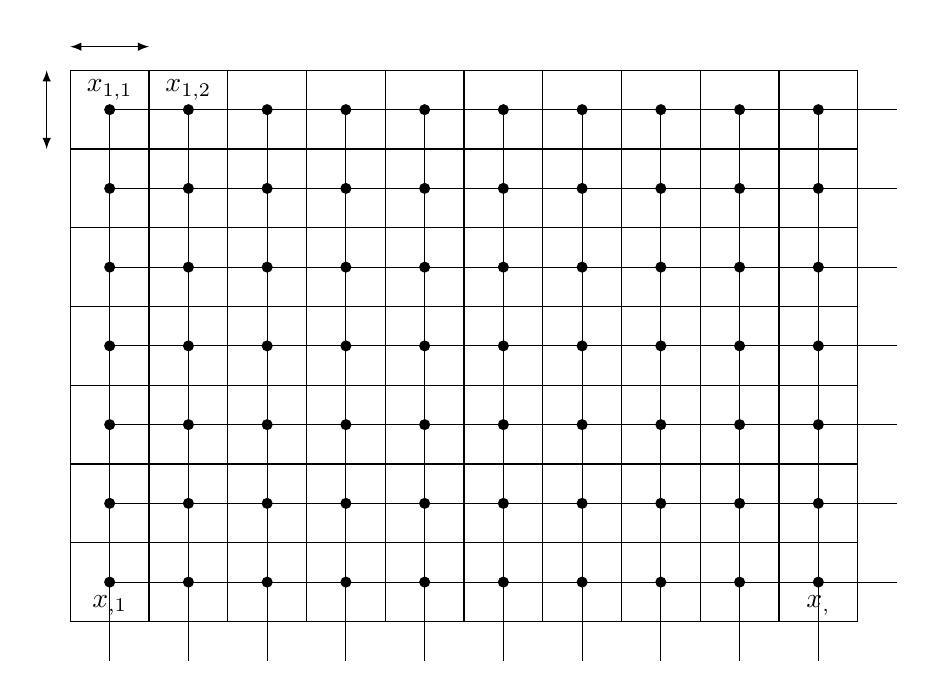
\begin{tikzpicture}
		\foreach \ii in {0,1,...,7} {
			\draw (0, \ii) -- ++(10, 0);
		}
		\foreach \jj in {0,1,...,10} {
			\draw (\jj, 0) -- ++(0, 7);
		}
		\begin{scope}[xshift=.5cm, yshift=.5cm]
		\foreach \ii in {0,1,...,6} {
			\foreach \jj in {0,1,...,9} {
				\ifthenelse{\jj<9}{\draw (\jj, \ii) -- ++(1, 0);}{}
				\ifthenelse{\ii>0}{\draw (\jj, \ii) -- ++(0, -1);}{}
				\fill (\jj,\ii) circle (0.2em);
			}
		}
		\end{scope}
		\draw[latex-latex] (0, 7.3) -- ++(1, 0) node [midway, above] {\( \PixelSize \)};
		\draw[latex-latex] (-.3, 7) -- ++(0, -1) node [midway, left] {\( \PixelSize \)};
		\node at (0.5, 6.75) {\( x_{\num{1},\num{1}} \)};
		\node at (1.5, 6.75) {\( x_{\num{1},\num{2}} \)};
		\node at (0.5, .2) {\( x_{\Height,\num{1}} \)};
		\node at (9.5, .2) {\( x_{\Height,\Width} \)};
	\end{tikzpicture}
	\caption[Representation of an image]{%
		Images are represented as a regular grid of square pixels with length \( d \).
		We represent an image as a matrix \( x \in \R^{\Height\times\Width} \).
	}%
	\label{fig:image representation}
\end{figure}
\subsection{Quality metrics}
As much of this thesis is concerned with recovering images from incomplete data, we need quantitative methods to measure the success of an algorithm.
The most widespread quality metric\footnote{%
	The name quality metric might imply that \enquote{larger is better}.
	This is not necessarily the case in this thesis.
} in signal processing is the \gls{mse}:
\begin{definition}[Mean squared error]%
	\label{def:mse}
	Let \( x, \hat{x} \in \R^{\Height\times\Width} \) be two images.
	The \emph{\glsxtrlong{mse}} between \( x \) and \( \hat{x} \) is
	\begin{equation}
		\frac{\num{1}}{\Height\Width} \sum_{i,j=\num{1}}^{\Height,\Width} (x_{i,j} - \hat{x}_{i,j})^{\num{2}} = \frac{\num{1}}{\Height\Width}\norm{x - \hat{x}}_{\num{2}}^{\num{2}}.
	\end{equation}
\end{definition}
To account for the scale of the image\footnote{%
	For instance, \( F = \interval{\num{0}}{\num{1}} \) versus \( F = \interval{\num{0}}{\num{255}} \)%
}, the \gls{mse} can be normalized by the \enquote{power} of the reference signal, leading to the definition of the \gls{nmse}.
\begin{definition}[Normalized mean squared error]
	\label{def:nmse}
	Let \( x \in \R^{\Height\times\Width} \) be a reference signal that we aim to recover and let \( \hat{x} \in \R^{\Height\times\Width} \) be an estimation.
	The \emph{\glsxtrlong{nmse}} between \( x \) and \( \hat{x} \) is
	\begin{equation}
		\frac{\norm{x - \hat{x}}_{\num{2}}^{\num{2}}}{\norm{x}_{\num{2}}^{\num{2}}}.
	\end{equation}
\end{definition}
While the \gls{mse} is symmetric in the arguments, the \gls{nmse} is not.
In the latter, the \gls{mse} is normalized by dividing by the power of the \emph{reference signal}, as otherwise we could make the error arbitrarily small by increasing the norm of the estimation (for instance via multiplication by a scalar).

Another related metric is the \gls{psnr} which is usually shown logarithmically (in decibel (\unit{\decibel})).
It represents the ratio between the highest possible power in the signal and the \gls{mse}.
\begin{definition}[Peak signal to noise ratio]%
	\label{def:psnr}
	Let \( x, \hat{x} \in \R^{\Height\times\Width} \) be two images and \( \MaxIntensity \in \R \) be the highest possible pixel intensity.
	The \emph{\glsxtrlong{psnr}} between \( x \) and \( \hat{x} \) is
	\begin{equation}
		\num{10}\log_{\num{10}} \biggl( \frac{\Height\Width \MaxIntensity^{\num{2}}}{\norm{x - \hat{x}}_{\num{2}}^{\num{2}}} \biggr).
\end{equation}
\end{definition}
The highest possible pixel intensity may or may not be well defined.
For instance, in \gls{mri} reconstruction with the fastMRI~\cite{zbontar_fastmri_2018} knee dataset, it depends on scanner-specific details and ranges over multiple orders of magnitude.
Thus, in~\cref{chap:deep neural regularizers}, we define the highest possible pixel intensity \emph{per image} as \( \max_{i,j} x_{i,j} \).
For natural images in~\cref{chap:pogmdm}, we use \(\MaxIntensity = 1 \) for all images, irrespective of whether this value is achieved in a particular image or not.

\Gls{mse}, \gls{nmse}, and \gls{psnr} all measure individual pixel differences and without any invariance properties.\footnote{%
	For example, invariance to scalar multiplication, since \enquote{brightness} can be adjusted in image viewers.
}
These metrics do not align well with the human visual system.
To demonstrate, we construct five corrupted images \( \hat{x}_{\num{1}},\hat{x}_{\num{2}},\dotsc,\hat{x}_{\num{5}} \in \R^{\numproduct{256x256}} \) with the same \gls{mse} to the reference image \( x \in \interval{\num{0}}{\num{1}}^{\numproduct{256x256}} \),\footnote{%
	Since the reference image is the same, they consequently also have the same \gls{nmse}.
} i.e.\ they are on the hypersphere \( \Set{y \in \R^{\numproduct{256x256}} \given \norm{x - y}_{\num{2}}^{\num{2}}/\num{256}^{\num{2}} = r} \) with \( r = \num{2.2e-3} \).
These corruptions are
\begin{enumerate}
	\item Adding a constant offset:
		\( \hat{x}_{\num{1}} = x + o \) for some \( o > \num{0} \).
		We used \( o = \num{0.047} \).
	\item Contrast enhancement:
		\( \hat{x}_{\num{2}} = c(x - \mu) + \mu \) for some \( c > \num{0} \), where \( \mu = \sum_{i,j=1}^{\Height,\Width} x_{i,j} \).
		We used \( c = \num{1.287} \).
	\item Salt and pepper noise: \( (\hat{x}_{\num{3}})_{i, j} = \begin{cases}
			\num{1} & \text{if}\ (i, j) \in \mathcal{S}, \\
			\num{0} & \text{if}\ (i, j) \in \mathcal{P} \setminus \mathcal{S}, \\
			x_{i, j} & \text{if}\ (i, j) \notin \mathcal{S} \cup \mathcal{P}, \\
		\end{cases} \) where \( \mathcal{S} \) and \( \mathcal{P} \) are sets of indices\footnote{All possible indices are in \( \mathcal{S} \) or \( \mathcal{P} \) with a chance of \num{3.8e-3}}.
	\item Blur: \( \hat{x}_4 = \Convolved{b}{x} \) where \( b \) is a \numproduct{4x4} uniform filter.
	\item JPEG compression: \( \hat{x}_{\num{5}} \) is a JPEG compression of \( x \).\footnote{We used imagemagick's \texttt{convert reference.png -quality 6 jpeg.jpg}}
\end{enumerate}

The results in~\cref{fig:mse doesnt correspond to human visual assessment} reveal that, despite having the same \gls{mse}, these images appear vastly different to a human observer.
Adding a constant offset has minimal perceptual impact, whereas severe JPEG compression impairs visual quality significantly.
\begin{figure*}
	\begin{tikzpicture}
		\def\mywidth{4cm}
		\def\myrad{6cm}
		\def\ssims{{0.99,0.92,0.83,0.75,0.67}}
		\node (ref) at (0, 0) {\includegraphics[width=\mywidth]{metrics/reference}};
		\draw (ref) to [out=-10, in=30] ++(2.5, -1) node [below] {\( x \)};
		\draw [ultra thick] (0, 0) circle (\myrad);
		\draw (2, -5.8) to [out=-80, in=140] ++(.5, -1.5) node [right] {\( \Set{y \in \R^{\numproduct{256x256}} \given \norm{x - y}_{\num{2}}^{\num{2}} = r^\prime} \)};
		\foreach [count=\iname] \nname in {mean, contrast, impulse, blur, jpeg}{%
			% + 36 just to offset it
			\pgfmathsetlengthmacro{\xx}{cos(\iname * 360 / 5 + 36) * \myrad}
			\pgfmathsetlengthmacro{\yy}{sin(\iname * 360 / 5 + 26) * \myrad}
			\node at (\xx, \yy) {\includegraphics[width=\mywidth]{metrics/\nname}};
			\pgfmathsetlengthmacro{\yyanno}{\yy + \mywidth/2+.3cm}
			\node at (\xx, \yyanno) {\( \hat{x}_{\iname} \)};
			\pgfmathsetlengthmacro{\xxssim}{\xx - 1.9cm}
			\pgfmathsetlengthmacro{\yyssim}{\yy + 1.6cm}
			\pgfmathsetmacro{\ssim}{\ssims[\iname-1]}
			\node [right, rounded corners, fill=white] at (\xxssim, \yyssim) {\ifthenelse{\iname=1}{SSIM=}{}\num{\ssim}};
		}
	\end{tikzpicture}
	\caption[Images on the MSE hypersphere appear vastly different to the human]{%
		The corrupted images \( \hat{x}_{\num{1}},\dotsc,\hat{x}_{\num{5}} \) all have the same \gls{mse} with respect to the reference image \( x \).
		However, to a human they appear vastly different.
		The image \( x_{\num{1}} \), where the same constant offset is added to each pixel, is \enquote{the same} as the original image \( x \) to the human observer.
		On the other hand, the image \( x_{\num{5}} \), which has undergone severe JPEG compression, has lost many details and looks much worse to the human.
		The inlays show the \glsxtrshort{ssim} value (the images are ordered in decreasing \glsxtrshort{ssim} counterclockwise from twelve o'clock), which align much closer with human assessment.
	}%
	\label{fig:mse doesnt correspond to human visual assessment}
\end{figure*}
This discrepancy poses a problem if the output of an algorithm is presented to a human, for instance, for diagnosis or entertainment.

Numerous quality metrics have been proposed to address this issue and we refer to~\cite{mason_imagequality_2020} for a small overview and a study of how well quality metrics predict radiologists' performance.
In this thesis, we use the popular \gls{ssim}.
The definition of the \gls{ssim} is understood locally on small patches; the image-level metric is the mean over all overlapping patches, with a filter to avoid blocking artifacts.
\begin{definition}[Structural similarity]%
	\label{def:ssim}
	Let \( x, \hat{x} \in \R^{d \times d} \) be two image patches and let \( \mu_{x}, \mu_{\hat{x}} \in \R \) and \( \sigma_x, \sigma_{\hat{x}} > \num{0} \) be their mean and standard deviation respectively, e.g.\ \( \mu_{x} = \tfrac{1}{d^{\num{2}}} \sum_{i,j=\num{1}}^{d,d} x_{i,j} \) and \( \sigma_x^{\num{2}} = \frac{1}{d^{\num{2}}-\num{1}} \sum_{i,j=\num{1}}^{d,d} (x_{i,j} - \mu_x)^{\num{2}} \).
	In addition, let \( \operatorname{cov}_{x\hat{x}} = \frac{1}{d^{\num{2}}-1} \sum_{i,j=\num{1}}^{d,d} (x_{i,j}- \mu_x)(\hat{x}_{i,j} - \mu_{\hat{x}}) \) and let \( K_{\num{1}} > \num{0} \) and \( K_{\num{2}} > \num{0} \).
	The \emph{\glsxtrlong{ssim}} between \( x \) and \( \hat{x} \) is
	\begin{equation}
		\frac{(\num{2}\mu_x\mu_{\hat{x}} + C_{\num{1}})(\num{2}\operatorname{cov}_{x\hat{x}} + C_{\num{2}})}{(\mu_x^{\num{2}}+\mu_{\hat{x}}^{\num{2}} + C_{\num{1}})(\sigma_x^{\num{2}} + \sigma_{\hat{x}}^{\num{2}} + C_{\num{2}})}
	\end{equation}
	where \( C_{\num{1}} = (K_{\num{1}}m)^{\num{2}} \) and \( C_{\num{2}} = (K_{\num{2}}m)^{\num{2}} \) with \( \MaxIntensity \in \R \) defined as in~\cref{def:psnr}.
\end{definition}

\Gls{ssim} can be decomposed into components comparing \enquote{luminance}, \enquote{contrast}, and \enquote{structure}, for details see the original publication~\cite{wang_ssim_2004}.
In this thesis, we use a \numproduct{7x7} uniform filter\footnote{%
	This means that, in the above definition, \( d = \num{7} \) and the image patches are essentially taken directly (without filtering).%
} and standard choices \( K_{\num{1}} = \num{0.01} \) and \( K_{\num{2}} = \num{0.03} \).
As for the \gls{psnr}, when the highest pixel intensity is not well defined, we take the highest pixel intensity in the reference image.
\Cref{fig:mse doesnt correspond to human visual assessment} shows \gls{ssim} as inlays; with images ordered in decreasing \gls{ssim} (counterclockwise from twelve o'clock), demonstrating that \gls{ssim} provides a better alignment with human assessment.
